\documentclass[nostrict]{szablonPG}


\usepackage{pdfpages}
\usepackage{multicol} % do sk³adu w dwóch kolumnach
\usepackage[nottoc]{tocbibind}
\usepackage[unicode=true]{hyperref}
\usepackage{graphicx}
\usepackage{float}
\usepackage{siunitx}
\usepackage{caption}
\raggedbottom
\usepackage[singlelinecheck=false % <-- important
]{caption}
\newcommand{\desctotoc}[1]{%
	\addtocontents{toc}{\medskip\noindent\detokenize{#1}\leavevmode\par\medskip}
}
\setcounter{secnumdepth}{4}
\begin{document}
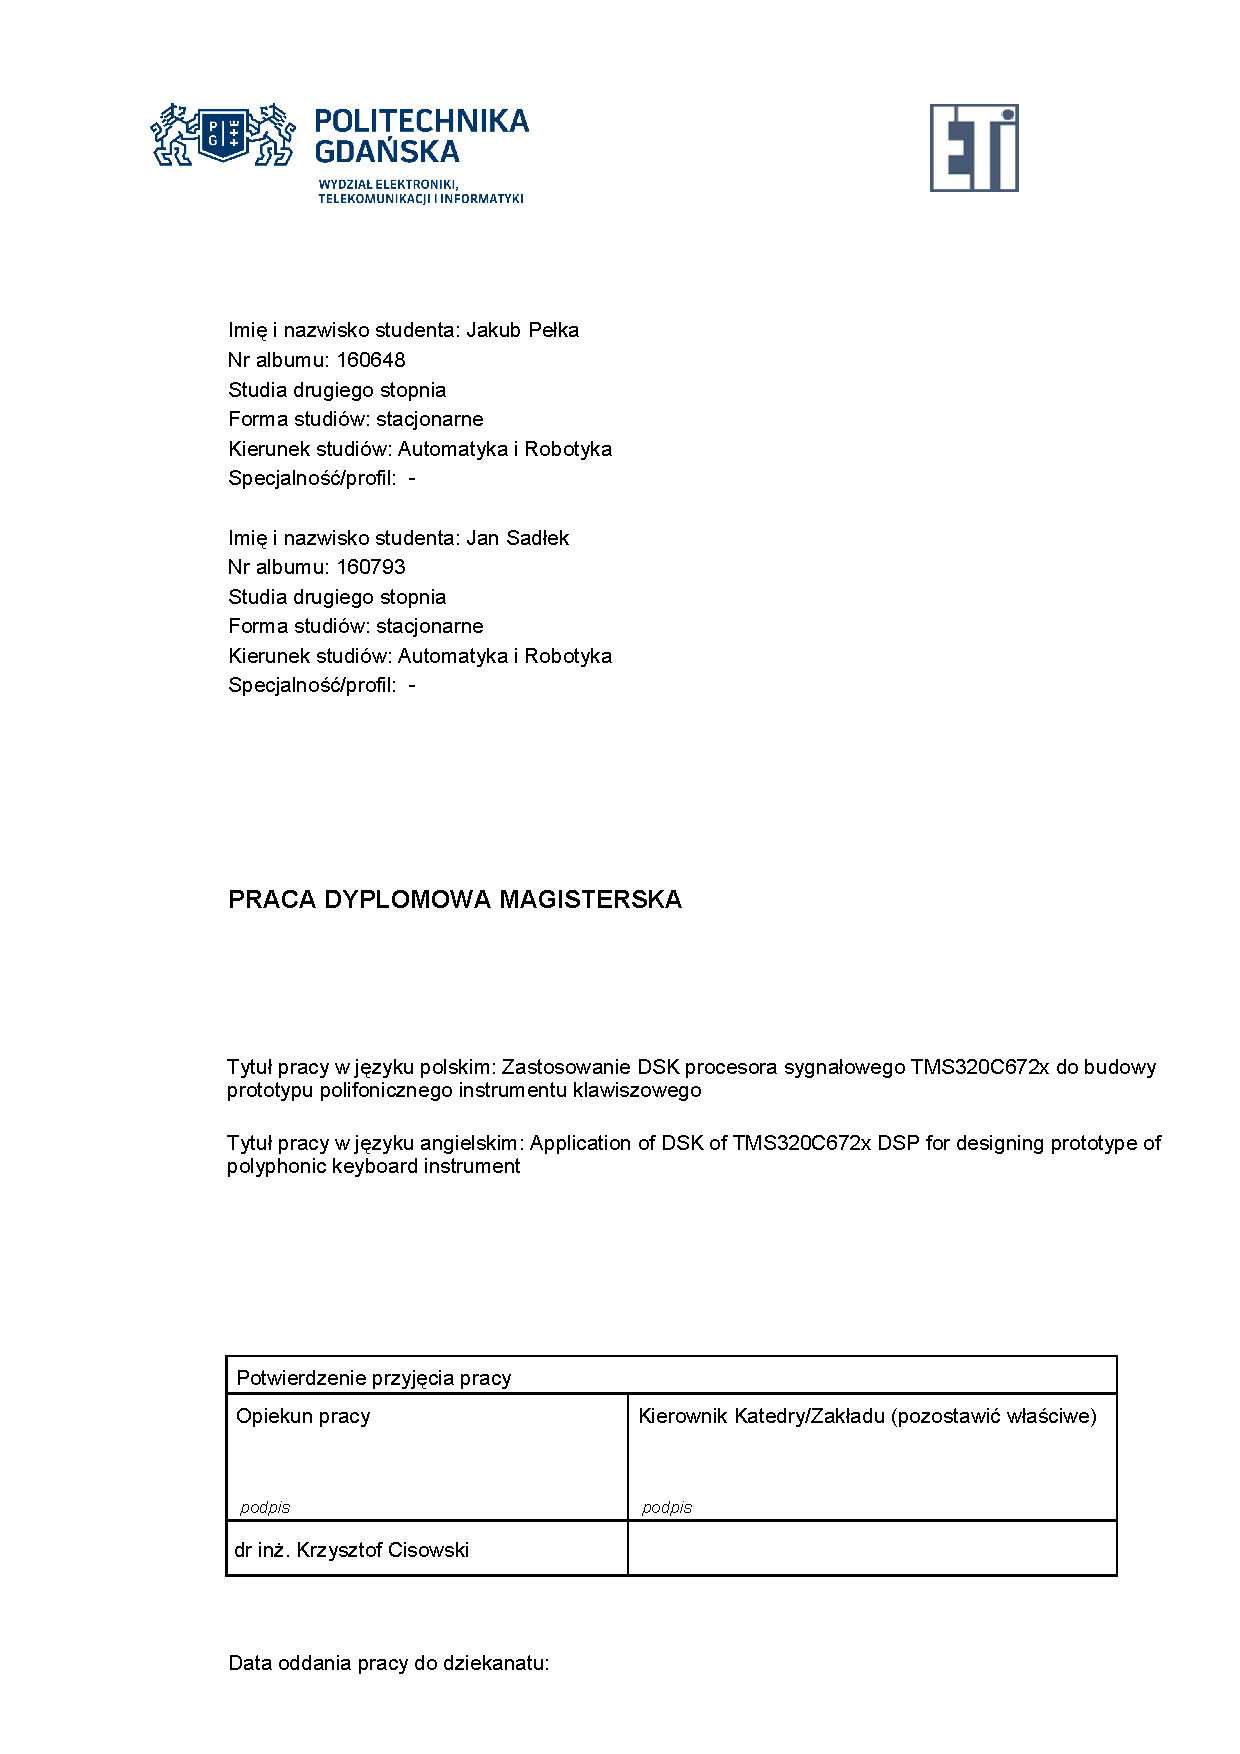
\includepdf[pages=-]{StronaTytulowa_160648.pdf}
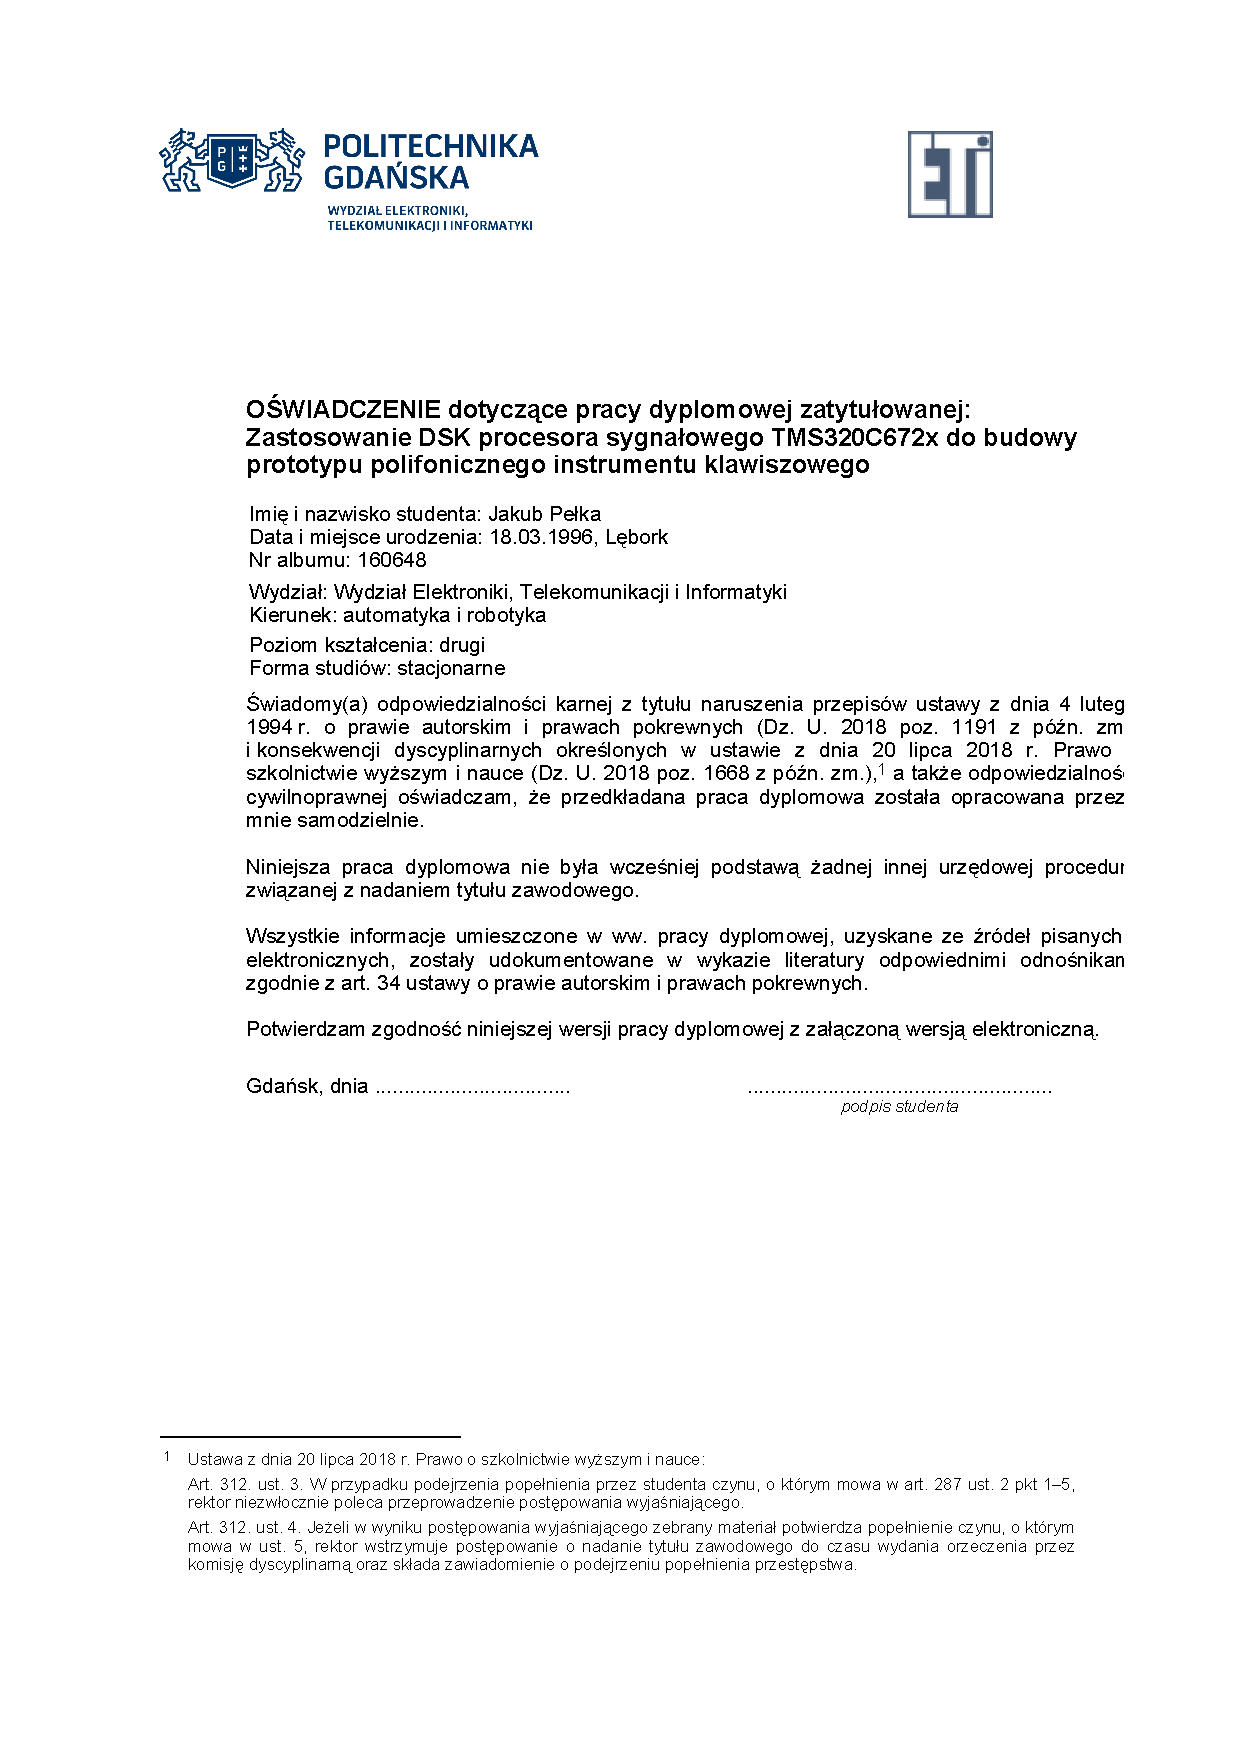
\includepdf[pages=-]{Oswiadczenie_160648.pdf}

	\setcounter{page}{3}
	\let\cleardoublepage\clearpage
	\chapter*{Streszczenie}
W ramach pracy wykonano prototyp syntezatora muzycznego. Platformę sprzętową stanowi płyta Professional Audio Development Kit (PADK) firmy Lyrtech wyposażona w procesor sygnałowy TMS320C6727 firmy Texas Instruments. Sterowanie pracą instrumentu zostało zrealizowane za pomocą klawiatury MIDI. Opisano i zaimplementowano następujące metody syntezy dźwięku: subtraktywną, addytywną, modulację FM oraz modelowania fizycznego. Utworzono graficzny interfejs użytkownika działający na komputerze klasy PC, który umożliwia zmianę parametrów generowanego dźwięku.
\newline
\\
\textbf{Słowa kluczowe}: instrument muzyczny, syntezator, synteza dźwięku, addytywna, subtraktywna, modelowanie fizyczne, cyfrowy falowód, modulacja częstotliwości, klawiatura midi, polifonia.
\\
\\
\textbf{Dziedzina nauki i techniki, zgodnie z wymogami OECD:} Nauki inżynieryjne i techniczne, elektrotechnika, elektronika, inżynieria informatyczna, sprzęt komputerowy i architektura komputerów.
	\chapter*{Abstract}
Within this thesis a prototype of a musical synthesizer was made. The hardware consisted of a Lyrtech Professional Audio Development Kit (PADK) which was equipped with a Texas Instruments digital signal processor TMS320C6727. The instrument's operation was controlled using a MIDI keyboard. The following methods of sound synthesis were described and implemented: subtractive, additive, frequency modulation and physical modeling. A graphical user interface, which allows to set up the parameters of generated sound, was created on a personal computer.
\newline
\\
\textbf{Keywords}: musical instrument, synthesizer, sound synthesis, additive, subtractive, physical modeling, digital waveguide, frequency modulation, MIDI keyboard, polyphony.


%	\tableofcontents    % spis treœci
	
	\chapter*{SPIS TREŚCI} 
\contentsline {chapter}{Wykaz wa\IeC {\.z}niejszych oznacze\IeC {\'n} i skr\IeC {\'o}t\IeC {\'o}w}{6}{chapter*.3}
\contentsline {chapter}{\numberline {1}Wst\IeC {\k e}p i cel pracy (Autor: Jan Sadłek)}{7}{chapter.1}
\contentsline {chapter}{\numberline {2}Wprowadzenie (Autor: Jan Sadłek)}{8}{chapter.2}
\contentsline {section}{\numberline {2.1}Dźwięk}{8}{section.2.1}
\contentsline {section}{\numberline {2.2}Linearyzacja i model w przestrzeni stanu }{10}{section.2.2}
\contentsline {subsection}{\numberline {2.2.1}\IeC {\'S}rodek masy i o\IeC {\'s} obrotu w tym samym punkcie}{10}{subsection.2.2.1}
\contentsline {subsection}{\numberline {2.2.2}\IeC {\'S}rodek masy i o\IeC {\'s} obrotu w r\IeC {\'o}\IeC {\.z}nych punktach}{11}{subsection.2.2.2}
\contentsline {section}{\numberline {2.3}Transmitancja obiektu }{12}{section.2.3}
\contentsline {chapter}{\numberline {3}Obiekt regulacji (Autor: Jakub Pełka)}{13}{chapter.3}
\contentsline {section}{\numberline {3.1}Wahad\IeC {\l }o firmy Bytronic}{13}{section.3.1}
\contentsline {section}{\numberline {3.2}Sprz\IeC {\k e}towe rozwi\IeC {\k a}zanie pomiarowo-steruj\IeC {\k a}ce}{14}{section.3.2}
\contentsline {section}{\numberline {3.3}Pomiary w\IeC {\l }a\IeC {\'s}ciwo\IeC {\'s}ci uk\IeC {\l }adu}{18}{section.3.3}
\contentsline {subsection}{\numberline {3.3.1}Przetwornik cyfrowo-analogowy}{18}{subsection.3.3.1}
\contentsline {subsection}{\numberline {3.3.2}Charakterystyka sygna\IeC {\l }u steruj\IeC {\k a}cego}{19}{subsection.3.3.2}
\contentsline {subsection}{\numberline {3.3.3}Napi\IeC {\k e}cie zasilaj\IeC {\k a}ce silnik}{20}{subsection.3.3.3}
\contentsline {subsection}{\numberline {3.3.4}Si\IeC {\l }a dzia\IeC {\l }aj\IeC {\k a}ca na w\IeC {\'o}zek}{20}{subsection.3.3.4}
\contentsline {subsection}{\numberline {3.3.5}Charakterystyki czujnik\IeC {\'o}w}{22}{subsection.3.3.5}
\contentsline {chapter}{\numberline {4}Badanie w\IeC {\l }a\IeC {\'s}ciwo\IeC {\'s}ci uk\IeC {\l }adu}{24}{chapter.4}
\contentsline {section}{\numberline {4.1}Przewidywana transmitancja (Autor: Bartosz Filipów)}{24}{section.4.1}
\contentsline {section}{\numberline {4.2}Badanie w\IeC {\l }a\IeC {\'s}ciwo\IeC {\'s}ci obiektu (Autor: Jakub Pełka)}{25}{section.4.2}
\contentsline {section}{\numberline {4.3}Analiza uzyskanej transmitancji (Autor: Bartosz Filipów)}{27}{section.4.3}
\contentsline {section}{\numberline {4.4}Por\IeC {\'o}wnanie modelu teoretycznego i zbadanego (Autor: Bartosz Filipów)}{28}{section.4.4}
\contentsline {chapter}{\numberline {5}Regulacja w przestrzeni stanu }{29}{chapter.5}
\contentsline {section}{\numberline {5.1}Sterowalno\IeC {\'s}\IeC {\'c} (Autor: Bartosz Filipów)}{29}{section.5.1}
\contentsline {section}{\numberline {5.2}Obserwowalno\IeC {\'s}\IeC {\'c} (Autor: Bartosz Filipów)}{29}{section.5.2}
\contentsline {section}{\numberline {5.3}Obserwator stanu (Autor: Jakub Pełka)}{31}{section.5.3}
\contentsline {section}{\numberline {5.4}Stabilno\IeC {\'s}\IeC {\'c} (Autor: Bartosz Filipów)}{33}{section.5.4}
\contentsline {section}{\numberline {5.5}Regulator (Autor: Bartosz Filipów)}{34}{section.5.5}
\contentsline {chapter}{\numberline {6}Badanie uk\IeC {\l }adu sterowania}{36}{chapter.6}
\contentsline {section}{\numberline {6.1}Macierz wag stan\IeC {\'o}w (Autor: Bartosz Filipów)}{36}{section.6.1}
\contentsline {subsection}{\numberline {6.1.1}Wp\IeC {\l }yw wagi stanu po\IeC {\l }o\IeC {\.z}enia w\IeC {\'o}zka}{37}{subsection.6.1.1}
\contentsline {subsection}{\numberline {6.1.2}Wp\IeC {\l }yw wagi stanu wychylenia wahad\IeC {\l }a}{37}{subsection.6.1.2}
\contentsline {subsection}{\numberline {6.1.3}Wp\IeC {\l }yw wagi stanu pr\IeC {\k e}dko\IeC {\'s}ci w\IeC {\'o}zka i wagi stanu pr\IeC {\k e}dko\IeC {\'s}ci k\IeC {\k a}towej wahad\IeC {\l }a}{38}{subsection.6.1.3}
\contentsline {section}{\numberline {6.2}Wp\IeC {\l }yw modelu matematycznego obiektu na jako\IeC {\'s}\IeC {\'c} sterowania (Autor: Bartosz Filipów)}{39}{section.6.2}
\contentsline {section}{\numberline {6.3}Ko\IeC {\'n}cowe strojenie uk\IeC {\l }adu (Autor: Jakub Pełka)}{40}{section.6.3}
\contentsline {chapter}{\numberline {7}Podsumowanie (Autor: Bartosz Filipów)}{42}{chapter.7}
\contentsline {chapter}{Spis rysunk\'ow}{43}{chapter*.44}
\contentsline {chapter}{Spis tabel}{45}{chapter*.45}
\contentsline {chapter}{Bibliografia}{46}{chapter*.46}
\contentsline {chapter}{\numberline {8}Dodatek A -- Schemat elektryczny uk\IeC {\l }adu}{47}{chapter.8}
\contentsfinish 

	\addcontentsline{toc}{chapter}{Wykaz ważniejszych oznaczeń i skrótów}
\chapter*{Wykaz ważniejszych oznaczeń i skrótów}

\begin{tabular}{lcl}
	\textit{SH} & -- & składowe harmoniczne. \\
	\textit{DSP} & -- & ang. digital signal processor -- procesor sygnałowy \\
	\textit{FM} & -- & ang. frequency modulation -- modulacja częstotliwości \\
	\textit{AM} & -- & ang. amplitude modulation -- modulacja amplitudy \\
	\textit{CS} & -- & cyfrowy syntezator \\
	\textit{AS} & -- & analogowy syntezator \\
	\textit{MIDI} & -- & ang. Musical Instrument Digital Interface -- cyfrowy interfejs instrumentów muzycznych \\
	\textit{DFT} & -- & ang. Discrete Fourier Transform -- Dyskretna transformata Fouriera \\
	\textit{VCO} & -- & ang. voltage-controlled oscillator -- oscylator kontrolowany napięciem \\
	\textit{VCA} & -- & ang. voltage-controlled amplifier -- wzmacniacz kontrolowany napięciem \\
	\textit{VCF} & -- & ang. voltage-controlled filter -- filtr kontrolowany napięciem \\
	\textit{LFO} & -- & ang. low-frequency oscillation -- generator wolnych przebiegów \\
	\textit{ADSR} & -- & ang. attack, delay, sustain, release -- generator obwiedni \\
	\textit{DAC} & -- & ang. digital-to-analog converter -- przetwornik cyfrowo-analogowy \\
	\textit{CPU} & -- & ang. central processing unit -- procesor \\
	\textit{FPGA} & -- & ang. field-programmable gate array -- bezpośrednio programowalna macierz bramek \\
	\textit{JTAG} & -- & ang. Joint Test Action Group -- protokół testowania połączeń \\
	\textit{ISR} & -- & ang. interrupt service handler -- obsługa przerwania \\
	\textit{FIR} & -- & ang. finite impulse response -- skończona odpowiedź impulsowa \\
	\textit{STS} & -- & ang. short term spectrum -- krótkie okno widmowe \\
	\textit{IIR} & -- & ang. infinite impulse response -- nieskończona odpowiedź impulsowa \\
\end{tabular} 

	\chapter{Wstęp i cel pracy}
Muzyka jest ważnym aspektem życia każdego człowieka. Jest to dziedzina, która była rozwijana już od czasów prehistorycznych. %Napisac o instrumentach klasycznych. Instrumenty używały drgające struny, membrany , idiofony (marimba), Podac przyklady
%https://mlodytechnik.pl/eksperymenty-i-zadania-szkolne/wynalazczosc/29983-historia-wynalazkow-instrumenty-muzyczne
Na początku ludzie wykorzystywali proste instrumenty rytmiczne takie jak bębny czy grzechotki, które służyły do rytuałów plemiennych. W starożytności wynaleziono instrumenty dęte oraz strunowe. W okresie średniowiecza i renesansu powstały instrumenty smyczkowe, chordofony (na przykład klawesyn) oraz aerofony (na przykład organy).
Wraz z rozwojem technologicznym, ludzie zaczęli używać skomplikowanych urządzeń do tworzenia muzyki. W pierwszej połowie XX wieku zaczęto używać instrumentów bazujących na układach scalonych.
% ogarnac po krótce budowe analogowych jak sie rozwijała
Na początku potrafiły one wydobywać z siebie proste dźwięki. Z czasem zaczęły posiadać coraz większe możliwości brzmieniowe. W drugiej połowie XX wieku cyfrowe instrumenty klawiszowe zaczęły być dostępne dla szerokiego kręgu odbiorców. Technologia cyfrowego przetwarzania sygnałów stworzyła nowe możliwości dla kompozytorów muzyki elektronicznej.

Syntezatory analogowe posiadały wiele niedoskonałości: nie pozwalały na precyzyjne odtworzenie pożądanych charakterystyk filtrów, miały ograniczone możliwości modelowania dźwięku oraz często z powodu starzenia się elementów elektronicznych zmieniały swoje parametry z upływem czasu. Dziedzina nauki zajmująca się syntezą dźwięku zaczęła dynamicznie rozwijać się wraz z rozwojem procesorów sygnałowych (DSP). Pojawienie się technologii cyfrowego przetwarzania sygnałów umożliwiło tworzenie dużo bardziej skomplikowanych brzmień. Procesory sygnałowe pozwalały na praktycznie nieograniczone zmiany charakterystyk generowanych dźwięków. Jednak zmiana sposobu syntezy z analogowej na cyfrową spowodowała pojawienie się również nowe ograniczenia. W systemach cyfrowych pojawił się problem doboru próbkowania sygnałów wejściowych wpływający na szerokość pasma ich przetwarzania.
Ważnym ograniczeniem była konieczność optymalizacji czasu wykonywania skomplikowanych algorytmów, wynikająca z konieczności ich zakończenia, do momentu pobrania kolejnej próbki.

Motywem realizacji tej pracy jest możliwość badania różnych metod syntezy dźwięku na procesorze sygnałowym. 
Autorzy zwrócili uwagę, iż w dotychczas spotykanych syntezatorach, próby imitacji brzmień naturalnych instrumentów, są dalekie od doskonałości.

Celem tej pracy było zrealizowanie polifonicznego instrumentu klawiszowego, który będzie wykorzystywał kilka typowych metod syntezy dźwięku. Realizacja projektu opierała na zestawie uruchomieniowym Professional Audio Development firmy Lyrtech procesora sygnałowego TMS320C6727 oraz klawiaturze z interfejsem USB MIDI. Jednym z celów było również wykorzystanie dużych możliwości obliczeniowych zastosowanego procesora. Głównymi zadaniami do wykonania były:

\begin{enumerate}
    \item opracowanie i implementacja na procesorze sygnałowym algorytmów generowania 	wielotonów harmonicznych i dźwięków szumowych,
    
    \item opracowanie metod sterowania barwą generowanych dźwięków dla różnych metod syntezy barw,
    
    \item realizacja interfejsu użytkownika.
\end{enumerate}
W niniejszej pracy omówiono realizację powyższych celów.

W rozdziale drugim przedstawiono informacje teoretyczne z zakresu teorii muzyki, podstaw syntezy dźwięku oraz cyfrowego przetwarzania sygnałów. W celu uzasadnienia wyboru cyfrowej syntezy dźwięku, przedstawiono porównanie wad i zalet metod analogowych i cyfrowych przetwarzania sygnałów. Informację tam zamieszczone są niezbędne do pełnego zrozumienia dalszej części pracy.

W rozdziale trzecim zaprezentowano implementację autorskiego instrumentu klawiszowego – sprzętową oraz programową. Opis działania programu oraz własności platformy sprzętowej pozwala na swobodną prezentację w dalszych rozdziałach pracy implementacji metod syntezy dźwięku. Zaprezentowano poszczególne moduły programu, w tym algorytm FFT na procesorze oraz metody sterowania protokołu MIDI. W tym samym rozdziale autorzy opisali realizację interfejsu instrumentu klawiszowego. Umożliwia on wybieranie odpowiedniej metody tworzenia dźwięku oraz dobranie parametrów ich syntezy. Interfejs zaimplementowano jako aplikację okienkową na komputerze PC, komunikującą się z programem działającym na procesorze sygnałowym.

W kolejnych czterech rozdziałach opisano metody syntezy dźwięków, które wykorzystywane są w instrumentach klawiszowych. Każdy z nich przedstawia teorię z zakresu danej metody, a następnie jej realizację praktyczną. Rozdział czwarty przedstawia najczęściej wykorzystywaną metodę syntezy – algorytm subtraktywny, który jest powszechnie wykorzystywany w syntezatorach analogowych. W rozdziale piątym zaprezentowano metodę addytywną oraz sposób generowania za jej pomocą dźwięku organów. W rozdziale szóstym omówiono syntezę dźwięku z użyciem modulacji częstotliwości (metoda FM). W rozdziale siódmym przedstawiono najbardziej skomplikowaną metodę syntezy omówioną w tej pracy – metodę modelowania matematycznego. Metoda ta wykorzystywana jest obecnie głównie w laboratoriach naukowych, gdyż daje największe możliwości uzyskania pożądanych brzmień syntezowanych dźwięków.

Rozdział ósmy jest podsumowaniem całej pracy. Omówiono w nim sposób realizacji przyjętych celów oraz przedstawiono wnioski końcowe.
	\chapter{Wprowadzenie teoretyczne}\label{chapter2}

W niniejszym rozdziale omówiono podstawowe pojęcia związane z dziedziną muzyki, syntezy dźwięku oraz przetwarzania sygnałów cyfrowych. Omówione zagadnienia odnoszą się do całości pracy, nie są one powiązane z poszczególnymi metodami syntezy. Przedstawienie ich w początkowej części pracy, ma na celu ułatwienie czytelnikowi zrozumienia kolejnych rozdziałów.



\section{Dźwięk}
Dźwięk można rozpatrywać w dwóch aspektach: fizycznym oraz muzycznym. Z fizycznego punktu widzenia, dźwięk jest zaburzeniem falowym w ośrodku sprężystym gazowym, ciekłym lub stałym, który wywołuje wrażenie słuchowe u człowieka \cite{dzwiek_pwn}. Poddziedzina fizyki, zajmująca się ściśle tematem dźwięku, nazywana jest akustyką.

W muzyce, dźwięk rozpatrywany jest jako zjawisko, które wydobywane jest z instrumentów muzycznych lub generowane za pomocą głosu ludzkiego. Główne właściwości dźwięku w muzyce, to:

\begin{itemize}
	\item wysokość dźwięku - jest zależna od wartości częstotliwości podstawowej dźwięku (pierwszej harmonicznej),
	
	\item czas trwania - zależny od czasu emisji dźwięku na danym instrumencie,
	
	\item głośność - zależna od amplitudy drgań powietrza przenoszącego dźwięk,
	
	\item barwa dźwięku - zależna od liczby i częstotliwości poszczególnych składowych harmonicznych (SH) dźwięku oraz zmian ich amplitudy w czasie. Jako SH rozumiane są składowe sinusoidalne dźwięku, które są całkowitymi wielkrotnościami częstotliwości podstawowej danego dźwięku \cite{synth_brief_intro}.
	% (źródło: https://pl.wikipedia.org/wiki/D%C5%BAwi%C4%99k_(muzyka))
\end{itemize}

W celu ustandardyzowania dźwięków w utworach muzycznych wprowadzono skale dźwiękowe. Obecnie w muzyce europejskiej stosowana jest skala dwunastotonowa równomiernie temperowana. Odległości między tymi dźwiękami nazywane są interwałami, które wyraża się w jednostkach półtonów. Istnieje zależność między kolejnymi półtonami. Może ona być wyrażona wzorem:
\begin{equation} \label{equ:wpr_dzwiek}
k = f(\sqrt[12]{2})^{n}
\end{equation}
\begin{tabular}{ l l l l}
	gdzie: 	&	$f$ & - &  częstotliwość tonu dźwięku, od którego liczona jest odległość n, \\
	&	$k$ & - &  szukana częstotliwość tonu, do którego liczona jest odległość n, \\
	&   $n$ &  - & odległość tonu o częstotliwości f od tonu o częstotliwości k w półtonach. \\
\end{tabular}

Odstęp między pierwszym a ostatnim dźwiękiem w skali nazywany jest oktawą. Mierzy on 12 półtonów. Odległość ta jest wyjątkowa, gdyż dźwięk położony o oktawę dalej od pierwszego, jest jego dwukrotnością pod względem częstotliwości podstawowej składowej harmonicznej.



\section{Rodzaje klawiatur muzycznych}
Podstawowy podział klawiatur muzycznych rozpatruje się pod względem możliwości wydobycia jednego lub kilku dźwięków przy naciśnięciu kilku klawiszy. Rodzaje te nazwano klawiaturami monofonicznymi oraz polifonicznymi.

\subsection{Klawiatura monofoniczna}
Monofonia w muzyce to faktura muzyczna utworzona z pojedynczej linii melodycznej. Aby aktualnie wykonywany fragment utworu można było nazwać monofonicznym, w poszczególnych chwilach czasu powinien być grany tylko jeden dźwięk. W odniesieniu do klawiatury cyfrowej oraz analogowej, oznacza to, iż można za ich pomocą w danej chwili czasu wytwarzać tylko jeden dźwięk. Klasycznym przykładem klawiatury monofonicznej jest syntezator analogowy Minimoog.

\subsection{Klawiatura polifoniczna}
Polifonia w muzyce oznacza występowanie kilku linii melodycznych w tym samym czasie. Polifonia klawiatury zatem oznacza możliwość wydobycia w danym momencie czasu wielu dźwięków, poprzez naciśnięcie kilku klawiszy. Pojęcie polifonicznej klawiatury muzycznej nie definiuje dokładnej liczby wydobywanych za jej pomocą dźwięków. Obecnie produkowane cyfrowe instrumenty muzyczne posiadają ograniczoną liczbę możliwych do wydobycia na raz tonów. Spowodowane jest to niewystarczającą mocą obliczeniową procesorów DSP.

%
% Voice allocation alghorithm - opisac jaki bedziemy uzywac
%

Jednym z głównych zadań niniejszego projektu magisterskiego jest implementacja polifonicznej klawiatury muzycznej.



\section{Przegląd metod syntezy dźwięku}
% http://legacy.spa.aalto.fi/publications/reports/sound_synth_report.pdf
Podział metod syntezy dźwięku w literaturze jest bardzo zróżnicowany. Najczęściej wykorzystuje się różnice w metodach syntezy \cite{metody_syntezy}:
\begin{itemize}
	\item widmowych,
	\item algorytmach abstrakcyjnych,
	\item fizycznych,
	\item przetwarzania sygnałów.
	% https://ieeexplore.ieee.org/document/4412805
\end{itemize}

W poniższych podrozdziałach scharakteryzowano poszczególne rodzaje metod syntezy dźwięku.

\subsection{Metody widmowe}
Do grupy widmowych metod syntezy dźwięku zaliczana jest synteza subtraktywna oraz addytywna. Zgodnie z nazwą, skupiają się one na syntezie brzmień w dziedzinie częstotliwości. Metoda subtraktywna zajmuje się głównie wycinaniem pasm widmowych z dźwieków o bogatym składzie harmonicznym. Metoda addytywna skupia się natomiast na dodawaniu kolejnych harmonicznych w dziedzinie częstotliwości. Obie metody zostały dokładnie omówione w rozdziałach \ref{chapter_subtractive} i~\ref{chapter_additive} niniejszej pracy.

\subsection{Algorytmy abstrakcyjne}
% https://ccrma.stanford.edu/~bilbao/booktop/node6.html
% http://legacy.spa.aalto.fi/publications/reports/sound_synth_report.pdf
Synteza za pomocą algorytmów abstrakcyjnych zazwyczaj odnosi się do zmian istniejących już dźwięków za pomocą filtrów nieliniowych lub funkcji matematycznych. Do algorytmów abstrakcyjnych należą między innymi: synteza FM, synteza AM, synteza poprzez waveshaping lub algorytm Karplus-Strong. W literaturze można również spotkać się z określaniem tej grupy metod syntezy jako Distortion synthesis (synteza poprzez zakłócanie), która odnosi się do wprowadzanych zmian w istniejącym już dźwięku (zakłóceń). W niniejszej pracy poświęcono cały rozdział metodzie syntezy FM.

\subsection{Metody fizyczne}
% https://ccrma.stanford.edu/~bilbao/booktop/node12.html
% https://edu.pjwstk.edu.pl/wyklady/mul/scb/main37.html
Metody fizyczne skupiają się na odwzorowywaniu instrumentów muzycznych poprzez tworzenie ich modeli fizycznych. Do tej grupy należy synteza dźwięku przy użyciu modelowania matematycznego, synteza komórkowa (ang. Cellular Sound Synthesis) oraz synteza falowodowa (ang. Digital Waveguide Modeling) \cite{czyzewski_dzwiek_cyfrowy}.

Metody syntezy oparte na modelach fizycznych są uważane za najbardziej naukowe i poświęcone jest im wiele prac naukowych. W niniejszej pracy, z tej grupy metod syntezy, przedstawiono głównie syntezę fizyczną opartą o falowody cyfrowe oraz modele ARMA.

\subsection{Metody przetwarzania sygnału}
%http://marcdata.hamu.cz/vyzkum/dokumenty/Lit92.pdf - additive, subtractive, FM. sampling
%https://soundlab.cs.princeton.edu/publications/survey_icmc09.pdf - 4 strona, tabelka
%https://www.youtube.com/watch?v=I64y40EIPaM
Jako metody przetwarzania sygnału rozumiane są takie metody syntezy, które oddziaływują bezpośrednio na próbki sygnału cyfrowego. Do tej grupy metod należą między innymi: synteza tablicowa (wavetable), synteza granularna oraz synteza poprzez samplowanie.

Synteza za pośrednictwem samplowania jest najbardziej powszechną syntezą dźwięku w tej grupie metod. Polega ona na użyciu fragmentu wcześniej dokonanego nagrania (sampla) i odtwarzanie go dla różnych wysokości dźwięków. Jest to obecnie metoda najczęściej używana przez kompozytorów \cite{misra_cook_przetw_syg}.

Z uwagi na nieunaukowy charakter tego rodzaju syntezy dźwięku, żadnej z tych metod nie został poświęcony żaden rozdział niniejszej pracy. Jedynie synteza wavetable została użyta jako usprawnienie syntezy addytywnej.


\section{Klasyczne moduły syntezatorów dźwięku}
%https://www.dummies.com/art-center/music/piano/common-keyboard-terms-and-abbreviations/
%https://en.wikipedia.org/wiki/Modular_synthesizer#:~:text=Modular%20synthesizers%20are%20synthesizers%20composed,user%20to%20create%20a%20patch.
Syntezatory analogowe nazywane są również modularnymi. Utworzenie dźwięku przez takie urządzenie wymaga przejścia sygnału przez kilka modułów. Źródłem sygnału jest zazwyczaj pewien oscylator lub generator szumu. Dźwięk jest tworzony w źródle, a następnie trafia do filtra. Następnie po filtracji jest wyprowadzany na wyjście układu.

\begin{figure}[H]
	\centering
	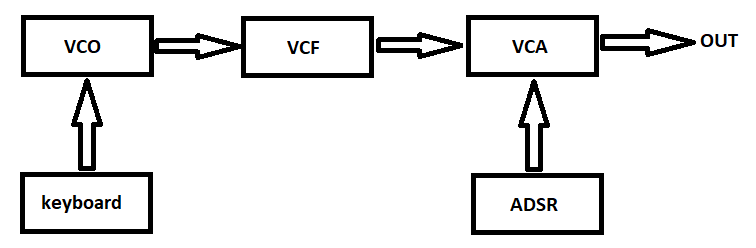
\includegraphics[width=12cm]{./grafiki/analog_synth_scheme}
	\captionsetup{justification=centering}
	\caption{Schemat podstawowego syntezatora modularnego (analogowego).}
	\label{rys:analog_scheme}
\end{figure}

Na rysunku \ref{rys:analog_scheme} przedstawiono podstawowy schemat syntezatora modularnego. Składa się on z najbardziej uniwersalnych elementów stosowanych w analogowej syntezie dźwięku. Sygnał jest tworzony przy wykorzystaniu oscylatora (VCO), którego częstotliwość zostaje ustalona poprzez naciśnięcie odpowiedniego klawisza (na klawiaturze sterującej). Następnie dźwięk, za pomocą filtra (VCF) zostaje pozbawiony pewnej części składowych harmonicznych. W dalszej kolejności dociera on do modułu sterującego amplitudą dźwięku (VCA), który ustala jego amplitudę zgodnie z ustawieniami modułu obwiedni dźwięku (ADSR). Następnie dźwięk jest wyprowadzany na wyjście (OUT), czyli do zestawu nagłośnieniowego.

W cyfrowej syntezie dźwięku, każdy z omówionych modułów jest realizowany jako część programu komputerowego procesora klasy DSP. Poniżej opisano moduł pozwalający na zmianę kształtu transjentów, który został zrealizowany jako część programu autorskiego projektu dyplomowego.

\subsection{ADSR}
Akronim, który jest tytułem tego podrozdziału, oznacza cztero-etapowy generator obwiedni stosowany w syntezatorach. Jest on wykorzystywany zarówno w syntezatorach analogowych, jak i cyfrowych.

% źródło: D:/Data/Studia/Magisterka/Literatura%20wstepna/synthesizers__a_brief_introduction.pdf
\begin{figure}[H]
	\centering
	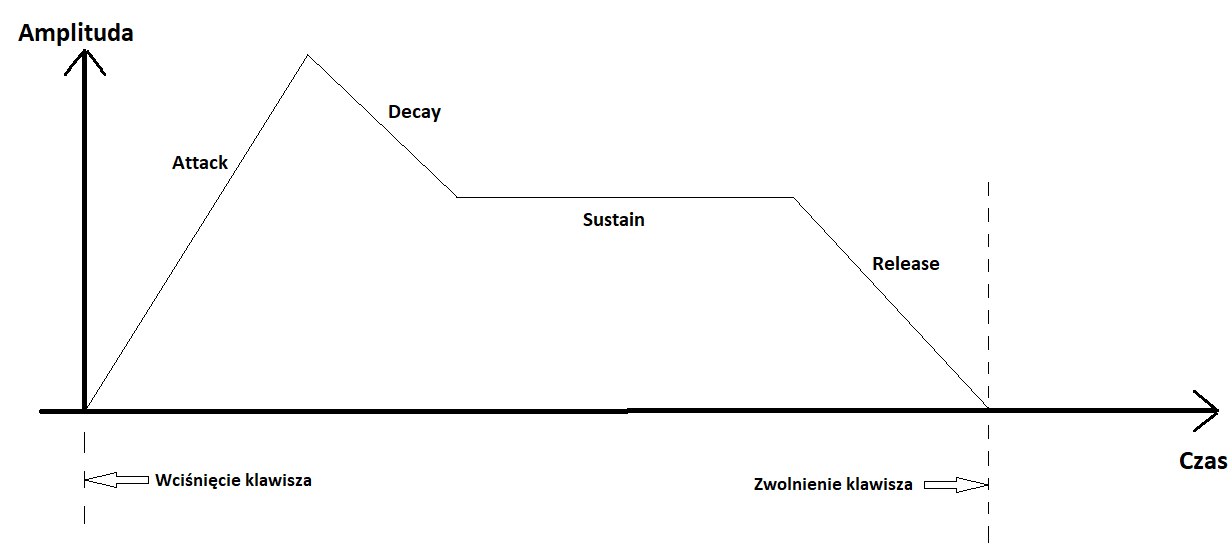
\includegraphics[width=12cm]{./grafiki/ADSR2}
	\captionsetup{justification=centering}
	\caption{Generator obwiedni dźwięku (ADSR).}
	\label{rys:ADSR}
\end{figure}

Na rysunku \ref{rys:ADSR} przedstawiono przykładową obwiednie dźwięku. Poniżej wytłumaczone zostały kolejne etapy ADSR:
\begin{enumerate}
	\item Attack - czas narastania amplitudy od zera do maksimum, rozpoczyna się, gdy klawisz zostaje naciśnięty.
	
	\item Decay - czas opadania amplitudy od maksymalnej wartości do poziomu podtrzymania dźwięku.
	
	\item Sustain - poziom amplitudy przy podtrzymaniu dźwięku. Trwa dopóki klawisz nie zostanie puszczony.
	
	\item Release - czas opadania amplitudy dźwięku od poziomu wyznaczonego przez etap Sustain do wartości zero.
\end{enumerate}
Moduł ADSR może być używany niezależnie od metody syntezy dźwięku.

\section{Analogowa i cyfrowa synteza dźwięku}
Debata na temat tego, który rodzaj syntezatorów jest lepszy, trwa od samego wprowadzenia cyfrowych syntezatorów (CS) do sprzedaży. Argumenty za i przeciw obu stron tego konfliku zazwyczaj odnoszą się do charakteru brzmienia obu rodzajów syntezatorów. Nie jest to jednak jedyna właściwość syntezatorów poróżniająca obie strony.

% Porownanie: https://www.synthtopia.com/content/2019/01/11/analog-vs-digital-synthesizer-blind-test/  W opisie na YT sa wyniki
Lorenzo Furlanetto utworzył test ślepego porównania (ang. blind test) klasycznego analogowego syntezatora (AS) oraz jego cyfrowej emulacji \cite{synthtopia}. Wyniki testu pokazały, iż 51 procent ankietowanych rozpoznało, który z syntezatorów był analogowy, natomiast aż 57 procent osób orzekło, iż dźwięk CS jest przyjemniejszy. Oznacza to, że trudno jest odróżnić dźwięk obu typów syntezatorów, oraz że większość słuchaczy preferuje brzmienia cyfrowe.

% https://blog.andertons.co.uk/labs/hardware-synths-vs-software-synths
Syntezatory cyfrowe, w stosunku do analogowych, posiadają wiele zalet. Za pomocą tych pierwszych można dokonać syntezy wielu rodzajów dźwięków, w tym również takich, które imitują brzmienia prawdziwych instrumentów. Analogowe syntezatory natomiast, pozwalają jedynie na uzyskanie prostych brzmień, za pomocą filtracji i zmian podstawowej grupy przebiegów (trójkątnych, prostokątnych, sinusoidalnych i piłokształtnych). 
Przewaga CS uwydatnia się szczególnie w przypadku łączenia wielu instrumentów cyfrowych i jednoczesnym wykonywaniu dźwieków za pomocą jednej klawiatury \cite{andertons}.

% zrobić skróty CS (cyfrowy syntezator) i AS (analogowy syntezator)

Z technicznego punktu widzenia, CS pozwalają również na wykorzystanie w procesie generacji dźwięku cyfrowych metod przetwarzania sygnałów. Parametry na przykład filtrów cyfrowych lub innych algorytmów nie ulegają degradacji z czasem, jak również można uzyskiwać ich charakterystyki o dowolonych kształach. Natomiast elementy składowe analogowych syntezatorów należy wymieniać lub dostrajać.

% +pamięć ustawien - łatwa konfiguracja
% pamięć RAM - nowe mozliwosci generowania sygnałów
% sampling
% nowe metody syntezy

\section{MIDI}
Cyfrowy interfejs instrumentów muzycznych (MIDI) to standard utworzony w 1983 roku, służący do przekazywania informacji pomiędzy cyfrowymi instrumentami muzycznymi. Zrewolucjonizował on sektor muzyki elektronicznej. Dzięki wdrożeniu tego protokołu, muzycy mogli używać na scenie jednej klawiatury muzycznej podłączonej do wielu modułów dźwiękowych, co nie było możliwe w erze syntezatorów analogowych. MIDI zawiera zarówno standard warstwy sprzętowej, jak i zestaw komend służących do komunikacji pomiędzy urządzeniami.

\subsection{Warstwa sprzętowa MIDI}
W interfejsie MIDI, informacje przesyłane są za pomocą szeregowego połączenia dwóch urządzeń cyfrowych, w trybie półdupleks. Szybkość przesyłu informacji została ustandardyzowana i wynosi 31250 bitów na sekundę \cite{dokumentacja_midi}. 
Podobnie jak w popularnym interfejsie UART, początek transmisji ramki danych rozpoczyna bit startu o wartości 0, natomiast kończy bit stopu o wartości logicznej jedynki. Interfejs MIDI jest interfejsem prądowym, gdzie logiczne zero oznacza przepływ prądu, natomiast logiczna jedynka oznacza brak jego przepływu.

\begin{figure}[H]
	\centering
	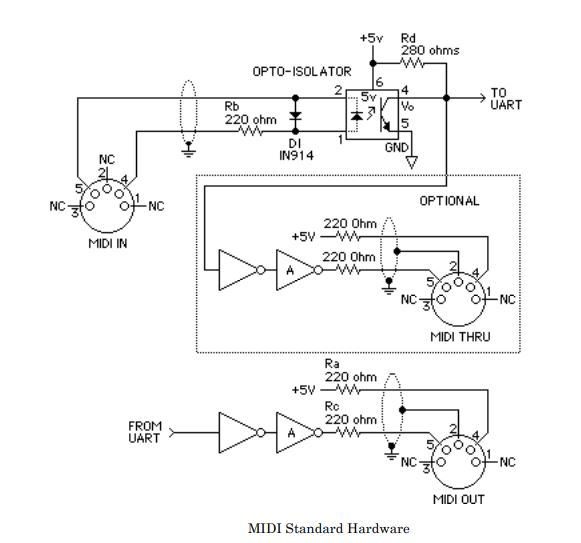
\includegraphics[width=9cm]{./grafiki/hardware_midi}
	\captionsetup{justification=centering}
	\caption{Schemat elektryczny interfejsu MIDI \cite{dokumentacja_midi}.}
	\label{rys:hardware_midi}
\end{figure}

Schemat sprzętowy interfejsu MIDI, znajdującego się po stronie instrumentu cyfrowego, przedstawiono na rysunku \ref{rys:hardware_midi}. Do połączeń z instrumentem używane są wtyki DIN pięciopinowe. Na wejściu interfejsu MIDI zawsze umieszczony zostaje transoptor, który chroni instrument otrzymujący informację przed uszkodzeniem.

\subsection{Protokół MIDI}
%https://www.midi.org/specifications-old/category/midi-1-0-detailed-specifications
%PDF: D:\Data\Studia\Magisterka\Literatura wstepna\MIDI
Wiadomości MIDI składają się z jednego bajta statusu, po którym następuje zazwyczaj jeden lub dwa bajty danych. Istnieją różne typy wiadomości MIDI. Dzieli się je na wiadomości kanałowe (odnoszące się do jednego kanału) oraz systemowe (odnoszące się do wszystkich kanałów). Wiadomości kanałowe mogą dzielić się dalej na komunikaty trybu lub komunikaty głosu. Te drugie w~praktyce stanowią większość przesyłanych komunikatów w transmisji MIDI.
Komunikat głosu może nieść informację na przykład o: naciśnięciu klawisza, zwolnieniu klawisza, aftertouch (zmiana siły nacisku na klawisz, odnotowana po pewnym czasie od jego naciśnięcia), pitch bend (delikatna zmiana wysokości dźwięku). Protokół MIDI, w ramach transmisji bajta danych (komunikat głosu), może obsłużyć 128 wysokości dźwięków z jednego instrumentu. Poziom głośności, zależny od siły nacisku na klawisz, również może przyjąć jedną ze 128 wartości.

Oprócz przesyłu informacji między urządzeniami MIDI, występuje dodatkowo sygnał zegarowy MIDI (ang. MIDI Pulses), który pozwala na zsynchronizowanie kilku instrumentów, do wykonywania utworu w jednakowym tempie. Informacje zegarowe występują cyklicznie i zawsze posiadają tę samą wartość bitową.



\section{Dyskretna transformacja Fouriera}
%Technika cyfrowego przetwarzania sygnałów - A. Leśnicki
Jednym z najważniejszych narzędzi w dziedzinie cyfrowego przetwarzania sygnałów jest dyskretna transformata Fouriera (DFT). Jest to przekształcenie zdefiniowane dla skończonych sygnałów dyskretnych. Pozwala ono na transformację dyskretnego sygnału czasowego na próbki widma dyskretnego. Posiada ono również swój odpowiednik zwany IDFT, który pozwala na przekształcenie dyskretne odwrotne, z widma do sygnału czasowego \cite{lesnicki}.

\subsection{Definicja przekształcenia DFT}
%Technika cyfrowego przetwarzania sygnałów 262 strona - A. Leśnicki
Dyskretne przekształcenie Fouriera oraz odwrócone dyskretne przekształcenie Fouriera są kolejno przedstawione następującymi wzorami:
\begin{equation} \label{equ:dft}
\openup\jot
\begin{aligned}[t]
X[k] = \sum_{n=0}^{N-1} x[n]e^{-j\frac{2\pi k}{N}n} \\ 
\end{aligned}
\qquad\qquad % adjust to suit
\begin{aligned}[t]
k = 0, 1, 2, ..., N - 1 \\
\end{aligned}
\end{equation}
\begin{equation} \label{equ:idft}
\openup\jot
\begin{aligned}[t]
x[n] = \frac{1}{N}\sum_{k=0}^{N-1} X[k]e^{j\frac{2\pi n}{N}k}  \\  
\end{aligned}
\qquad\qquad % adjust to suit
\begin{aligned}[t]
 n = 0, 1, 2, ..., N - 1 \\
 \end{aligned}
\end{equation}
\begin{tabular}{ l l l l}
	gdzie: & $X[k]$ &  - & k-ta próbka widma dyskretnego sygnału, \\
	&	$x[n]$ & - &  n-ta próbka dyskretnego sygnału w dziedzinie czasu, \\
	&	$N$ & - &  liczba próbek sygnału poddanego przekształceniu Fouriera,\\
	&	$n$ & - &  próbki dyskretnego sygnału w dziedzinie czasu, \\
	&	$k$ & - &  próbki dyskretnego widma sygnału. \\
\end{tabular}

We wzorach (\ref{equ:dft}) i (\ref{equ:idft}) przyjęto indeksowanie asymetryczne. Zapis taki wybrano z uwagi na bardziej czytelną postać. W celu uproszczenia zapisu definicji DFT stosuje się współczynniki obrotu (ang. twiddle factors):
\begin{equation} \label{equ:twid_fact}
\openup\jot
\begin{aligned}[t]
	W_{N}^{kn} = e^{-j\frac{2\pi}{N}nk}  \\
\end{aligned}
\qquad\qquad % adjust to suit
\begin{aligned}[t]
   k, n = 0, 1, 2, ..., N - 1. \\
\end{aligned}
\end{equation}

Współczynniki obrotu ułatwiają obliczenia, dzięki ich prostej interpretacji graficznej. Interpretowane są one jako wskazy na wykresie kołowym. Każdy ze współczynników należy rozumieć jako liczbę $e^{-j\frac{2\pi}{N}}$ podniesioną do potęgi $k$ razy $n$. W celu uzyskania uproszczonego zapisu definicji należy również zapisać próbki widma i sygnału w postaci wektorowej:

\begin{equation} \label{equ:dft_wekt}
\openup\jot
\begin{aligned}[t]
\mathbf{X} = 
\begin{bmatrix} 
X[0] \\ X[1] \\ ... \\ X[N-1]
\end{bmatrix}
\end{aligned}
\qquad\qquad % adjust to suit
\begin{aligned}[t]
\mathbf{x} =  
\begin{bmatrix} 
x[0] \\ x[1] \\ ... \\ x[N-1]
\end{bmatrix}.
\end{aligned}
\end{equation}

Ze wzorów (\ref{equ:twid_fact}) i (\ref{equ:dft_wekt}) uzyskuje się uproszczony zapis definicji DFT:
\begin{equation} \label{equ:dft_upr}
	\mathbf{X} = [W_{N}^{kn}]\mathbf{x},
\end{equation}
\begin{equation} \label{equ:idft_upr}
\mathbf{X} = \frac{1}{N}[W_{N}^{-kn}]\mathbf{x}.
\end{equation}

\subsection{Właściwości przekształcenia DFT}
%Technika cyfrowego przetwarzania sygnałów 269 strona - A. Leśnicki
Transformata DFT posiada wiele właściwości, których zastosowanie ułatwia realizację przetwarzania sygnałów cyfrowych. W poniższej tabeli przedstawiono te, które wykorzystane zostały w niniejszej pracy.

\begin{table}[H]
	\caption{Wybrane właściwości przekształcenia DFT.}
	\centering
	\label{tab:dft_wlasc}
	\begin{tabular}{|c|c|c|}
		\hline 
		\textbf{Nazwa właściwości} & \textbf{sygnał z okresem N} & \textbf{widmo DFT z okresem N} 	\\
		\hline
		Okresowość					& $x[n] = x[n + N]$ 				& $X[k] = X[k + N]$ 				\\	\hline
		Superpozycja			& $a_{1}x_{1}[n] + a_{2}x_{2}[n]$			& $a_{1}X_{1}[k] + a_{2}X_{2}[k]$			\\	\hline
		Przesunięcie cykliczne w czasie			& $x[n-K]$			& $ W_{N}^{kK}X[k]$			\\	\hline
		Korelacja cykliczna (splot kołowy)		 				& $x[n]*y^{*}[n]$			& $X[k]Y^{*}[k]$			\\ 	\hline
	\end{tabular}
\end{table}
W środkowej kolumnie tabeli \ref{tab:dft_wlasc} przedstawiono sygnał w dziedzinie czasu, a w prawej kolumnie przedstawiono odpowiednik tego sygnału w dziedzinie czestotliwości dla różnych operacji matematycznych stosowanych często w dziedzinie cyfrowego przetwarzania sygnałów.

\subsection{Algorytm FFT}
%Technika cyfrowego przetwarzania sygnałów 292 strona - A. Leśnicki
Wyznaczenie widma dyskretnego bezpośrednio z definicji (\ref{equ:dft}) jest bardzo złożone obliczeniowo. Przy założeniu, że próbki sygnału poddanego przekształceniu są liczbami zespolonymi, do obliczenia DFT wymagane jest $N^{2}$ mnożeń zespolonych oraz $N(N-1)$ dodawań zespolonych.

W praktyce obliczenia DFT sygnału wykonuje się z wykorzystaniem bardzo efektywnego algorytmu szybkiej transformacji Fouriera (FFT, ang. Fast Fourier Transform). Algorytm został przedstawiony w 1965 roku przez Cooleya-Tukeya i zapoczątkował nowy rozdział w dziedzinie cyfrowego przetwarzania sygnałów. Algorytm FFT można stosować również do obliczenia transformacji odwrotnej IDFT.

%https://en.wikipedia.org/wiki/File:DIT-FFT-butterfly.png
%https://pl.qwe.wiki/wiki/Butterfly_diagram
\begin{figure}[H]
	\centering
	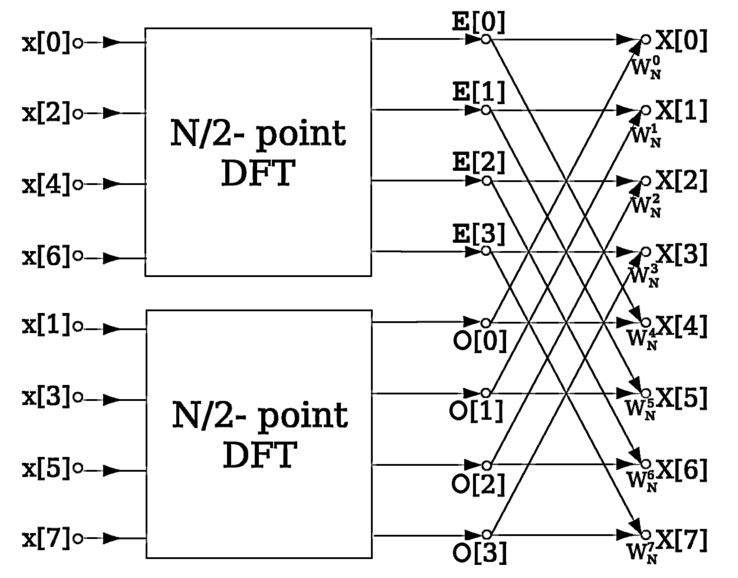
\includegraphics[width=8cm]{./grafiki/fft_motylki}
	\captionsetup{justification=centering}
	\caption{Algorytm FFT - schemat motylkowy.}
	\label{rys:fft_motyl}
\end{figure}

Algorytm FFT bazuje na metodzie dziel i zwyciężaj, dzieląc N-punktową transformację DFT na mniejsze transformacje N/2-punktowe, a następnie dokonując transformacji wyników poprzednich transformacji. Najbardziej popularną wersją algorytmu FFT jest FFT o podstawie 2, który wymaga $2^{k}$ próbek, gdzie k to liczba naturalna. Działanie algorytmu FFT o podstawie 2 opiera się na strukturach motylkowych i zostało przedstawione na rysunku \ref{rys:fft_motyl}.

%http://home.agh.edu.pl/~kkowal/DSP/FFT_wyklad.pdf
Dla liczby próbek $N$ równej $2^{k}$, występuje $log_{2}N$ poziomów algorytmu, a na każdym z nich jest $N/2$ operacji motylkowych. Ostatecznie złożoność obliczeniowa algorytmu FFT wynosi $\frac{N}{2}log_{2}N$. Pokazuje to, iż algorytm Cooleya-Tukeya jest zdecydowanie bardziej wydajny od obliczania DFT sygnału na podstawie definicji (\ref{equ:dft}).

	% !TeX spellcheck = pl_PL
\chapter{Realizacja instrumentu muzycznego}
Implementacja tworzonego syntezatora muzycznego realizowana jest na wspomnianej we wstępie płycie PADK, która opiera swoje działanie na procesorze DSP. W ramach tego implementowane jest wiele mechanizmów, które są konieczne do kompletnego działania projektu: przetwarzanie sygnałów z klawiatury muzycznej, wydobycie dźwięku z płyty PADK oraz komunikacja z interfejsem użytkownika. W niniejszym rozdziale przedstawiono podejście do realizacji wymienionych zadań. Implementacja poszczególnych algorytmów syntezy dźwięku przedstawiona zostanie w kolejnych rozdziałach.

Cały kod programu na procesor DSP napisany został w języku C. Program pisano w środowisku Code Composer Studio v6, które jest dedykowane do procesorów firmy Texas Instruments. Wgrywanie kodu na płytę odbywało się poprzez użycie debuggera XDS510 firmy Spectrum Digital. Debugger połączony jest z płytą PADK przez taśmę, a następnie przejściówkę 8-pinową.

% zdjęcie PADK z debuggerem

\section{Układ instrumentu}
% Zdjęcie i opis co z czym łączymy

\section{Płyta PADK}

\subsection{Procesor TMS320C6727}
%https://www.ti.com/lit/ds/symlink/tms320c6727.pdf?ts=1595978326019&ref_url=https%253A%252F%252Fwww.google.com%252F 
%--> glowne feature'y
%--> strona 13 wypisane w myslnikach np busy

\subsection{Peryferia komunikacyjne}

\subsection{Przetworniki DAC}



\section{Mechanizmy szybkiego przetwarzania danych}
Procesor sygnałowy TMS320C6727 jest przeznaczony między innymi do szybkiego przetwarzania danych i sygnałów. Poza wysoką szybkością taktowania procesora, firma Texas Instruments zawiera dodatkowe mechanizmy akceleracji przepływu danych i sygnałów. Zostały one opisane w poniższych podpunktach.

\subsection{McASP}
% https://www.ti.com/lit/an/sprack0/sprack0.pdf?ts=1595842361762&ref_url=https%253A%252F%252Fwww.google.com%252F
McASP to akronim od Multichannel Audio Serial Port. Jest to komunikacyjne urządzenie peryferyjne dedykowane do przetwarzania danych audio lub wideo. Został zaprojektowany w celu przypadków wymagających wielokanałowego przetwarzania dźwięku. Jedną z najbardziej przydatnych właściwości narzędzia McASP jest schemat wielozegarowy. Pozwala on na niezależność pomiędzy portami odbierającymi i nadającymi. Komunikacja, którą zarządza McASP może odbywać się poprzez interfejs I2S (ang. Inter-IC Sound), I2C (ang. Inter-Integrated Circuit) lub SPI (ang. Serial Peripheral Interface).

Kiedy dane przepływają przez McASP, mogą zostać dostosowane tak, aby reprezentacja stałoprzecinkowa używana przez kod aplikacji była niezależna od reprezentacji używanej przez urządzenia zewnętrzne, bez wymagania dodatkowej konwersji przez procesor.

W niniejszej pracy narzędzie McASP stosowane jest do przepływu danych między DAC a procesorem. W ramach inicjalizacji zegarów na płycie PADK, McASP ustawia odpowiednią szybkość próbkowania dla modułu DAC.

\subsection{dMAX}
%https://www.ti.com/lit/ug/spru795d/spru795d.pdf?ts=1595843361787&ref_url=https%253A%252F%252Fwww.google.com%252F, strona 14, Overview
Kontroler dMAX (Dual Data Movement Accelerator) obsługuje transfery zaprogramowane przez użytkownika pomiędzy kontrolerem pamięci wewnętrznej i urządzeniami peryferialnymi na procesorach DSP firmy TI. Mechanizm ten jest dedykowany szczególnie dla procesorów z serii C672x.

Zasada działania dMAX opiera się na sygnałach zdarzeń (ang. event signals). Zdarzenie zdefiniowane jest jako zmiana wartości logicznej odpowiadającego sygnału zdarzeń w rejestrze flag zdarzeń. Zdarzenie może być używane jako: wzbudzenie rozpoczęcia transferu danych lub spowodowanie wystąpienia przerwania dla CPU. Wszystkie zdarzenia posortowane są w dwie grupy: grupa niskiego priorytetu oraz grupa wysokiego priorytetu. Mechanizm dMAX może równolegle przetwarzać dwa żądania zdarzeń z każdej z grupy.

Częścią mechanizmu dMAX jest również bufor cyrkulacyjny FIFO. Pozwala on na równoczesny, asynchroniczny odczyt i zapis danych do jednego bufora dwustronnego. Narzędzie dMAX wykrywa kiedy dane zostają zapisane do bufora i natychmiastowo wywołuje odwrócenie go. Po odwróceniu, zapisane chwilę wcześniej dane mogą zostać odczytane z drugiej strony bufora, natomiast równocześnie kolejne dane zapisywane są po pierwszej stronie.


\section{Komunikacja z płytą PADK}
Do płyty PADK dołączone zostały dodatkowe biblioteki firmy Lyrtech, które ułatwiają obsługę komunikacji z płytą. Przykładem interfejsów, do których zostały utworzone nadmienione biblioteki to UART oraz MIDI.

\subsection{Komunikacja z klawiaturą muzyczną  (MIDI)}
% Datasheet "Professional Audio Development Kit Technical Reference Guide 1.4", September 2007
Jednym z podstawowych peryferiów klawiatury muzycznej jest wyprowadzenie interfejsu MIDI. Przeważnie jest to pięciopinowe gniazdo DIN. W płycie PADK zastosowano jednak dziewięciopinowe gniazdo typu D-sub. <do poprawy --> > Zatem wymagało to stworzenia odpowiedniego kabla, aby połączyć klawiaturę muzyczną z płytą PADK.
Do obsługi interfejsu MIDI wykorzystana została biblioteka PADK\_MIDI.c, która zawiera takie funkcje jak:
\begin{itemize}
	\item MIDI\_Init - inicjalizacja interfejsu MIDI,
	\item MIDI\_EnableLed1, MIDI\_EnableLed2 - sterowanie diodami LED interfejsu MIDI,
	\item MIDI\_Read - odczyt przychodzących bajtów. 
\end{itemize}
Aby w jak najmniejszym stopniu obciążać procesor, obsluga interfejsu MIDI została sprowadzona jedynie do odczytywania przychodzących bajtów poprzez przerwania sprzętowe.
Jako że ramki MIDI składają się z trzech bajtów, odczytywać oraz interpretować należy kolejne 3 przychodzące bajty.
Można to osiągnąć poprzez umieszczenie funkcji MIDI\_Read z parametrem 3 (odczyt 3 bajtów za jednym razem) w obsłudze przerwania. Jednak sytuację nieco komplikuje zegar MIDI, który powoduje, że DSP będzie odczytywał regularnie bajt o wartości 0xF8. Powoduje to, że w odczytanej sekwencji 3 bajtów pojawiała się niepożądana wartość 0xF8.
\begin{figure}[H]
	\centering
	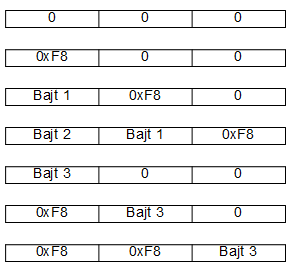
\includegraphics[width=8cm]{./grafiki/real_nofifo}
	\captionsetup{justification=centering}
	\caption{Odczytywane ramki MIDI przy braku odpowiedniej procedury odczytu.}
	\label{rys:real_nofifo}
\end{figure} 
Problem ten został zobrazowany na rysunku \ref{rys:real_nofifo}. Przedstawia on zawartość bufora wejściowego w czasie biegnącym od góry do dołu rysunku. W pokazanej sytuacji pomiędzy wywołaniem funkcji MIDI\_Read z parametrem 3, a nadejściem 3-bajtowej ramki danych, został odczytany bajt zegarowy. Ostatecznie odczytana zostanie ramka 4. oraz 7. od góry.  Oznacza to, że bajty, które miały zostać odczytane jako jedna ramka, mogą być dowolnie rozbite pomiędzy dwie obsługi przerwania. 
Aby rozwiązać ten problem, funkcja osbługi przerwania wywołuje funkcję MIDI\_Read z parametrem 1. W rezultacie kżdy przychodzący bajt wywołuje przerwanie. W obsłudze przerwania sprawdzana jest wartość bajta, jesli jest ona różna od 0xF8 (zegar MIDI), to zostaje ona dodana do trzyelementowej kolejki FIFO. W momencie gdy kolejka FIFO się zapełnia, ramka jest identyfikowana i interpretowana, a kolejka czyszczona. Działanie takiej kolejki zobrazowane jest na rysunku \ref{rys:real_fifo}.
\begin{figure}[H]
	\centering
	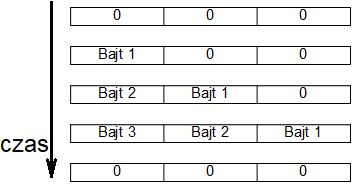
\includegraphics[width=8cm]{./grafiki/real_fifo}
	\captionsetup{justification=centering}
	\caption{Odczytywane ramki MIDI przy wykorzystaniu kolejki FIFO.}
	\label{rys:real_fifo}
\end{figure} 
Dzięki sprawdzaniu każdego przychodzącego bajta w obsłudze przerwania, do kolejki FIFO dostają się tylko istotne bajty. Dyskryminowanie wartości 0xF8 nie powinno mieć skutków ubocznych, gdyż wartość ta nie pojawia się w żadnym z bajtów ramki MIDI, poza bajtem statusu komunikatu zegarowego.
\subsection{Komunikacja z interfejsem użytkownika (UART)}
Do komunikacji z interfejsem użytkownika działajacym na komputerze klasy PC wykorzystany został interfejs RS-232, który znajduje się na płycie PADK. Do komunikacji z komputerem użyto przejściówki z RS-232 na USB. 
Do obsługi interfejsu szeregowego wykorzystana została biblioteka PADK\_UART.c, która zawiera takie funkcje jak:
\begin{itemize}
	\item UART\_Init - inicjalizacja interfejsu UART,
	\item UART\_EnableLed1, UART\_EnableLed2 - sterowanie diodami LED interfejsu UART,
	\item UART\_Read - odczyt przychodzących bajtów,
	\item UART\_Write - nadanie bajtów.
\end{itemize}
Aby zapewnić wygodny w użyciu oraz odporny na błędy przepływ informacji, utworzono własny protokół.
\begin{figure}[H]
	\centering
	
\includegraphics[width=16cm]{./grafiki/real_uartframe}
	\captionsetup{justification=centering}
	\caption{Struktura ramki protokołu.}
	\label{rys:real_uartframe}
\end{figure}
Na rysunku \ref{rys:real_uartframe} pokazana została struktura 9-bajtowej ramki danych, która jest przesyłana między DSP a komputerem. Składa się ona z dwóch bajtów identyfikujących, sześciu bajtow danych oraz jednego bajta sumy kontrolnej. Podobnie jak w przypadku MIDI, do identyfikacji i interpretacji przychodzących ramek, wykorzystywana jest kolejka FIFO. Tym razem ma ona rozmiar 9 bajtów. Bajty przychodzące są odczytywane pojedynczo przy wykorzystaniu przerwania sprzetowego i wpisywane do kolejki FIFO. W momencie gdy na pierwszym miejscu w kolejce znajdzie się odpowiedni bajt identyfikujący ramkę, a na miejscu ósmym znajdzie się wartość tego bajta powiększona o jeden, to jest domniemanie, że odebrana została jakaś ramka danych. W ramach upewnienia się, dodatkowo obliczana jest suma kontrolna z bajtów danych. Gdy ramka przejdzie taką weryfikację, zostaje następnie przetworzona w zależności od informacji, które niesie. Opisany mechanizm działa zarówno na procesorze DSP, jak i na komputerze PC.
<<<<<<< HEAD
Takie dziewięciobajtowe ramki pozwalają na przesyłanie na przykład całych zmiennych 4-bajtowych lub jednocześnie trzech liczb 2-bajtowych. 
=======
Dziewięciobajtowe ramki pozwalają na przesyłanie całych zmiennych 4-bajtowych lub jednocześnie trzech liczb 2-bajtowych. 



>>>>>>> JS: McASP update
\section{Wydobycie dźwięku (DAC)}
% pamiętać o: odniesienie do dMAX z buforem cyrkulacyjnym



\section{Klawiatura polifoniczna}
<W trakcie implementacji - opisać ogólnie, i powiedziec ze dla kazdej metody to bedzie wyglądało trochę inaczej>



\section{Wykorzystanie algorytmu FFT}
%http://www.secs.oakland.edu/~ganesan/old/courses/CSE671SU08/CSE%20671%20Lab%204%20ANC%20Code/Lee's%20adaptive%20wiener%20filter/DSPF_sp_cfftr2_dit.h

%https://processors.wiki.ti.com/index.php/C674x_DSPLIB <--- funkcje dsp_lib

W pamięci ROM procesorów z serii TMS320C672x zostały umieszczone specjalnie zoptymalizowane biblioteki, dedykowane do szybkiego przetwarzania sygnałów cyfrowych. Skompilowane biblioteki zostały napisane w asemblerze w celu większej efektywności obliczeniowej. 

%https://www.ti.com/lit/an/spraas8/spraas8.pdf?ts=1596035199216&ref_url=https%253A%252F%252Fwww.google.com%252F
W naszym projekcie, użyta została biblioteka \emph{DSP Library} z procesora TMS320C6727, która posiada efektywne obliczeniowo funkcje takie jak: transformacja FFT, odwracanie macierzy lub operacja na wektorach. W celu zawarcia jej w projekcie z programem na DSP, należało zmodyfikować komende pliku linkera dodając do niej bibliotekę o nazwie \emph{c67xdsplibR.lib}. Dodatkowo zmieniono sekcje pamięci, tak aby linker został odpowiednio poinstruowany, do których obszarów pamięci powinien się odnieść. Do pełnej transformacji FFT użyto trzech funkcji z nadmienionej biblioteki: DSPF\_sp\_cfftr2\_dit(), DSPF\_sp\_icfftr2\_dif() oraz DSPF\_sp\_bitrev\_cplx().

\subsection{Funkcje zawarte w procesorze}
%http://software-dl.ti.com/jacinto7/esd/processor-sdk-rtos-jacinto7/latest/exports/docs/dsplib_c66x_3_4_0_0/docs/doxygen/html/dsplib_html/group___f_f_t.html
Funkcja DSPF\_sp\_cfftr2\_dit() odpowiada za przeprowadzenie algorytmu FFT radix-2 z decymacją w dziedzinie czasu dla liczb zmiennoprzecinkowych. Sygnał na wejściu powinien posiadać N liczb zespolonych ułożonych w tablicy kolejno w pary liczb rzeczywistych i urojonych. Jako drugi argument wejściowy funkcja przyjmuje tablicę współczynników obrotu dla FFT o długości N/2. Współczynniki obrotu utworzone zostają przez zestaw trzech funkcji udostępnionych na stronie producenta procesora. Funkcję zostały skopiowane do naszego projektu. %https://www.rose-hulman.edu/class/ee/yoder/ece581/TI%20library/C6700/dsplib/support/fft/tw_r2fft.c <-- twiddle factors
Według dokumentacji, opisywana funkcja może również zostać użyta do uzyskania transformaty odwrotnej poprzez zmianę kolejności współczynników obrotu, a na końcu podzielenie wynikowej transformaty przez N, czyli według wzoru \ref{equ:idft_upr}. Wyniki zastosowania funkcji DSPF\_sp\_cfftr2\_dit() jako odwrotnej transformacji okazały się błędne. W celu poprawienia wyników, zastosowano funkcję DSPF\_sp\_icfftr2\_dif(), która dedykowana jest konkretnie do odwrotnej transformacji DFT. Wykonuje ona algorytm FFT radix-2 z decymacją w dziedzinie częstotliwości. Po użyciu tej funkcji, wyniki były poprawne.

%http://software-dl.ti.com/jacinto7/esd/processor-sdk-rtos-jacinto7/latest/exports/docs/dsplib_c66x_3_4_0_0/docs/doxygen/html/dsplib_html/group___d_s_p_f__sp__bitrev__cplx.html
Za zamianę kolejności próbek w tablicy wynikowej otrzymanej z funkcji wykonującej algorytm FFT odpowiada funkcja DSPF\_sp\_bitrev\_cplx(). Zmiana kolejności elementów tablicy realizowana jest przez odczytanie indeksów tablicy jako liczb w postaci bitowej, a następnie dokonanie lustrzanego odbicia każdego indeksu z osobna (ang. bit-reverse). Jest to niezbędny krok do zrealizowania pełnego algorytmu FFT radix-2.

\subsection{Pełna realizacja algorytmu przekształcenia}
Pełne wykorzystanie algorytmu wymaga odpowiedniego ułożenia omówionych wyżej funkcji. W tym celu utworzono bibliotekę z dodatkowymi funkcjami, które wykonują pełne przekształcenie DFT za pomocą algorytmu DFT. Funkcje dostępne dla użytkownika to fft\_full() oraz ifft\_full(). Pierwsza z nich ustawia funkcję w kolejności:
\begin{enumerate}
	\item bitrev\_full() - generacja współczynników obrotu, przygotowanie próbek dla algorytmu FFT,
	\item DSPF\_sp\_cfftr2\_dit() - wykonanie algorytmu FFT radix-2 z decymacją w dziedzinie czasu,
	\item DSPF\_sp\_bitrev\_cplx() - zmiana kolejności próbek po wykonaniu funkcji FFT,
\end{enumerate}
i pozwala na wykonanie pełnego przekształcenia prostego DFT. Druga natomiast, wykorzystuje funkcje:
\begin{enumerate}
	\item DSPF\_sp\_bitrev\_cplx() - generacja współczynników obrotu, przygotowanie próbek dla algorytmu FFT,
	\item DSPF\_sp\_icfftr2\_dif() - wykonanie algorytmu FFT radix-2 z decymacją w dziedzinie częstotliwości,
\end{enumerate}
do odwrotnego przekształcenia DFT.

% o rozdzielczości
% https://www.bitweenie.com/listings/fft-zero-padding/
\subsection{Dobranie dokładności FFT}
Jednym z wyzwań stawianych przed inżynierami zajmującymi się przetwarzaniem sygnałów za pomocą algorytmu FFT, jest odpowiednie dobranie ilości próbek do transformacji DFT. W związku z użyciem algorytmu FFT typu radix-2, ilość próbek musi być potęgą dwójki. Muzyczny charakter naszej pracy wymaga również wysokiej dokładności w dziedzinie częstotliwości, aby móc tworzyć tony o odpowiedniej częstotliwości. Miarą dokładności jest rozdzielczość algorytmu FFT, która określana jest wzorem:

\begin{equation} \label{equ:fft_resol}
\Delta R = \frac{f_{s}}{N_{fft}}
\end{equation}
\begin{tabular}{ l l l l}
	gdzie: 	&	$\Delta R$ & - &  rozdzielczość algorytmu FFT, \\
	&	$f_{s}$ & - &  częstotliwość próbkowania, \\
	&   $N_{fft}$ &  - & ilość punktów transformacji DFT. \\
\end{tabular}

% http://cds.cern.ch/record/720344/files/ab-note-2004-021.pdf
W literaturze można znaleźć informacje, iż widmo częstotliwościowe jest dużo bardziej czytelne i dokładne przy większej rozdzielczości algorytmu FFT. Minusem jej zwiększenia jest jednak spowolnienie obliczenia transformaty wynikowej i tym samym negatywny wpływ na czas pracy programu na procesorze.

%Potwierdzenie ze jak sie zwiekszy rozdzielczosc to jest lepiej https://ieeexplore-1ieee-1org-10000074b15d2.han.bg.pg.edu.pl/document/1604324
Podjęto próby osiągnięcia jak najlepszej rozdzielczości w realizowanym algorytmie FFT na procesorze TMS320C672x. Dokumentacja funkcji wskazywała, że maksymalna ilość próbek do transformacji powinna wynosić 2048. Niestety po wprowadzeniu takiej wartości, procesor ulegał zawieszeniu po chwili pracy. Po obniżeniu 


\section{Generowanie przebiegów czasowych}
% waveformy wykorzystywane w subtractive, additive oraz FM - dlatego opisywane tutaj


\section{ADSR}
<W trakcie implementacji>


\section{Interfejs użytkownika}
<TODO>
	\chapter{Subtraktywna metoda syntezy dźwięku}\label{chapter_subtractive}
\section{Zasada działania syntezy subtraktywnej}
Metoda subtraktywna polega na wygenerowaniu przebiegu okresowego bogatego pod względem składowych harmonicznych. Taki sygnał poddaje się filtracji w celu wytłumienia części składowych, co prowadzi do uzyskania interesujących dźwięków. Najczęściej wykorzystywanymi przebiegami w tej metodzie są: prostokątny, trójkątny, piłokształtny. Do usuwania składowych harmonicznych można zastosować filtry dolnoprzepustowe, górnoprzepustowego, pasmo-zaporowe czy pasmo-przepustowe. Na rysunku \ref{rys:sub_diagram} pokazano schemat blokowy opisanego postępowania.

\begin{figure}[H]
	\centering
	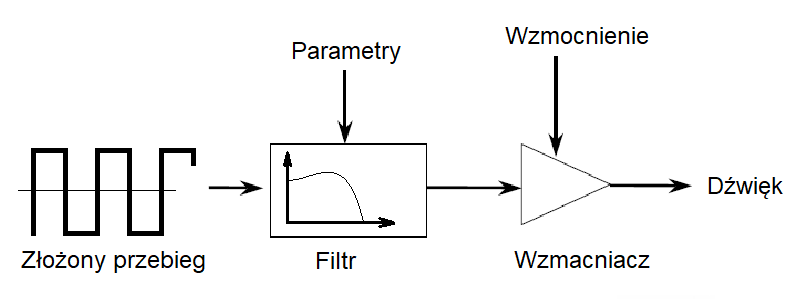
\includegraphics[width=12cm]{grafiki/sub_diagram}
	\captionsetup{justification=centering}
	\caption{Schemat blokowy dla metody subtraktywnej.}
	\label{rys:sub_diagram}
\end{figure}

Przykładowy wynik takiego działania przedstawiony jest na rysunku \ref{rys:sub_wykres1}.
\begin{figure}[H]
	\centering
	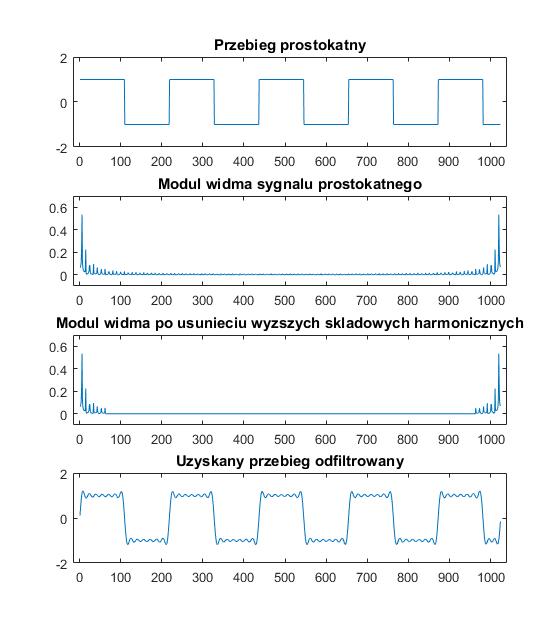
\includegraphics[width=12cm]{grafiki/sub_wykres1}
	\captionsetup{justification=centering}
	\caption{Zasada działania metody subtraktywnej.}
	\label{rys:sub_wykres1}
\end{figure}
Jak widać na \ref{rys:sub_wykres1}, na początku generowane jest 1024 próbek przbiegu prostokątnego. Następnie obliczane jest widmo tego sygnału. Z widma usuwane są wyższe składowe harmoniczne. Działanie to odpowiada filtracji idealnym filtrem dolnoprzepustowym. Z takiego widma, za pomocą odwrotnej transformacji Fouriera, obliczany jest przebieg czasowy. W wyniku otrzymuje się sygnał prostokątny po filtracji dolnoprzepustowej.
\section{Implementacja syntezy subtraktywnej}
W przypadku syntezatorów analogowych, poszczególne bloki są realizowane za pomocą elementów elektronicznych takich jak oscylatory (VCO) oraz przestrajalne filtry. W syntezatorach cyfrowych implementacje mogą być różne, jednak muszą być na tyle wydajne obliczeniowo, aby dana platforma sprzętowa poradziła sobie z syntezą dźwięku w czasie rzeczywistym bez artefaktów dźwiękowych. W tym podrozdziale opisana zostanie obrana droga implementacji metody subtraktywnej na procesorze sygnałowym. 
Próbki sygnału są syntezowane w sposób blokowy. Blok danych składa się z $N=1024$ próbek.

\subsection{Generowanie przebiegu}
W tablicy o $N$ elementach przechowywane są kolejne próbki sygnału bogatego w wyższe składowe harmoniczne. Po dokonaniu filtracji i wystawieniu tych próbek na przetwornik cyfrowo-analogowy, w tablicy tej należy wygenerować kolejne 1024 próbek sygnału. Trzeba przy tym pamiętać o odpowiednim przesunięciu fazowym, tak aby zachować ciągłość pomiędzy kolejnymi blokami próbek wystawianych na przetwornik. Równanie \ref{equ:sub_1} opisuje sposób generowania przebiegu prostokątnego.
\begin{equation} \label{equ:sub_1}
waveform[i]=\left \{\begin{array}{ r l }
1, & \quad \text{$dla$ } sin(2\pi f\frac{k+i}{F_s}) > 0\\
-1, & \quad  \text{$dla$ } sin(2\pi f\frac{k+i}{F_s}) \leqslant 0
\end{array}
\right.
\end{equation}
\begin{tabular}{ l l l l}
	gdzie: & $waveform$ &  - & tablica zmiennych typu float, \\
	&	$f$ & - &  pożądana częstotliwość generowanego przebiegu, \\
	&	$F_s$ & - & częstotliwość próbkowania,\\
	&	$i$ & - &  licznik iteracji, $i$ = 1, 2, 3, ..., N,\\
	&	$k$ & - &  licznik bloków.\\
\end{tabular} \\ \\
Po wyznaczeniu każdego bloku próbek, zwiększany jest licznik bloków $k$:
\begin{equation} \label{equ:sub_2}
k = k_{old} + N.
\end{equation}
Na rysunku \ref{rys:sub_waveform_blocks} pokazano dwa kolejne bloki próbek wygenerowanego przebiegu prostokątnego. Dzięki odpowiedniemu przesunięciu fazowemu przebiegi te, po wystawieniu na przetwornik cyfrowo-analogowy, utworzą ciągły dźwięk - bez trzasków.
\begin{figure}[H]
	\centering
	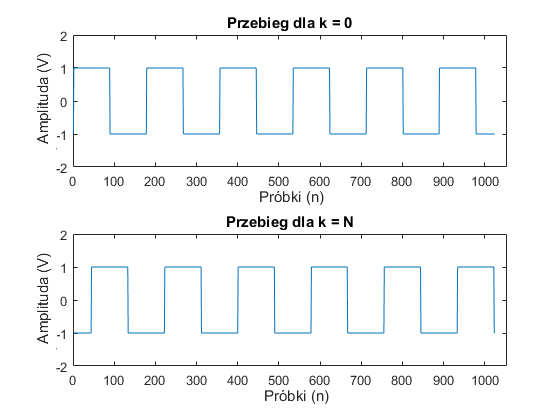
\includegraphics[width=12cm]{grafiki/sub_waveform_blocks}
	\captionsetup{justification=centering}
	\caption{Dwa kolejne bloki próbek przebiegu prostokątnego.}
	\label{rys:sub_waveform_blocks}
\end{figure}

\subsection{DFT i filtracja sygnału}
Na podstawie wygenerowanych próbek przebiegu oblicza się DFT za pomocą algorytmu FFT. W wyniku otrzymuje się $N$ liczb zespolonych. Przechowywane są one w tablicy o rozmiarze $2N$ w taki sposób, że każdy element o indeksie parzystym to część rzeczywista próbki, a sąsiadujący z nią element o indeksie nieparzystym to część urojona tej próbki. Filtracja dokonywana jest poprzez wyzerowanie elementów o odpowiednich indeksach. Na przykład filtracja dolnoprzepustowa z częstotliwością graniczną o wartości 1400 Hz dokonywana jest według poniżego wzoru:
\begin{equation} \label{equ:sub_3}
waveform_{fft}[i]=\left \{\begin{array}{ r l }
0, & \quad  \text{$dla$ } N - f_g \leqslant \frac{i}{2} \leqslant N + f_g \\
waveform_{fft}[i], & \quad \text{w pozostałych przypadkach } 

\end{array}
\right.
\end{equation}
\begin{tabular}{ l l l l}
	gdzie: & $waveform_{fft}$ &  - & próbki transformaty Fouriera sygnału, \\
	&	$freq$ & - &  częstotliwość przeliczona na indeksy w tablicy, $freq = N - 2 \frac{1400N}{Fs} - 1$, \\
	&	$F_s$ & - & częstotliwość próbkowania,\\
	&	$i$ & - &  indeks, $i$ = 1, 2, 3, ..., 2N.\\
\end{tabular} \\ \\

Efekt tego typu filtracji można zobaczyć na drugim i trzecim wykresie na \ref{rys:sub_wykres1}. W analogiczny sposób dokonuje się pozostałych filtracji: górnoprzepustowej, pasmo-przepustowej i pasmo-zaporowej.

\subsection{Zakładkowanie bloków danych}
Samo przesuwanie w fazie generowanych sygnałów opisanych w \ref{equ:sub_2} nie rozwiązuje wszystkich problemów. Jak widać na ostatnim wykresie na \ref{rys:sub_wykres1}, uzyskany sygnał na końcu ma niespodziewany przebieg. Po połączeniu tego bloku próbek z następnym blokiem otrzyma się sygnał pokazany na rysunku \ref{rys:sub_zakladkowania_brak}.
\begin{figure}[H]
	\centering
	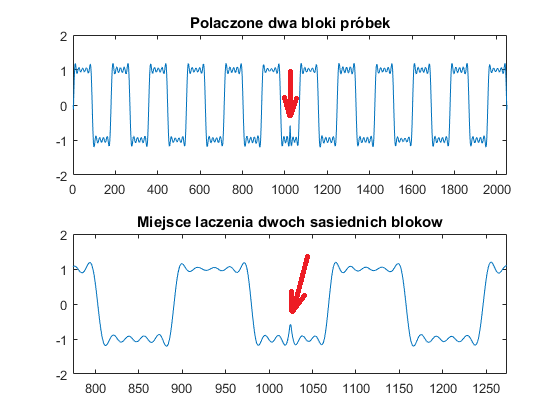
\includegraphics[width=12cm]{grafiki/sub_zakladkowania_brak}
	\captionsetup{justification=centering}
	\caption{Dwa kolejne bloki próbek przebiegu prostokątnego.}
	\label{rys:sub_zakladkowania_brak}
\end{figure}
Rozwiązaniem tego problemu jest zakładkowanie każdych dwóch sąsiednich bloków próbek. Zakładkowanie polega na nasunięciu pewnej liczby $m$ początkowych próbek następnego bloku, na $m$ końcowych próbek bieżącego. W miejscach, gdzie bloki są na siebie nałożone, wartość każdej próbki obliczana jest jako średnia ważona z dwóch nałożonych na siebie próbek. Przy czym suma wag w każdej chwili czasu jest równa 1, wagi próbek bloku bieżącego maleją wraz z czasem, natomiast wagi próbek bloku następnego narastają. Najprostszym rozwiązaniem (a zatem efektywnym obliczeniowo) są wagi liniowe. Oznacza to, że wagi dla $m$ ostatnich lub pierwszych próbek bloku odpowiednio: liniowo maleją od 1 do 0 lub liniowo rosną od 0 do 1.
Nakładane na siebie próbki muszą odpowiadać sygnałowi w tej samej fazie, zatem należy zmodyfikować przesunięcie fazowe opisane przez \ref{equ:sub_2} do postaci \ref{equ:sub_4}:
\begin{equation} \label{equ:sub_4}
k = k_{old} + N - m.
\end{equation}
Porównanie zakładkowania dla różnych wartości $m$ przedstawiono na \ref{rys:sub_overlaps}.
\begin{figure}[H]
	\centering
	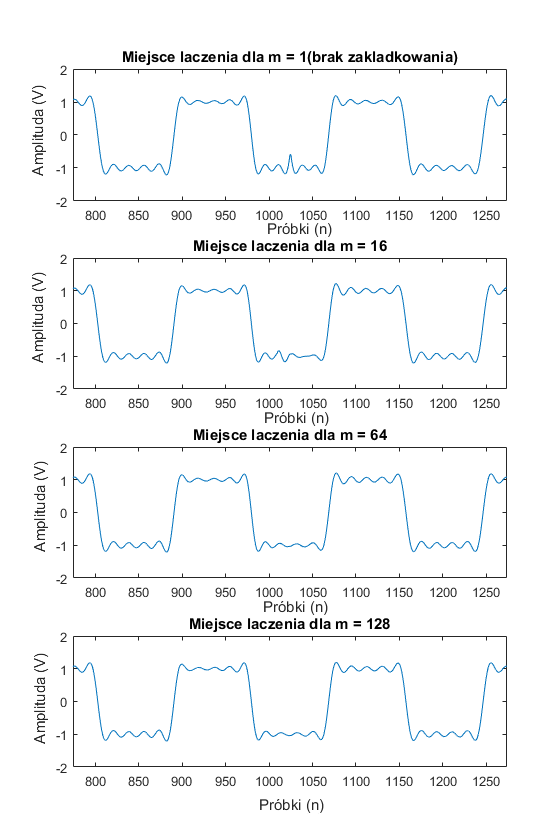
\includegraphics[width=10cm]{grafiki/sub_overlaps}
	\captionsetup{justification=centering}
	\caption{Wyniki zakladkowania przy zmiennej dlugosci zakladek.}
	\label{rys:sub_overlaps}
\end{figure}
siema
	\chapter{Addytywna synteza dźwięku}\label{chapter_additive}
Synteza addytywna pozwala na utworzenie barwy dźwięku poprzez zbudowanie pełnego widma częstotliwościowego za pomocą odpowiednich składowych. Słowo 'addytywna' odnosi się do sumowania wielu przebiegów w jeden złożony sygnał dźwiękowy. Historycznie jest ona drugą najstarszą metodą syntezy, zaraz po subtraktywnej, opisanej w rozdziale \ref{chapter_subtractive}.
Zazwyczaj synteza addytywna polega na dodawaniu wielu fal sinusoidalnych o różnych częstotliwościach oraz amplitudach. Metoda ta pozwala jednak na dużą dowolność. Dodawanymi składowywmi sygnału nie muszą być jedynie fale sinusoidalne.
Synteza addytywna uznawana jest za odwrotność syntezy subtraktywnej. Znajduje zastosowanie w syntezie dźwięku oraz mowy.

W niniejszym rozdziale przedstawiono zasadę działania syntezy addytywnej. Zaprezentowano wzory matematyczne, za pomocą których można uzyskać zsyntezowane brzmienie. Przedstawiono również kilka metod implementacji tego rodzaju syntezy. Na końcu rozdziału zaprezentowano autorski interfejs użytkownika oraz wyniki zaimplementowania syntezy addytywnej na procesorze DSP.

\section{Zasada działania syntezy addytywnej}
Synteza addytywna jest zbliżona pod niektórymi względami do analizy częstotliwościowej Fouriera. Z tego powodu jest ona zaliczana do widmowych metod syntezy. Jej postać matematyczną można jednak przedstawić w dziedzinie czasu. Zależnie od doboru składowych dźwięku, przedstawienie syntezy addytywnej może różnie wyglądać.
% Okresowosc sygnalu y(t)
%https://ccrma.stanford.edu/~jos/sasp/Additive_Synthesis_Early_Sinusoidal.html

\subsection{Postać harmoniczna} \label{pos_harm}
Dźwięk powstały w wyniku użycia syntezy addytywnej w formie harmonicznej można zapisać w postaci:
%https://en.wikipedia.org/wiki/Additive_synthesis#:~:text=Additive%20synthesis%20is%20a%20sound,or%20inharmonic%20partials%20or%20overtones.
\begin{equation} \label{equ:addit_time_harm}
y(t) = \sum_{k=1}^{K} a_{k}sin(2\pi kf_{0}t + \phi_{k})  \\  
\end{equation}
\begin{tabular}{ l l l l}
	gdzie: & $y(t)$ &  - & wyjście addytywnej syntezy dźwięku, \\
	&	$k$ & - &  numer składowej harmonicznej sygnału, \\
	&	$K$ & - &  całkowita liczba składowych harmonicznych dźwięku,\\
	&	$f_{0}$ & - &  częstotliwość pierwszej składowej harmonicznej,\\
	&	$a_{k}$ & - &  amplituda składowej harmonicznej k, \\
	&	$\phi_{k}$ & - &  faza składowej harmonicznej k. \\
\end{tabular} \\

Każda składowa dźwięku uzyskanego z tej postaci syntezy addytywnej jest wielokrotnością częstototliwości podstawowej $f_{0}$. Wykorzystanie takiej postaci pozwala na utworzenie dźwięku na przykład organów. Jest to najbardziej podstawowy rodzaj syntezy addytywnej.

%https://en.wikibooks.org/wiki/Sound_Synthesis_Theory/Additive_Synthesis <<---- SCHEMAT 

%https://en.wikipedia.org/wiki/Square_wave
\begin{equation} \label{equ:addit_sqr}
y_{Square}(t) = \sum_{k=1}^{K} \frac{1}{2k-1} sin(2\pi (2k-1)f_{0}t) \\
\end{equation}

%https://en.wikipedia.org/wiki/Triangle_wave
\begin{equation} \label{equ:addit_trng}
y_{Triangle}(t) = \sum_{k=1}^{K} \frac{(-1)^k}{(2k-1)^2} sin(2\pi (2k-1)f_{0}t)  \\
\end{equation}

%https://en.wikipedia.org/wiki/Sawtooth_wave
\begin{equation} \label{equ:addit_sawth}
y_{Sawtooth}(t) = \sum_{k=1}^{K} \frac{(-1)^k}{k} sin(2\pi kf_{0}t) \\
\end{equation}
% O tym że na tym polegały organy Hammonda

Postać harmoniczna syntezy addytywnej pozwala również na uzyskanie podstawowych przebiegów używanych w syntezie subtraktywnej. Każdy z nich można wygenerować za pomocą sumowania odpowiednich składowych harmonicznych z odpowiednimi amplitudami. Przykłady takich przebiegów przedstawiono we wzorach \ref{equ:addit_sqr}, \ref{equ:addit_trng} oraz \ref{equ:addit_sawth}.

\begin{figure}[H]
	\centering
	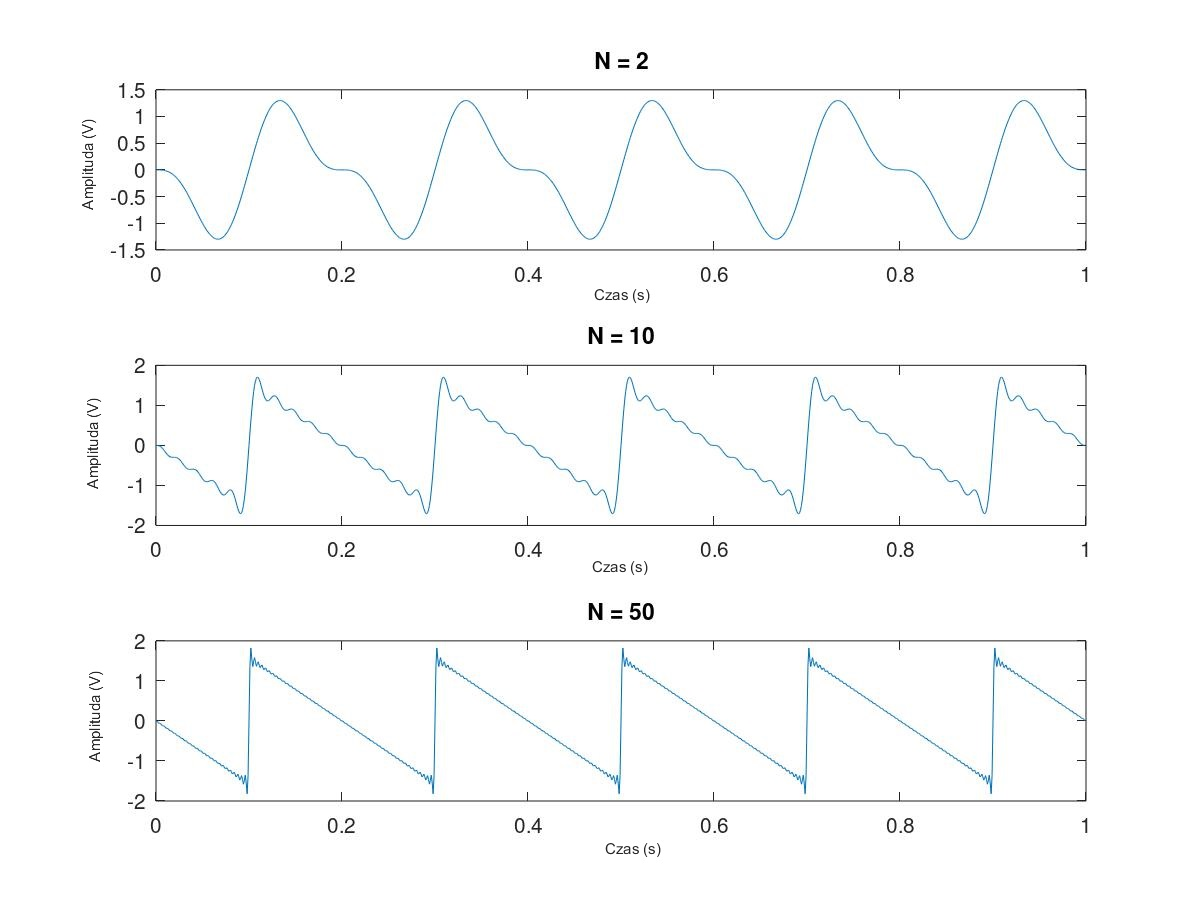
\includegraphics[width=12cm]{grafiki/add_sawtooth}
	\captionsetup{justification=centering}
	\caption{Generacja przebiegu piłokształtnego za pomocą syntezy addytywnej.}
	\label{rys:add_sawtooth}
\end{figure}

Na rysunku \ref{rys:add_sawtooth} przedstawiono wygenerowany przebieg piłokształtny, jako przykład addytywnej syntezy dźwięku w postaci harmonicznej. Na pierwszym z wykresów przedstawiono przebieg uzyskany z dwóch składowych harmonicznych, a na kolejnym z 10. Na ostatnim wykresie widać przebieg składający się z 50 SH, który jest dobrą aproksymacją idealnego przebiegu piłokształtnego. Amplitudy kolejnych składowych tego sygnału obliczone zostały na podstawie wzoru \ref{equ:addit_sawth}

\subsection{Postać nieharmoniczna} \label{pos_nieharm}
Dobieranie składowych dźwięku w syntezie addytywnej nie musi zależeć od konkretnej częstotliwości. Niektóre instrumenty wydają dźwięk składający się ze składowych harmonicznych i nieharmonicznych (czyli takich, które nie są całkowitą wielokrotnością pewnej częstotliwości $f_{0}$). Zsyntezowany dźwięk w takiej postaci można opisać wzorem:
\begin{equation} \label{equ:addit_time_nieharm}
y(t) = \sum_{k=1}^{K} a_{k}sin(2\pi f_{k}t + \phi_{k})  \\  
\end{equation}
\begin{tabular}{ l l l l}
	gdzie: 	&	$f_{k}$ & - &  częstotliwość składowej sygnału k,\\
\end{tabular} \\

Dźwięk opisany powyższym wzorem jest generowany przez instrumenty takie jak dzwony lub perkusjonalia.

\subsection{Składowe zmienne w czasie}
%https://books.google.pl/books/about/The_Computer_Music_Tutorial.html?id=nZ-TetwzVcIC&printsec=frontcover&source=kp_read_button&redir_esc=y#v=onepage&q&f=false
Wzory matematyczne \ref{equ:addit_time_harm} i \ref{equ:addit_time_nieharm} pozwalają na uzyskanie jedynie stanu ustalonego zsyntezowanego brzmienia. Powtarzany jest jeden okres sygnału, co daje wrażenie słuchaczowi, iż barwa dźwięku jest bardzo prosta.

Składowe dźwięku mogą jednak zmieniać się w czasie. Zmiany te mogą dotyczyć ich amplitudy, jak i częstotliwości.
Taką postać syntezy addytywnej zapisuje się:
\begin{equation} \label{equ:addit_time_zmienne}
y(t) = \sum_{k=1}^{K} a_{k}(t)sin(2\pi f_{k}(t)t + \phi_{k})  \\  
\end{equation}
\begin{tabular}{ l l l l}
	gdzie: & $a_{k}(t)$ &  - & zmienna w czasie amplituda składowej k, \\
	&	$f_{k}(t)$ & - &  zmienna w czasie częstotliwość składowej k, \\
\end{tabular} \\

\subsection{Szum w syntezie addytywnej}
%https://ccrma.stanford.edu/~jos/sasp/S_N_Synthesis.html
Tworzenie dźwięku zsyntezowanego metodą addytywną za pomocą wzorów przedstawionych powyżej jest deterministyczne. Do takiego sygnału można dodać jednak część stochastyczną. Uzyskuje się to z wykorzystaniem zmiennego w czasie filtra FIR oraz białego szumu.

\begin{equation} \label{equ:addit_szum}
B(\omega) = F(\omega)*e^{j\phi(\omega_{k})} \\  
\end{equation}
\begin{tabular}{ l l l l}
	gdzie: & $\phi(\omega_{k})$ &  - & faza losowa o rozkładzie równomiernym, \\
	& $F(\omega)$ &  - & obwiednia widmowa filtra FIR, \\
	&	$B(\omega)$ & - & zmienna w czasie częstotliwość składowej k, \\
\end{tabular} \\

Synteza części stochastycznej polega na przepuszczeniu białego szumu (bazującego na losowej fazie) przez filtr FIR. Takie działanie zostało zaprezentowane we wzorze \ref{equ:addit_szum}.
Dodanie szumu do sygnału deterministycznego w syntezie addytywnej pozwala na uzyskanie dźwięków na przykład instrumentów dętych.

\section{Metody implementacji syntezy addytywnej}

Istnieją różne metody implementacji addytywnej syntezy dźwięku. Ten sam dźwięk może być uzyskany różnymi sposobami. Popularne metody realizacji syntezy addytywnej to:
\begin{itemize}
	\item bank oscylatorów,
	\item synteza wavetable,
	\item synteza IFFT.
	% https://ieeexplore.ieee.org/document/4412805
\end{itemize}

\subsection{Ograniczenia syntezy addytywnej} \label{addit_ograniczenia}
%https://en.wikipedia.org/wiki/Additive_synthesis#History
Synteza addytywna w instrumentach klawiszowych jest używana między innymi do generacji dźwięku organów, których barwa upraszczana jest zazwyczaj do kilku SH. W przypadku próby uzyskania dźwięku o większej ilości składowych harmonicznych, złożoność obliczeniowa metody wzrasta.
%https://ccrma.stanford.edu/~jos/pasp/Additive_Synthesis.html
Przykładowo, dla uzyskania pojedynczego dźwięku pianina w jakości CD-Audio,
%https://en.wikipedia.org/wiki/Compact_Disc_Digital_Audio
wymagane byłoby obliczenie około 400 fal sinusoidalnych na każdą próbkę zsyntezowanego dźwięku. Oznacza to, iż dla polifonicznej klawiatury takiego pianina, byłyby to tysiące składowych. Obecne ograniczenia sprzętowe nie pozwalają na szybki rozwój addytywnej metody syntezy dźwięku, gdyż jest ona bardzo złożona obliczeniowo.

\subsection{Bank oscylatorów}
%analogowe hammondy i zwykłe, ale ze są wolne
Synteza przez bank oscylatorów jest najstarszą metodą implementacji addytywnej syntezy dźwięku. Opiera się ona bezpośrednio na równaniu \ref{equ:addit_time_harm}.
Ta metoda implementacji realizowana była nawet na instrumentach analogowych. Instrumenty takie jak organy Hammonda posiadały kilka dyskowych wirników, które były nacięte w kilku miejscach na ich powierzchni. Obracające wirniki generowały prąd elektryczny o charakterystyce zawierającej pewne składowe harmoniczne tonu podstawowego.

Implementacja na procesorach DSP, odpowiadająca dyskowym wirnikom, opiera się na realizowaniu wielu funkcji sin() o różnych częstotliwościach i amplitudach. Każda taka funkcja generuje jedną składową harmoniczną syntezowanego dźwięku. Wszystkie razem traktowane są jako bank oscylatorów. Problem realizacji skomplikowanego brzmienia takim sposobem został przedstawiony w punkcie \ref{addit_ograniczenia}.

\begin{figure}[H]
	\centering
	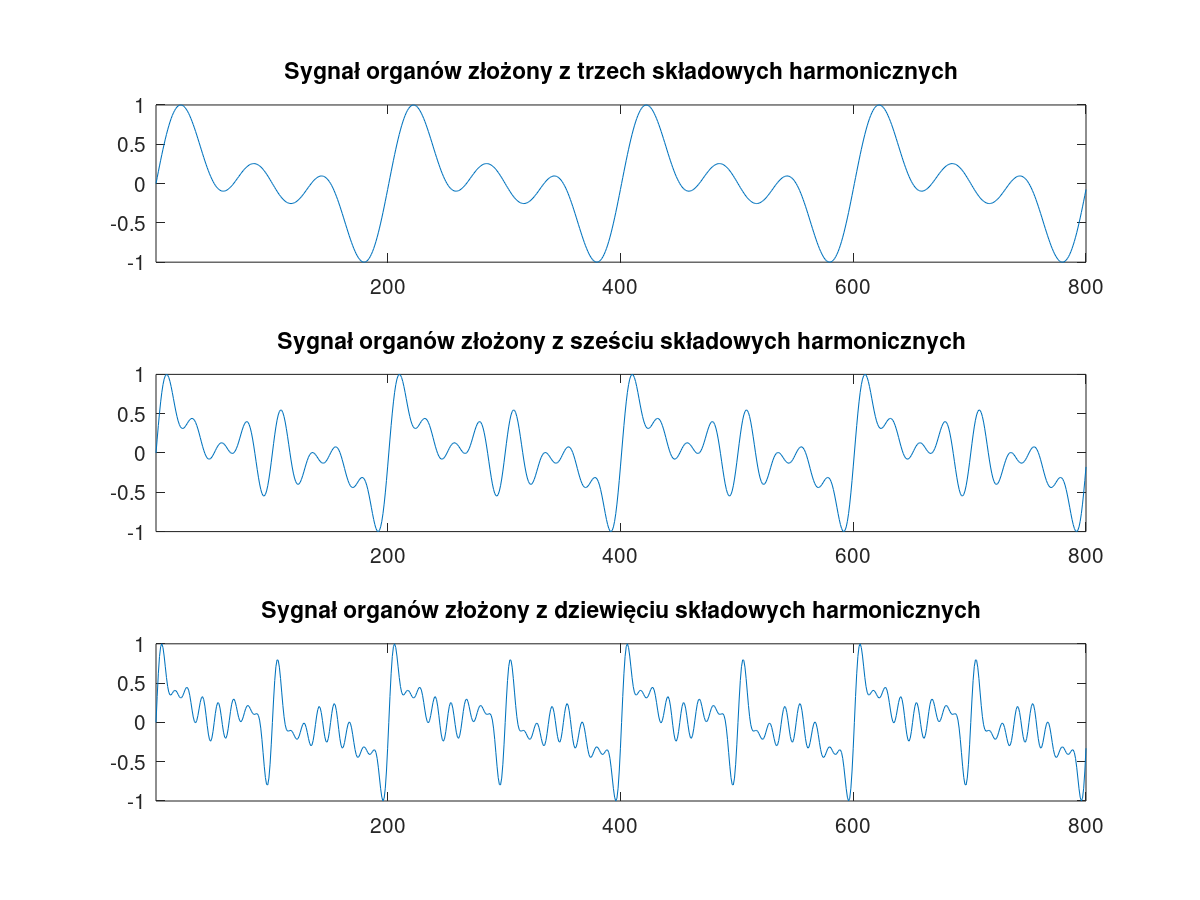
\includegraphics[width=15cm]{grafiki/add_hammond_matlab}
	\captionsetup{justification=centering}
	\caption{Barwa dźwięku organów Hammonda dla różnych ilości składowych harmonicznych.}
	\label{rys:add_hammond_matlab}
\end{figure}

Na rysunku \ref{rys:add_hammond_matlab} przedstawiono wygenerowaną barwę organów Hammonda dla trzech różnych ustawień amplitud składowych harmonicznych. Najbardziej zauważalna różnica występuje między pierwszym i ostatnim wykresem. Dodanie dziewięciu składowych harmonicznych bardzo zmienia charakter zsyntezowanego brzmienia w stosunku do sumowania jedynie trzech.


\subsection{Synteza wavetable} \label{add_wavetable}
%opisac tą która została zaimplementowana
Synteza wavetable (nazywana również syntezą tablicową lub lookup-table) polega na zapisaniu jednego okresu fali dźwiękowej do tablicy zdefiniowanej w programie komputerowym. W każdej kolejnej chwili czasu działania programu, odczytywany jest odpowiedni element tablicy. Okres fali zapisanej w tablicy powinien zawierać nadmierną liczbę próbek (ang. over-sampled), aby móc odczytać go dla niskich częstotliwościach. Niewystarczające spróbkowanie może doprowadzić do znacznych skoków wartości generowanej fali za pomocą metody wavetable.

W syntezie addytywnej użycie takiej metody implementacji może znacznie przyspieszyć generowanie kolejnych próbek składowych sygnału. Do tablicy zapisuje się jeden przebieg sinusoidalny. Odczyt jednego indeksu zabiera mniej czasu pracy procesora niż wygenerowanie próbki z funkcji sin(). Działanie takiej metody jest podobne do banku oscylatorów, ze względu na to, iż również realizowana jest w dziedzinie czasu. Znaczna różnica jest taka, że tablicę w syntezie wavetable można traktować jako jeden oscylator, z którego należy jedynie odczytać wartości tj. znaleźć odpowiedni indeks tablicy. Nie trzeba w każdej chwili czasu obliczać na nowo próbki dla każdej składowej dźwięku.
%https://en.wikipedia.org/wiki/Lookup_table

\subsection{Synteza IFFT}
%Rysunki z matlaba
W 1990 roku P. Depalle oraz X. Rodet przedstawili przełomową metodę implementacji syntezy addytywnej. W ich podejściu obliczanie składowych nie opiera się na zestawie oscylatorów, lecz na algorytmie IFFT (ang. Inverse Fast Fourier Transform) stosowanym dla krótkiego okna widma (STS, ang. short term spectrum). Wyniki ich pracy dowiodły, iż zmniejszyli koszt obliczeń syntezy addytywnej piętnastokrotnie, w stosunku do oscylatorów sinusoidalnych (w ich indywidualnym przypadku, gdzie obliczali 9 istotnych punktów widma w 256 próbkowym STS).

Konstrukcja pojedynczej ramki STS została przedstawiona poniżej. Niech $f_{j}$, $a_{j}$ oraz $\phi_{j}$ będą średnimi wartościami częstotliwości, amplitudy i fazy ramki czasowej pożądanego sygnału $w[n]$. $W$ niech będzie Transformatą Fouriera okna sygnału $w[n]$. Wtedy dodanie pojedynczej składowej do STS może być zapisana jako:

\begin{equation} \label{equ:addit_IFFT}
S[k] = a_{j}e^{i\phi_{j}}W[f_{j} - k] \\  
\end{equation}
\begin{tabular}{ l l l l}
	gdzie: & $S[k]$ &  - & STS syntezowanego sygnału, \\
	& $W[f_{j} - k]$ &  - & przesunięte widmo sygnału $w[n]$, \\
	& $a_{j}e^{i\phi_{j}}$ & - & zespolona amplituda. \\
\end{tabular} \\

Wzór \ref{equ:addit_IFFT} oznacza, iż okno widmowe $W[f_{j} - k]$ zostanie wycentrowane na częstotliwości $f_{j}$ oraz przemnożone przez amplitudę $a_{j}e^{i\phi_{j}}$. Po takim działaniu w dziedzinie częstotliwości, okno STS poddane jest algorytmowi IFFT, którego rezultatem jest okno czasowe $s[n]$. Kolejne okna czasowe zakładkowane są metodą overlap-add. Końcowo otrzymuje się pełen sygnał zsyntezowanego dźwięku za pomocą syntezy IFFT.

Dodanie szumu do sygnału jest również bardziej efektywne obliczeniowo w przypadku stosowanie takiej metody. Szum biały może zostać dodany już na etapie tworzenia STS, a następnie poddany algorytmowi IFFT. Ostatecznie uzyskiwane jest okno sygnału zawierającego część deterministyczną, jak i stochastyczną.

\section{Interfejs użytkownika}
W autorskim projekcie, w ramach realizacji instrumentu klawiszowego z syntezą addytywną, zaimplementowano program generujący dźwięk organów Hammonda. 
%https://www.soundonsound.com/techniques/synthesizing-tonewheel-organs-part-1
Laurens Hammond, twórca tychże organów, zaprojektował je tak, aby użytkownik miał możliwość doboru amplitudy dziewięciu składowych harmonicznych generowanego dźwięku. Każda z nich była regulowana suwakiem na 8 poziomach. Suwaki oznaczały kolejne wartości amplitudy pierwszej, drugiej, trzeciej, czwartej, szóstej, ósmej, dziesiątej, dwunastej oraz szesnastej składowej harmonicznej dźwięku. Przykładowe różnice w generowanej barwie organów przedstawione zostały na rysunku \ref{rys:add_hammond_matlab}.
\begin{figure}[H]
	\centering
	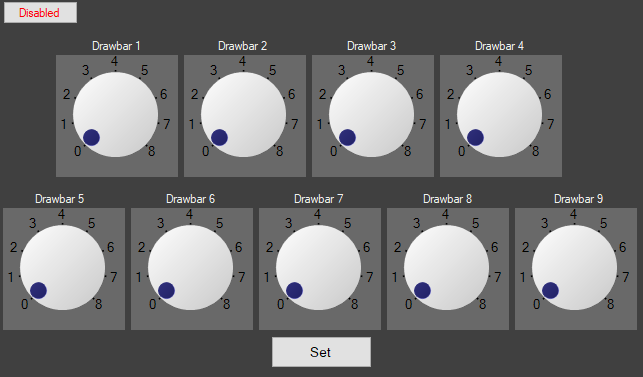
\includegraphics[width=15cm]{grafiki/add_interface}
	\captionsetup{justification=centering}
	\caption{Interfejs użytkownika dla syntezy addytywnej.}
	\label{rys:add_interface}
\end{figure}

Interfejs użytkownika opiera się na oryginalnym instrumencie Laurensa Hammonda. Umożliwia on użytkownikowi regulację dziewięciu SH za pomocą gałek przedstawionych na rysunku \ref{rys:add_interface}. Można zauważyć, iż gałki posiadają również 8 poziomów wartości, które odpowiadają wartościom amplitud składowych harmonicznych. Po ustawieniu pożądanej barwy, użytkownik musi kliknąć w panelu przycisk "Set", aby parametry syntezy addytywnej zostały wysłane do procesora DSP.

Gałki w panelu zostały zrealizowane za pomocą obiektów klasy KnobControl. Naciśnięcie przycisku "Set" wywołuje funkcję, która odczytuje wartość elementu panelu syntezy addytywnej w formie tablicy bajtów. Następnie wysyła odpowiedni identyfikator gałki do procesora DSP, a po nim jej wartość odczytaną z tablicy.

\section{Realizacja organów na procesorze DSP}
Pierwszym podejściem do implementacji organów Hammonda na procesorze DSP, było wykorzystanie banku oscylatorów. Rezultaty były jednak niezadowalające. Wywołanie funkcji sin() kilkukrotnie dla jednej próbki sygnału, oznaczało, iż w podejściu polifonicznym musiała ona zostać wywołana kilkadziesiąt razy.
Pomimo zastosowanego mechanizmu zakładkowania, w generowanym dźwięku pojawiały się niepożądane artefakty świadczące o zbyt dużej złożoności obliczeniowej zaimplementowanego algorytmu. Należało zmienić podejście do implementacji syntezy addytywnej.

Ostatecznie w autorskim programie komputerowym na procesor DSP wykorzystano metodę implementacji z użyciem tablicy wavetable, która została omówiona w punkcie \ref{add_wavetable}. W niniejszym rozdziale przedstawiony zostanie sposób realizacji programu umożliwiającego syntezę dźwięku organów Hammonda oraz rezultaty takiej syntezy na układzie TMS320C6727.

\subsection{Opis implementacji}
Tablica lookup o nazwie sinLut[.] zawiera jeden okres fali sinusoidalnej. Wypełniona zostaje na etapie inicjalizacji programu na procesorze DSP. Każdy element tablicy zostaje odczytany za pomocą funkcji mySin(), która jako argumenty przyjmuje częstotliwość pożądanej fali sinusoidalnej oraz jej przesunięcie w fazie.
\begin{equation} \label{equ:addit_sinLut}
\text{samp} = \text{sinLut}[(kf\frac{N}{F_s})\mod{N}] \\  
\end{equation}
\begin{tabular}{ l l l l}
	gdzie: & \text{samp} &  - & wartość próbki odczytywanej z tablicy sinLut[.], \\
	& $k$ &  - & licznik odczytu odpowiedniej próbki z tablicy sinLut[.], \\
	& $f$ & - & częstotliwość sinusoidy, \\
	& $N$ & - & długość tablicy sinLut[.], \\
	& $F_s$ & - & częstotliwość próbkowania DAC. \\
\end{tabular} \\

Funkcja mySin() zwraca element z tablicy na podstawie wzoru \ref{equ:addit_sinLut}. Do wygenerowania jednej próbki organów Hammonda sumowane jest 9 tak odczytanych wartości sinLut[.] (odpowiadających składowym harmonicznym). Każda próbka zsyntezowanego dźwięku ulega wymnożeniu z obecną wartością amplitudy ADSR. Opisana czynność wykonywana jest tyle razy, jaką ilość elementów posiada jeden blok generowanego sygnału.

Procesor DSP otrzymuje nastawy gałek syntezy addytywnej z interfejsu użytkownika w obsłudze przerwania UART. Parametry te są zapisywane do tablicy add\_knobAmp[.]. Następnie używane są do syntezy dźwięku organów.

\subsection{Wyniki}
Wykorzystana metoda implementacji za pomocą tablicy wavetable umożliwiła naciśnięcie nawet kilkunastu klawiszy bez pojawienia się niepożądanych artefaktów w dźwięku. Zmiany amplitud poszczególnych składowych harmonicznych wpływają na generowane w brzmienie w bardzo wyraźny sposób.

\begin{figure}[H]
	\centering
	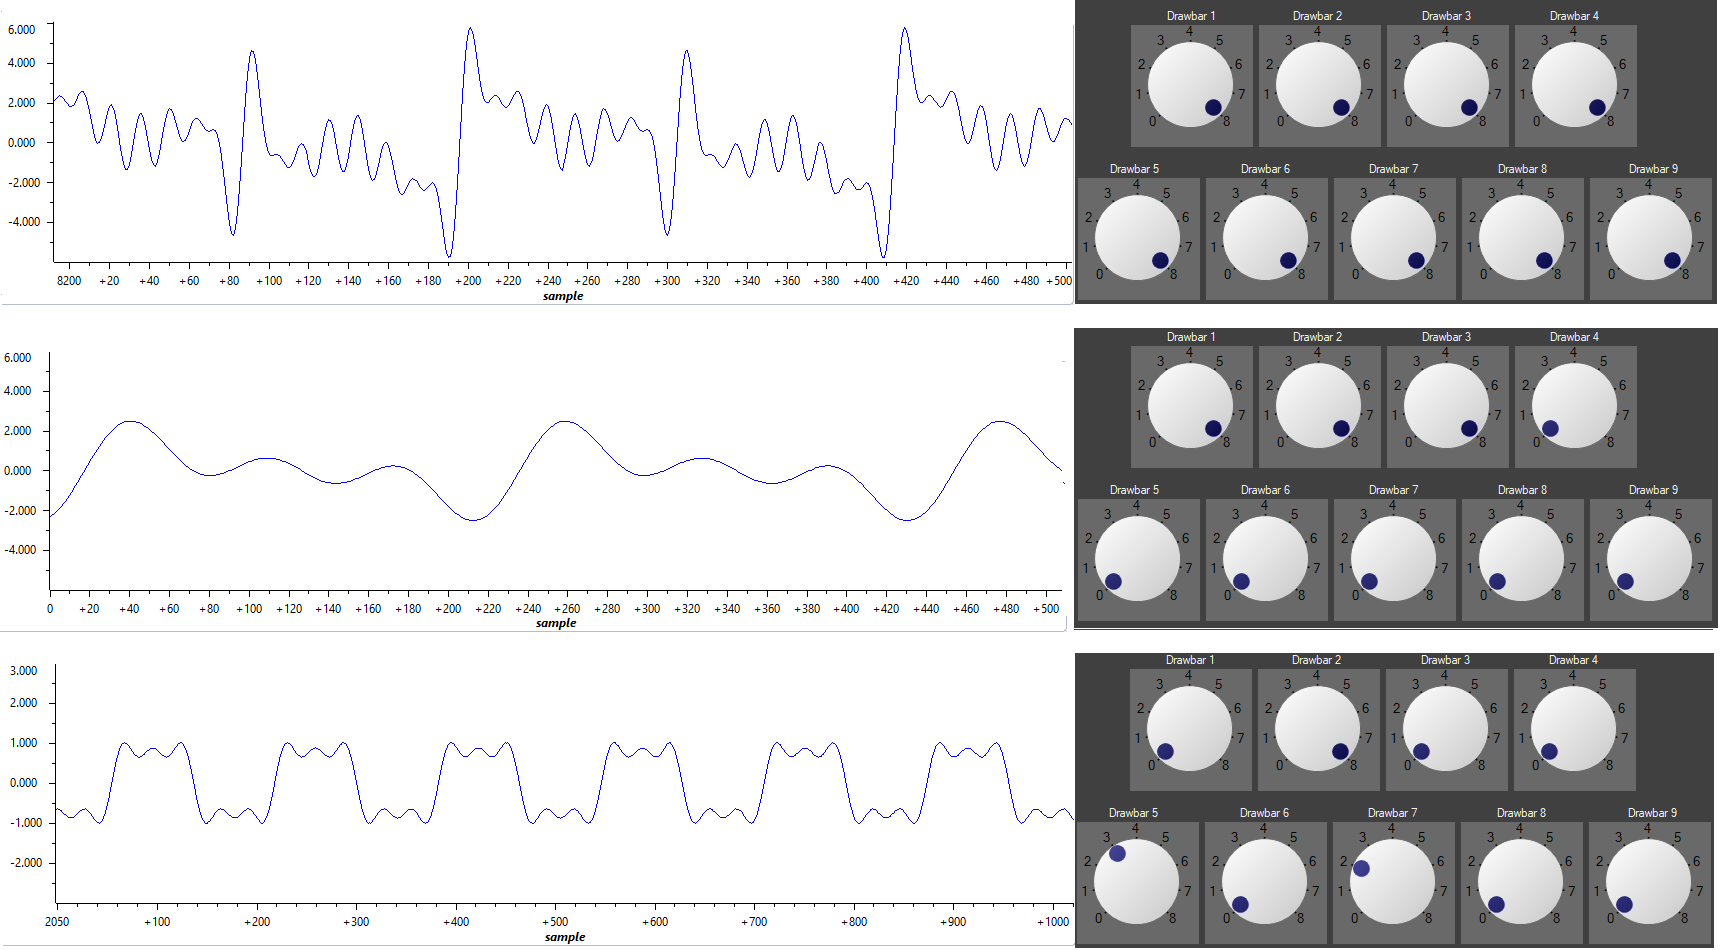
\includegraphics[width=15cm]{grafiki/add_hammond_dsp}
	\captionsetup{justification=centering}
	\caption{Wizualizacja sygnału dźwiękowego organów Hammonda z procesora DSP.}
	\label{rys:add_hammond_dsp}
\end{figure}

Na rysunku \ref{rys:add_hammond_dsp} przedstawiono wizualizację sygnału organów dla różnych ustawień gałek w interfejsie użytkownika. Na wykresie pierwszym od góry wszystkie SH mają maksymalną amplitudę (konfiguracja "8888 88888"). Tak wygenerowany dźwięk bardzo przypomina brzmienie katedralnych organów piszczałkowych. Na kolejnym wykresie przedstawiono sygnał utworzony przy konfiguracji gałek na wartościach "8880 00000". Brzmienie dźwięku przy takim ustawieniu gałek jest dużo bardziej delikatne niż w pierwszej konfiguracji. Na najniższym wykresie ustawienie amplitud to "0800 30200". Można zauważyć, iż wizualnie bardzo przypomina przebieg prostokątny. Brzmienie tak wygenerowanego dźwięku również jest zbliżone do dźwięku przebiegu prostokątnego.

Przedstawione barwy organów brzmiały by lepiej po dodaniu takich efektów jak Chorus lub Vibrato. Do uzyskania pełni brzmienia takich organów, często również stosuje się efekt pogłosu (ang. reverb).
	\chapter{Synteza dźwięku - modulacja częstotliwościowa}\label{chapter_fm}
Modulacja częstotliwościowa jest powszechnie kojarzona z radiem analogowym. W tym zastosowaniu, w chwilowej częstotliwości sygnału sinusoidalnego zaszyta jest informacja, która ma drogą radiową dotrzeć do odbiorcy. W przypadku syntezy dźwięku, modulowane są dowolne sygnały okresowe. Nie niosą one żadnej informacji, a dewiacje częstotliwości chwilowej wprowadza się w celu uzyskania wrażeń dźwiękowych.
\section{Zasada działania modulacji częstotliwościowej}
Modulacja częstotliwościowa polega na zmienianiu częstotliwości chwilowej przebiegu okresowego. Sygnał, którego częstotliwość ulega tym zmianom nazywany jest sygnałem modulowanym czy też nośnym. Zmiany wprowadzane w częstotliwości sygnału modulowanego, to odchylenia od jego własnej częstotliwości. Mogą one być dokonywane za pomocą innego sygnału okresowego, który nazywany jest sygnałem modulującym. 
\subsection{Modulacja FM w dziedzinie czasu}
Przykładem sygnału modulującego może być sinusoida. Przebieg zmodulowany częstotliwościowo, z pominięciem fazy sygnału modulującego \cite{oland}, opisuje wyrażenie:
\begin{equation} \label{equ:fm_wzor1}
S(t)= sin(2 \pi f_c t + \beta sin(2 \pi f_m t))
\end{equation}
\begin{tabular}{ l l l l}
	gdzie: & $t$ &  - & czas w sekundach, \\
	&	$f_c$ & - &  częstotliwość sygnału nośnego,\\
	&	$f_m$ & - &  częstotliwość sygnału modulującego.\\
	&	$\beta$ & - & amplituda sygnału modulującego.\\
\end{tabular} \\ \\
Na rysunku \ref{rys:fm_wykres1} zobrazowano modulację przeprowadzoną według (\ref{equ:fm_wzor1}) z parametrami: $\beta = 15, f_c = 1200, f_m = 55$.
\begin{figure}[H]
	\centering
	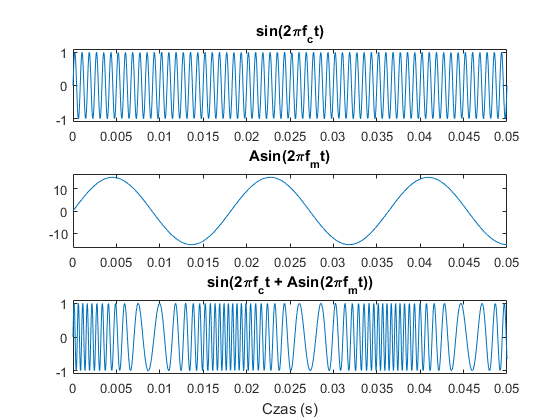
\includegraphics[width=12cm]{grafiki/fm_wykres1}
	\captionsetup{justification=centering}
	\caption{Prosty przykład sygnału zmodulowanego.}
	\label{rys:fm_wykres1}
\end{figure}
Na rysunku \ref{rys:fm_arg} przedstawiono przebiegi argumentów funkcji sinus z (\ref{equ:fm_wzor1}) dla pierwszych 50 milisekund sygnału.
\begin{figure}[H]
	\centering
	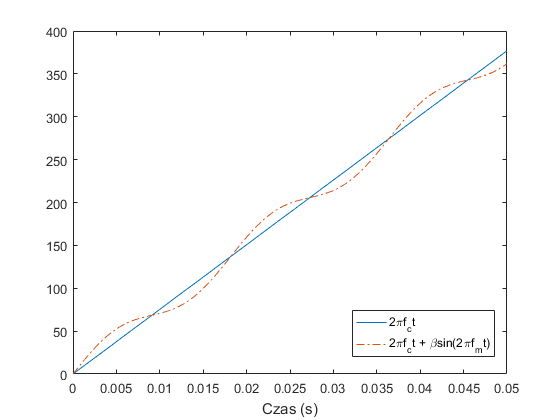
\includegraphics[width=10cm]{grafiki/fm_arg}
	\captionsetup{justification=centering}
	\caption{Przebiegi czasowe argumentu funkcji sinus przed i po modulacji FM.}
	\label{rys:fm_arg}
\end{figure}
Linią ciągłą narysowano przebieg argumentu sygnału nośnego przed modulacją. Natomiast linia przerywana obrazuje przebieg argumentu sygnału po modulacji częstotliwościowej.
\subsection{Modulacja FM w dziedzinie częstotliwości}
Wartość $\beta$ jest także określana mianem indeksu modulacji \cite{chowning}. Widmo sygnału poddanego modulacji częstotliwościowej składa się z prążka środkowego na częstotliwości nośnej oraz prążków bocznych. Prążki boczne są rozmieszczone symetrycznie względem częstotliwości nośnej i leżą na częstotliwościach $f_c \pm kf_m$, gdzie $k$ jest liczbą całkowitą. Moduł widma sygnału z powyższego przykładu przestawiony został na rysunku \ref{rys:fm_widmo}. Sygnał poddany transformacji Fouriera miał długość 96000 próbek przy $F_s = 96000$, zatem indeks częstotliwościowy jest równoważny częstotliwości. Ze względu na sposób indeksowania w Matlabie, zaczynający się od liczby 1 (a nie od 0), w celu uzyskania wartości częstotliwości należy odjąć jedynkę od indeksu.

\begin{figure}[H]
	\centering
	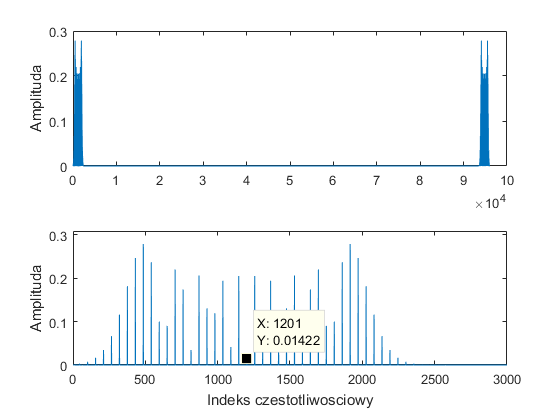
\includegraphics[width=10cm]{grafiki/fm_widmo}
	\captionsetup{justification=centering}
	\caption{Moduł widma sygnału zmodulowanego (wartość indeksu 1201 należy pomniejszyć o 1 ze względu na sposób indeksowania w Matlabie).}
	\label{rys:fm_widmo}
\end{figure}
Wraz ze wzrostem wartości $\beta$, wzrasta liczba znaczących prążków bocznych oraz poszerza się pasmo częstotliwościowe sygnału zmodulowanego.
Wartości poszczególnych prążków odpowiadają wartościom funkcji Bessela typu pierwszego $J_n(x)$, gdzie $n$ jest rzędem. Wykresy tych funkcji dla trzech pierwszych rzędów przedstawione są na rysunku \ref{rys:fm_bessel}.
\begin{figure}[H]
	\centering
	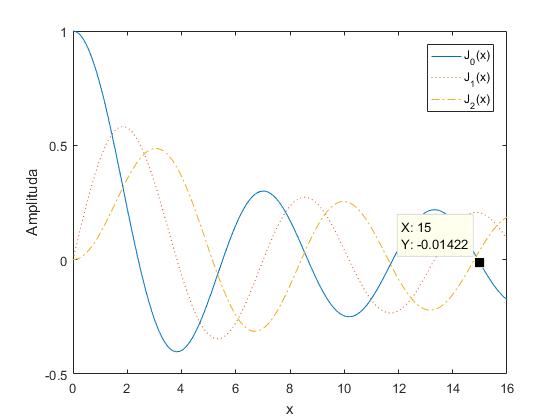
\includegraphics[width=10cm]{grafiki/fm_bessel}
	\captionsetup{justification=centering}
	\caption{Funkcje Bessela typu pierwszego.}
	\label{rys:fm_bessel}
\end{figure}

Moduł funkcji Bessela rzędu 0 w punkcie $\beta$ jest równy modułowi prążka na częstotliwości $f_c$. Moduł pierwszych prążków bocznych, tj. na częstotliwościach $f_c \pm f_m$ jest równy funkcji Bessela rzędu 1 w punkcie $\beta$. Postępując analogicznie można wyznaczyć moduły wszystkich znaczących prążków.

\subsection{Rozbudowana modulacja FM}
Zastosowanie modulacji FM w syntezie dźwięku ma doprowadzić do uzyskania wrażeń słuchowych. Zatem nic nie stoi na przeszkodzie, aby tę modulację rozbudowywać wedle własnego uznania. Można na przykład poddać modulacji przebieg modulujący. Niech sygnał modulujący (SM1) będzie modulowany przez SM2 (sygnał modulujący 2). Na rysunku \ref{rys:fm_modmod} przedstawiono wykresy sygnału nośnego, SM1, SM2 oraz sygnału końcowego, który jest opisany przez wzór:
\begin{equation} \label{equ:fm_modmod}
S(t)= sin(2 \pi f_c t + \beta sin(2 \pi f_m t + \gamma sin(2 \pi f_{m2} t)))
\end{equation}
\begin{tabular}{ l l l l}
	gdzie: & $t$ &  - & czas w sekundach, \\
	&	$f_c$ & - &  częstotliwość sygnału nośnego,\\
	&	$f_m$ & - &  częstotliwość SM1,\\
	&	$f_{m2}$ & - &  częstotliwość SM2,\\
	&	$\beta$ & - & amplituda SM1,\\
	&	$\gamma$ & - & amplituda SM2.\\
\end{tabular} \\ \\

\begin{figure}[H]
	\centering
	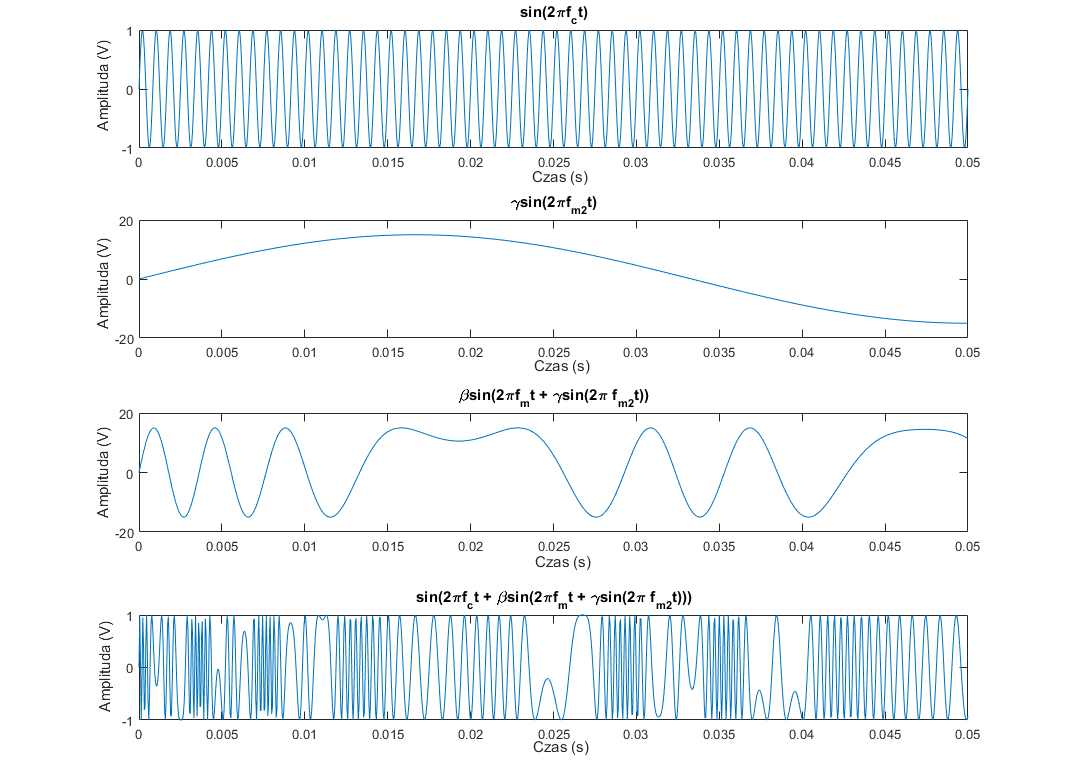
\includegraphics[width=14cm]{grafiki/fm_modmod}
	\captionsetup{justification=centering}
	\caption{Zagnieżdżona modulacja FM.}
	\label{rys:fm_modmod}
\end{figure}
Na rysunku \ref{rys:fm_arg2} przedstawiono przebiegi argumentów funkcji sinus z (\ref{equ:fm_modmod}) dla pierwszych 50 milisekund sygnału.
\begin{figure}[H]
	\centering
	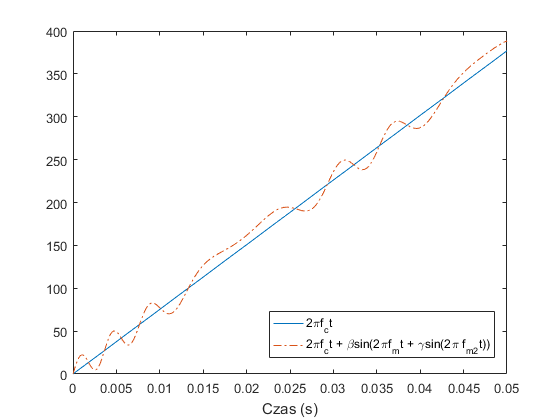
\includegraphics[width=10cm]{grafiki/fm_arg2}
	\captionsetup{justification=centering}
	\caption{Przebiegi czasowe argumentu funkcji sinus przed i po zagnieżdżonej modulacji FM.}
	\label{rys:fm_arg2}
\end{figure}
Linią ciągłą narysowano przebieg argumentu sygnału nośnego przed modulacją. Natomiast linia przerywana obrazuje przebieg argumentu sygnału po zagnieżdżonej modulacji częstotliwościowej. Na drodze eksperymentów można uzyskiwać w ten sposób naprawdę ciekawe brzmienia.
\subsection{Uzyskiwanie konkretnych brzmień}
W literaturze można znaleźć parametry syntezy FM, które pozwalają uzyskać brzmienie zbliżone do naturalnych dźwięków. W \cite{chowning} odnaleźć można na przykład parametry, za pomocą których można uzyskać brzmienie dzwona. Parametry te wyglądają następująco:

\begin{table}[h!]
\centering
	\begin{tabular}{ |c| c| }
	\hline
	Parametr & Wartość \\
	\hline
	$f_c$ & 200 Hz \\
	\hline
	$f_m$ & 280 Hz\\
	\hline
	$\beta$ & 10\\
	\hline
	
	\end{tabular}
\captionsetup{justification=centering}
\label{tab:fm_bell}
\caption{Parametry brzmienia dzwona.}
\end{table}
Jednak dźwięk samego zmodulowanego przebiegu nie ma charakteru brzmienia dzwona. Ważnym jest zastosowanie odpowiedniej obwiedni amplitudy uzyskanego przbiegu. W tym przypadku dobry wynik daje zastosowanie funkcji zanikającej ekspotencjalnie. Przykładem takiej funkcji jest wyrażenie:
\begin{equation} \label{equ:fm_belladsr}
A(t) = e^{-t}.
\end{equation}
Przebieg obwiedni opisanej za pomocą (\ref{equ:fm_belladsr}) pokazano na rysunku \ref{rys:fm_belladsr}.
\begin{figure}[H]
	\centering
	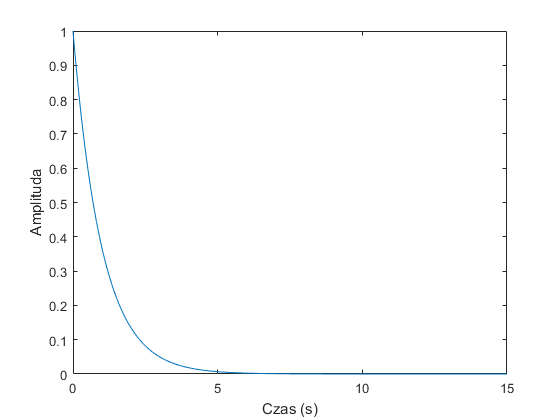
\includegraphics[width=10cm]{grafiki/fm_belladsr}
	\captionsetup{justification=centering}
	\caption{Kształt obwiedni w syntezie dźwięku dzwona.}
	\label{rys:fm_belladsr}
\end{figure}

\section{Implementacja syntezy FM}
W celu nie naruszania struktury pętli głównej programu wykonywanego na DSP, algortym syntezy dla metody FM został dostosowany do istniejącego kodu. Stąd generowanie dźwięku będzie realizowane w sposób blokowy. Blok ma rozmiar $N = 1024$ próbek. 
\subsection{Generowanie przebiegu}
W programie wykorzystywane są dwie tablice o $N$ próbkach, które naprzemiennie wysyłane są do przetwornika cyfrowo-analogowego. W czasie, gdy jedna z nich jest przetwarzana na sygnał analogowy, druga jest wypełniana nowymi próbkami przebiegu. W celu zachowania ciągłości pomiędzy blokami, wprowadzony został licznik bloków $k$, który odpowiada za odpowiednie przesuniecię w fazie generowanych sygnałów. Za generowanie pojedynczego tonu zmodulowanego częstotliwościowo odpowiada kod:
\begin{equation} \label{equ:fm_wzor2}
\text{waveform[i]} = \text{sinf}(2\pi f_c(i+kN)\frac{1}{F_s} + \beta \text{sinf}(2 \pi f_m(i+kN)\frac{1}{F_s}))
\end{equation}
\begin{tabular}{ l l l l}
	gdzie: & waveform &  - & tablica zmiennych typu float, \\
	&	$F_s$ & - & częstotliwość próbkowania,\\
	&	$i$ & - &  licznik iteracji, $i$ = 0, 1, 2, ..., N-1,\\
	&	$k$ & - &  licznik bloków.\\
\end{tabular} \\ \\
W (\ref{equ:fm_wzor2}) zastosowano funkcję "sinf" zamiast zwykłego "sin". Obie te funkcję należą do biblioteki math.h w języku C. Wybór "sinf" wynika z faktu, że funkcja "sin" operuje na zmiennych typu double (podwójna precyzja), a "sinf" na zmiennych typu float. Działania na zmiennych typu float są wykonywane szybciej. Kosztem jest mniejsza precyzja wykonywanych obliczeń.

Po wypełnieniu próbkami danej tablicy waveform, jest ona wysyłana do DAC. Licznik bloków jest modyfikowany w następujący sposób:
\begin{equation} \label{equ:fm_wzor3}
k \gets k + N - m.
\end{equation}
\begin{tabular}{ l l l l}
	gdzie: & $m$  &  - & liczba zakładkowanych próbek. \\
\end{tabular} \\ \\
Mechanizm zakładkowania, opisany w metodzie subtraktywnej, nie jest wyłączany przy aktywacji innych metod syntezy. Z tego powodu, licznik bloków jest pomniejszany o wartość $m$.
\subsection{Polifonia w syntezie FM}
Do generowania wielu tonów jednocześnie, wykorzystywana jest tablica wciśniętych klawiszy instrumentu, opisana w REALIZACJA->POLIFONIA. Jest ona przeglądana w pętli głównej programu i dla każdej częstotliwości, która się w niej znajduje, generowane jest $N$ próbek przebiegu w jednej z tablic "waveform". Generowanie pojedynczego bloku z uwzględnieniem polfionii opisuje wyrażenie:
\begin{equation} \label{equ:fm_wzor4}
\text{waveform[i]} =\left \{\begin{array}{ r l }
\text{sinf}(2\pi f_j(i+kN)\frac{1}{F_s} + \beta \text{sinf}(2 \pi f_m(i+kN)\frac{1}{F_s})), & \quad \text{dla } j = 0\\
\text{waveform[i]} + \text{sinf}(2\pi f_j(i+kN)\frac{1}{F_s} + \beta \text{sinf}(2 \pi f_m(i+kN)\frac{1}{F_s})), & \quad  \text{dla } j = 1, 2, ..., J-1
\end{array}
\right.
\end{equation}
\begin{tabular}{ l l l l}
	gdzie: & $J$ &  - & liczba wciśniętych klawiszy instrumentu, \\
		&	$i$ & - & licznik iteracji, $i$ = 0, 1, 2, ..., N-1,\\
		&	$f_j$ & - & częstotliwość j-tego tonu.\\
\end{tabular} \\ \\

Zastosowane rozwiązanie pozwala wygenerować do 6 tonów jednocześnie. 

\section{Interfejs użytkownika}
W projekcie autorskim, w przypadku syntezy FM, użytkownik może poprzez interfejs użytkownika określać parametry modulacji: amplitudę sygnału modulującego oraz jego częstotliwość.
\begin{figure}[H]
	\centering
	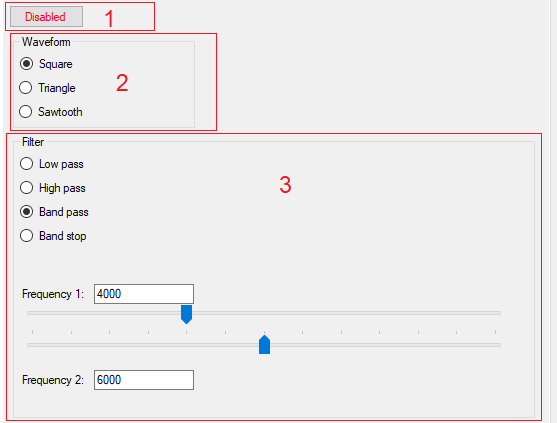
\includegraphics[width=12cm]{grafiki/sub_interface}
	\captionsetup{justification=centering}
	\caption{Interfejs użytkownika dla modulacji częstotliwościowej.}
	\label{rys:fm_interface}
\end{figure}
Na rysunku \ref{rys:fm_interface} zaznaczono dwie sekcje wykonanego interfejsu dla syntezy FM. W pierwszej z nich znajduje się przycisk, który służy do aktywacji tej metody syntezy dźwięku. Po naciśnięciu tego klawisza, DSP otrzymuje komunikat, po którym przechodzi w tryb syntezy FM.

W drugiej sekcji znajdują się suwaki pozwalające na wybór amplitudy oraz częstotliwości sygnału modulującego. Zmian tych wielkości można dokonywać na dwa sposoby:
\begin{itemize}
	\item za pomocą suwaków. W tym wypadku wartość ustawiona za pomocą suwaka zostanie automatycznie wpisana do pola tekstowego skojarzonego z tym suwakiem.
	\item Poprzez precyzyjne wpisanie wartości do pola tekstowego obok suwaka. W tej sytuacji suwak automatycznie się przesunie na pozycję odpowiadającą wpisanej wartości.
\end{itemize}
Zmianę parametrów należy zatwierdzić klawiszem "Set". Po jego naciśnięciu, odpowiednie komunikaty zostają przesłane do DSP.

%	\chapter{Badanie właściwości układu} 
Lorem ipsum dolor sit amet, consectetur adipiscing elit, sed do eiusmod tempor incididunt ut labore et dolore magna aliqua. Ut enim ad minim veniam, quis nostrud exercitation ullamco laboris nisi ut aliquip ex ea commodo consequat. Duis aute irure dolor in reprehenderit in voluptate velit esse cillum dolore eu fugiat nulla pariatur. Excepteur sint occaecat cupidatat non proident, sunt in culpa qui officia deserunt mollit anim id est laborum.

\section{Przewidywana transmitancja}
Lorem ipsum dolor sit amet, consectetur adipiscing elit, sed do eiusmod tempor incididunt ut labore et dolore magna aliqua. Ut enim ad minim veniam, quis nostrud exercitation ullamco laboris nisi ut aliquip ex ea commodo consequat. Duis aute irure dolor in reprehenderit in voluptate velit esse cillum dolore eu fugiat nulla pariatur. Excepteur sint occaecat cupidatat non proident, sunt in culpa qui officia deserunt mollit anim id est laborum.
\begin{table}[H]
	\caption{Porównanie położenia biegunów modelu teoretycznego i zidentyfikowanego.}
	\label{bieguny_porownanie}
	\centering
	\begin{tabular}{|c|c|c|}
		\hline 
		Biegun & Model teoretyczny & Model zidentyfikowany 	\\
		\hline
	$\lambda_{0}$							& $0$ 				& $0$ 				\\	\hline
 	$\lambda_{1}$							& $5,940$			& $5,785$			\\	\hline
	$\lambda_{2}$							& $-6,648$			& $-7,076$			\\	\hline
	$\lambda_{3}$ 							& $-1,131$			& $-1,872$			\\ 	\hline
	\end{tabular} 
\end{table}

	\chapter{Modelowanie fizyczne}
W odniesieniu do syntezy dźwięku, modelowanie fizyczne polega na opisaniu zależności fizycznych występujących w trakcie gry na danym instrumencie. Niektóre z nich skupiają się na własnościach materiałowych, inne opisują interakcję fizyczną instrumentalisty z instrumentem. Generowanie fali dźwiękowej za pomocą takiego modelu opiera się na wykorzystaniu równań matematycznych oraz odpowiednich algorytmów pozwalających na scalenie wszystkich wykorzystywanych w danym momencie metod. Istnieją różne postacie opisów modeli fizycznych instrumentów:
\begin{itemize}
	\item równania różniczkowe,
	\item synteza falowodowa,
	\item modelowanie reakcji masy,
	\item przestrzeń stanów,
	\item transmitancja.
\end{itemize}

W niniejszym rozdziale opisano działanie syntezy falowodowej, która miała bardzo duże znaczenie w rozwoju modelowania fizycznego instrumentów. Jest to zarazem jedyna z metod modelowania fizycznego, która jest implementowana w urządzeniach komercyjnych, takich producentów jak Yamaha czy Korg. W kolejnych podrozdziałach przedstawiono syntezę dźwięku skrzypiec oraz fletu na podstawie schematów falowodowych. Opisano również implementację tej metody na procesorze DSP.


\section{Synteza falowodowa}
W instrumentach muzycznych proces generowania dźwięku opiera się na pojęciu fal bieżących wewnątrz drgających obiektów. Wykorzystując ich fizyczny opis, można zasymulować ich działanie za pomocą odpowiedniego algorytmu. Na tej zasadzie działa metoda cyfrowych falowodów (ang. digital waveguide). Pozwala ona na symulowanie  rozchodzenia się fal bieżących w~elementach instrumentów takich jak struna gitary czy tuba instrumentu dętego. Metoda ta została zaproponowana przez Juliusa O. Smitha z Uniwersytetu Stanforda w latach 90. Od tego czasu służy do syntezy brzmień takich instrumentów jak gitary, instrumenty smyczkowe czy instrumenty dęte.

%\section{Linia opóźniająca}
Do opisu cyfrowego falowodu potrzebna jest znajmość pojęcia linii opóźniającej (ang. delay line). Jest to element wprowadzający opóźnienie czasowe pomiędzy próbkami, które do niego wchodzą, a próbkami, które z niego wychodzą. 
\begin{figure}[H]
	\centering
	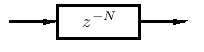
\includegraphics[width=5cm]{grafiki/linia}
	\captionsetup{justification=centering}
	\caption{Linia opóźniająca o długości N.}
	\label{rys:delay_line}
\end{figure}
Na rysunku \ref{rys:delay_line} zobrazowana została linia opóźniająca o długości $N$ próbek. Można ją przedstawić także jako $N$ bloków o jednostkowym opóźnieniu połączonych szeregowo (patrz rysunek \ref{rys:model_delay_line2}).
\begin{figure}[H]
	\centering
	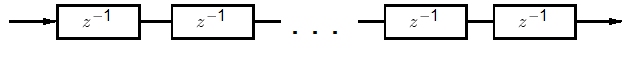
\includegraphics[width=10cm]{grafiki/model_linie}
	\captionsetup{justification=centering}
	\caption{N bloków o jednostkowym opóżnieniu.}
	\label{rys:model_delay_line2}
\end{figure}
 Implementacja linii opóźniającej sprowadza się do wykorzystania tablicy o $N$ elementach oraz zmiennych wskaźników do pierwszego i ostatniego z jej elementów. Dzięki temu, opóźnianie danych w tablicy odbywa się bez konieczności przepisywania jej całej zawartości w każdej chwili czasu. W celu uzyskania opóźnień czasowych o niecałkowitą liczbę próbek, stosuje się prostą interpolację liniową pomiędzy dwoma sąsiednimi danymi.

%\section{Cyfrowy falowód}
% https://edu.pjwstk.edu.pl/wyklady/mul/scb/main37.html

Cyfrowy falowód to w uproszczeniu dwukierunkowa linia opóźniająca. Implementuje się go zatem jako dwie linie opóźniające, w których fale rozchodzą się w przeciwnych kierunkach. Linie te są ze sobą sprzężone na końcach za pomocą inwerterów. Cyfrowy falowód można interpretować na przykład jako strunę - dłuższa struna będzie wiązała się z dłuższym falowodem. Oznacza to, że można określić prędkość odchylania się struny w dowolnym punkcie jej długości. Dokonuje się tego poprzez sumowanie, w danym punkcie struny, prędkości fali rozchodzącej się w jednym kierunku oraz predkości fali rozchodzącej się w drugim kierunku.
\begin{figure}[H]
	\centering
	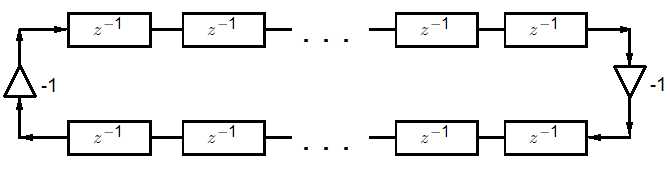
\includegraphics[width=10cm]{grafiki/model_falowod}
	\captionsetup{justification=centering}
	\caption{Cyfrowy falowód jako złożenie dwóch linii opóźniających.}
	\label{rys:model_falowod}
\end{figure}
\section{Synteza dźwięku skrzypiec}
Instrumenty smyczkowe są jedną z grup instrumentów, które modeluje się za pomocą cyfrowych falowodów. W niniejszym podrozdziale przedstawiona zostanie zasada działania syntezy dźwięku skrzypiec z wykorzystaniem właśnie tej metody, implementacja zastosowana w autorskim projekcie oraz uzyskane wyniki.

\subsection{Zasada działania syntezy dźwięku skrzypiec}
Syntezę dźwięku skrzypiec można podzielić na trzy zakresy:
\begin{itemize}
	\setlength\itemsep{-3pt}
	\item symulację interakcji pomiędzy smyczkiem a struną,
	\item symulację rozchodzenia się fal w strunie,
	\item symulację przechodzenia fal ze strun do korpusu skrzypiec poprzez mostek.
\end{itemize}
Kompletny schemat blokowy modelu realizującego syntezę dźwięku instrumentu smyczkowego został pokazany na rysunku \ref{rys:schematblokowy} pochodzącym z \cite{bowed_3}.
\begin{figure}[H]
	\centering
	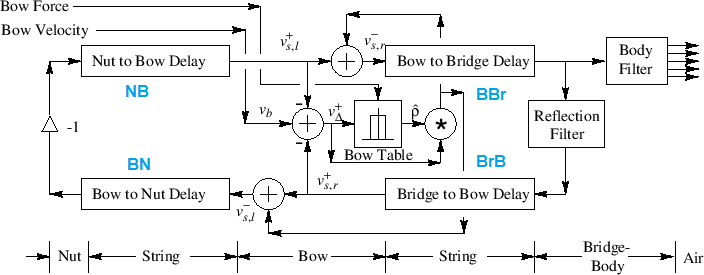
\includegraphics[width=12cm]{grafiki/schematblokowy}
	\captionsetup{justification=centering}
	\caption{Schemat blokowy modelu realizującego syntezę dźwięku \cite{bowed_3}.}
	\label{rys:schematblokowy}
\end{figure}
Poszczególne elementy skrzypiec zostały oznaczone na rysunku \ref{rys:skrzypce}.
\begin{figure}[H]
	\centering
	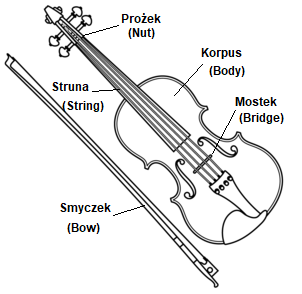
\includegraphics[width=5cm]{grafiki/skrzypce}
	\captionsetup{justification=centering}
	\caption{Elementy skrzypiec istotne dla symulacji.}
	\label{rys:skrzypce}
\end{figure}

W następnych podrozdziałach omówione zostaną kolejne obszary syntezy w oparciu o \cite{bowed_smith}. Należy mieć na uwadzę, że ostatecznie synteza tego typu przeprowadzana jest na DSP w czasie rzeczywistym.


\subsubsection{Rozchodzenie się fal w strunie}
Rozchodzenie się fal w strunie jest symulowane z wykorzystaniem cyfrowego falowodu oraz filtrów, które mają za zadanie odwzorować odbijanie się fal na jej końcach. Fale rozchodzące się w~strunie wpływają na prędkość jej lokalnych odchyleń. Ta prędkość wraz z prędkością przesuwania się smyczka po strunie stanowią podstawę do syntezy dźwięku skrzypiec. 


%\subsubsection{Odbicia na końcach struny}
Fale w strunie rozchodzą się w obu kierunkach, aż dotrą do końca struny - mostka, prożka lub palca skrzypka. Elementy te, oznaczone na rysunku \ref{rys:skrzypce}, uniemożliwiają strunie ruch, zatem fale się od nich odbijają. Fala, która dociera do jednego z tych elementów, zostaje częściowo odbita, więc zmienia się jej kierunek rozchodzenia. Odbijanie implementowane jest jako przepisywanie danej próbki z końca jednej linii opóźniającej do początku drugiej w obrębie jednego cyfrowego falowodu. Przy takim odbiciu następuje zmiana znaku próbki.
Dodatkowo, aby uwzględnić straty zależne od częstotliwości zachodzące przy odbiciach oraz samym rozchodzeniu się fali, co najmniej jedno odbicie modeluje się za pomocą filtra dolnoprzepustowego o wzmocnieniu mniejszym od 1. 
Ponadto do modelowania zjawiska dyspersji można użyć filtra wszechprzepustowego \cite{allpass}.


\subsubsection{Interakcja pomiędzy smyczkiem a struną}
Smyczek przesuwany po strunie, na skutek tarcia pomiędzy jego włosiem a struną, wprawia ją w ruch. Dopóki siła tarcia jest większa niż siła sprężystości struny, to struna odchyla się zgodnie z~ruchem smyczka. Jednak w momencie kiedy siła sprężystości będzie odpowiednio duża, struna przestanie podążać za smyczkiem i wykona gwałtowny ruch w kierunku przeciwnym do przesuwania smyczka.  Cykl ten powtarza się przez cały czas trwania pojedynczego jednokierunkowego ruchu smyczka po strunie.  \\
Do modelowania tego zjawiska wykorzystuje się współczynnik odbicia $\rho$, który powstał na podstawie opisu tarcia pomiędzy struną a smyczkiem \cite{bowed_3}. Jego wykres przedstawiono na rysunku \ref{rys:tarcie}. Przy wartości współczynnika odbicia $\rho$ równej $1$, struna podąża za smyczkiem. Im wartość $\rho$ jest mniejsza, tym większy jest poślizg struny.
\begin{figure}[H]
	\centering
	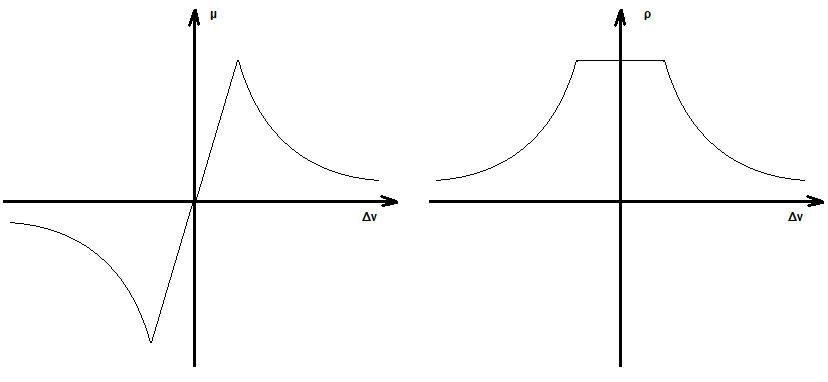
\includegraphics[width=8cm]{grafiki/tarcie2}
	\captionsetup{justification=centering}
	\caption{Współczynnik odbicia $\rho(\Delta v)$.}
	\label{rys:tarcie}
\end{figure}
Wartości współczynnika odbicia $\rho$ są wyliczane raz, według wzoru
\begin{equation} \label{equ:model_wsp_odbicia}
\rho(\Delta v) = \left \{\begin{array}{ r l }
0.98, & \quad \text{dla } (|3 (\Delta v + 0.001) | + 0.75)^{-4} > 0.98\\
0.01, & \quad  \text{dla } (|3 (\Delta v + 0.001) | + 0.75)^{-4} < 0.01\\
(|3 (\Delta v + 0.001) | + 0.75)^{-4}, & \quad \text{w pozostałych przypadkach.}
\end{array}
\right.
\end{equation}
\begin{tabular}{ l l l l}
	gdzie: & $\Delta v$ &  - & różnica prędkości pomiędzy smyczkiem a struną.
\end{tabular} \\ \\
i przechowywane w tablicy. Następnie wyznacza się różnicę pomiędzy prędkościami struny oraz smyczka $v_{diff}$:
\begin{equation} \label{equ:wzor1}
v_{diff}[t] = v_b[t] - v_{l}^{+} - v_{r}^{+}
\end{equation}
\begin{tabular}{ l l l l}
	gdzie: & $t$ &  - & obecna chwila czasu, \\
	&	$v_b$ & - &  prędkość smyczka, \\
	&	$v_{l}^{+}$ & - & prędkość struny przychodząca wraz z falą z lewej strony,\\
	&	$v_{r}^{+}$ & - &  prędkość struny przychodząca wraz z falą z prawej strony.\\
\end{tabular} \\ \\
Dalej wyznaczone zostają prędkości struny, które rozejdą się od smyczka odpowiednio w lewą i prawą stronę:
\begin{equation} \label{equ:wzor2}
v_{l}^{-} = v_r^{+} +  \rho(v_{diff}[t])v_{diff}[t]
\end{equation}
\begin{equation} \label{equ:wzor3}
v_{r}^{-} = v_l^{+} +  \rho(v_{diff}[t])v_{diff}[t]
\end{equation}
\begin{tabular}{ l l l l}
	gdzie: & $\rho(v)$ &  - & stablicowana funkcja przedstawiona na rysunku \ref{rys:tarcie}. \\
	
\end{tabular}
\vspace{6pt}

W wyniku pobudzania smyczkiem, struna wpada w charakterystyczny ruch, który jest nazywany ruchem Helmholtza. Jak pokazano w \cite{bowed_2}, próbkowanie prędkości wychyleń struny - będącej w~ruchu Helmholtza - w danym punkcie jej długości, daje sygnał zbliżony do przebiegu piłokształtnego. Zgadza się to z wcześniej opisanym zjawiskiem cyklicznego podążania struny za smyczkiem oraz ślizgania się po nim.

\subsubsection{Przechodzenie fal ze strun do korpusu skrzypiec}\label{sec:model_violinarma}

Ostatnim etapem jest przenoszenie się fal akustycznych ze strun do korpusu skrzypiec, które zachodzi w mostku. Później drgający korpus wprowadza te fale do powietrza i tak powstaje słyszalny dźwięk. W tym celu bada się funkcję przenoszenia pomiędzy mostkiem a powietrzem. 

W \cite{bowed_smith} do zbadania transmitancji mostek-korpus, zaproponowano metodę, w której sygnałem wyjściowym jest dźwięk w powietrzu, a sygnałem wejściowym jest siła działająca na mostek. Przyjęcie siły jako sygnału na wejściu tego układu wynika z tego, że mostek jest nieruchomym mocowaniem struny. Zatem prędkość mostka jest znikoma. Na mostek unieruchamiający wibrującą strunę działa siła wynikająca z prędkości odchyleń tej struny. W przytoczonej pracy, do pomiaru dźwięku został wykorzystany mikrofon, umieszczony w odległości około 30cm (jedna stopa) od czoła instrumentu, oraz przetwornik piezoelektryczny, przyklejony żywicą epoksydową do mostka, co pokazano na rysunku \ref{rys:pomiary}. Aby uzyskać jak najlepszy stosunek sygnału do szumu sygnału wyjściowego, mikrofon nie mógł znajdować się zbyt daleko oraz same pomiary powinny być przeprowadzane w komorze bezechowej.

\begin{figure}[H]
	\centering
	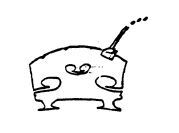
\includegraphics[width=5cm]{grafiki/pomiary}
	\captionsetup{justification=centering}
	\caption{Przetwornik piezoelektryczny przyklejony do mostka skrzypiec \cite{bowed_smith}.}
	\label{rys:pomiary}
\end{figure}

Autor \cite{bowed_smith} dokonał prób z rozmaitymi sposobami pobudzania struny: prostego smyczkowania, techniki glissando, ze strunami owiniętymi tkaniną (próbowano uchwycić szum, syczenie smyczka lekko przesuwanego po strunie w pobliżu mostka), uderzania przetwornika śrubokrętem oraz szarpania strun kostką gitarową w pobliżu mostka. Najlepsze wyniki otrzymano ostatnim sposobem.

Uzyskane w ten sposób widmo częstotliwościowe poddano odpowiedniej obróbce. Między innymi zmniejszono częstotliwość próbkowania oraz wygładzono przebieg widma. Następnie próbowano dopasować do niego proces autoregresyjny używając różnych metod identyfikacji. Najlepszy wynik uzyskano stosując normę Hankela, a końcowe dopasowanie uzyskanych charakterystyk pokazano na rysunku \ref{rys:hankel}.

\begin{figure}[H]
	\centering
	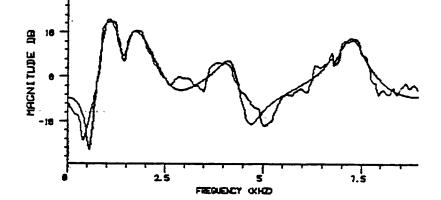
\includegraphics[width=8cm]{grafiki/hankel}
	\captionsetup{justification=centering}
	\caption{Dopasowanie widma amplitudowego procesu AR do pomierzonego \cite{bowed_smith}.}
	\label{rys:hankel}
\end{figure}

Autorzy \cite{bowed_4} przeprowadzili podobne pomiary, z tym, że strunę pobudzali młotkiem wyposażonym w piezoelektryczny miernik siły, a mikrofon umieścili metr od instrumentu.

W \cite{bowed_2} pomiarów dokonano nieco inaczej. W opisanej tam metodzie, wykorzystany został młotek wyposażony w czujnik siły. Młotkiem tym uderzano w mostek w kierunku prostopadłym do strun. Na mostku z kolei, zamontowany był akcelerometr mierzący przyspieszenie również w~kierunku prostopadłym do strun.

Wszystkie te działania zmierzały do zidentyfikowania modelu autoregresyjnego, który odwzorowuje szczyty rezonansowe pomierzonego widma częstotliwościowego. Model ten jest pobudzany sygnałem uzyskanym z próbkowania prędkości struny. Uzyskany w ten sposób sygnał wyjściowy to model dźwięku skrzypiec.

\subsection{Implementacja syntezy dźwięku skrzypiec}
Schemat z rysunku \ref{rys:schematblokowy} na potrzeby implementacji można nieco uprościć. Przekształcając schemat, dwie linie opóźniające (BN i NB) rozdzielone jedynie inwerterem można połączyć w~jedną (DL1), której znak jest zmieniany na końcu. Tak samo można zrobić z dwoma liniami opóźniającymi rozdzielonymi filtrem dolnoprzepustowym (BBr i BrB). Takie działania nie mają wpływu na efekt końcowy syntezy, a dzięki nim zaimplementować trzeba tylko dwie linie opóźniające, zamiast czterech. Ponadto można zrezygnować z elementu modelu związanego z wpływem siły nacisku smyczka na strunę. Uproszczony schemat blokowy został pokazany na rysunku \ref{rys:model_violin_schemat}.
\begin{figure}[H]
	\centering
	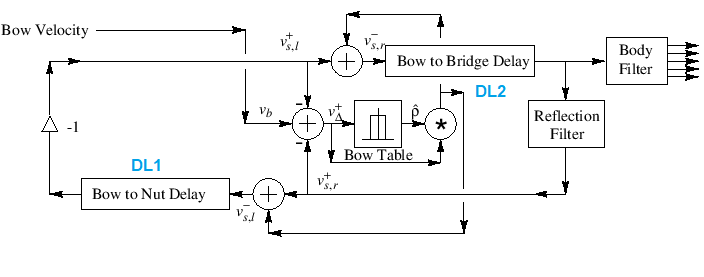
\includegraphics[width=12cm]{grafiki/model_violin_schemat}
	\captionsetup{justification=centering}
	\caption{Uproszczony schemat blokowy syntezy falowodowej skrzypiec [].}
	\label{rys:model_violin_schemat}
\end{figure}
Dzięki takiej redukcji bloków funkcjonalnych, zaimplementować należy tylko dwie linie opóźniające: bridgeDelay[.] i neckDelay[.]. Długość pojedynczej linii (liczba elementów tablicy) zależy od częstotliwości najniższego z generowanych tonów i jest całkowitą częścią wielkości opisanej wzorem:
\begin{equation} \label{equ:model_ndelays}
L_{DL} = \frac{F_s}{F_{lowest}}
\end{equation}
\begin{tabular}{ l l l l}
	gdzie: & $F_{lowest}$ &  - & najniższa generowana częstotliwość. \\
\end{tabular}\\
Z linią opóźniającą skojarzone są zmienne przechowujące indeksy początkowe i końcowe linii: całkowite inPoint i outPoint oraz zmiennoprzecinkowy outPointer. 
\begin{figure}[H]
	\centering
	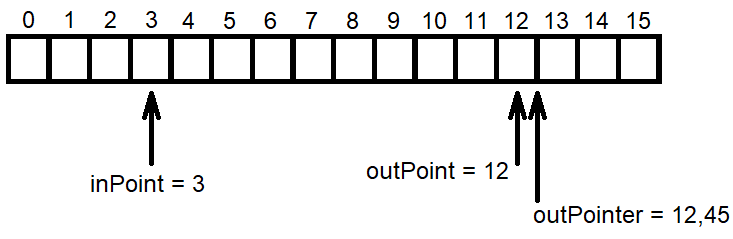
\includegraphics[width=10cm]{grafiki/model_violin_wskazniki}
	\captionsetup{justification=centering}
	\caption{Schemat linii opóźniającej i jej wskaźników.}
	\label{rys:model_violin_wskazniki}
\end{figure}
Na rysunku \ref{rys:model_violin_wskazniki} przedstawiono schemat linii opóźniającej i opisane wskaźniki. W każdej chwili czasu wskaźniki te są inkrementowane (przykład dla neckDelay[.]):
\begin{equation} \label{equ:model_wskazniki}
\text{neck\_inPoint} \gets \left \{ 
\begin{array}{ l l}
\text{neck\_inPoint+1} &  \text{gdy neck\_inPoint}+1 < L_{DL} \\
0 &  \text{gdy neck\_inPoint}+1 \geqslant L_{DL}
\end{array},
\right.
\end{equation}
\begin{equation} \label{equ:model_wskazniki2}
\text{neck\_outPoint} \gets \left \{ 
\begin{array}{ l l}
\text{neck\_outPoint+1} &  \text{gdy neck\_outPoint}+1 < L_{DL} \\
0 &  \text{gdy neck\_outPoint}+1 \geqslant L_{DL}
\end{array}.
\right.
\end{equation}
 Do komórki o indeksie inPoint wpisywana jest nowa próbka, a w komórce o indeksie outPoint zapisana jest próbka "wyjściowa". Prawdziwe wyjście linii opóźniających najczęściej nie ma całkowitego indeksu, zatem obliczane jest jako średnia ważona pomiędzy dwoma sąsiednimi próbkami. W tym celu obliczyć należy współczynnik wagowy
 \begin{equation} \label{equ:model_alpha}
\alpha_{neck} = \text{neck\_outPointer} - \text{neck\_outPoint},
 \end{equation}
który służy do wyznaczania wyjścia jako
 \begin{equation} \label{equ:model_neckoutput}
\text{neck\_output} = (1 - \alpha_{neck}) \text{neckDelay[neck\_outPoint]} + \alpha_{neck} \text{neckDelay[neck\_nextOut]}
\end{equation}
\begin{tabular}{ l l l l}
	gdzie: & neck\_nextOut & - & przyjmuje wartość: neck\_outPoint+1 lub 0. \\
\end{tabular} \\
Na końcu jednej z linii (bridgeDelay[.]) znajduje się prosty filtr dolnoprzepustowy (stringFilter). Każda wychodząca próbka poddawana jest filtracji według wzoru:
 \begin{equation} \label{equ:model_stringfilter}
\text{stringFilter[n]} = \text{SF}\_\text{g}*\text{SF}\_\text{b}*\text{bridge\_output} - \text{SF}\_\text{a}* \text{stringFilter[n-1]}.
\end{equation}
\begin{tabular}{ l l l l}
	gdzie: & \text{SF}\_\text{g} & - & wzmocnienie filtra równe 0.95, \\
			& \text{SF}\_\text{a} & - & współczynnik a filtra równy $\frac{24000}{5F_s} - 0.55$, \\
			& \text{SF}\_\text{b} & - & współczynnik b filtra równy $1+\text{SF}\_\text{a}$. \\
\end{tabular} \\
Następnie oblicza się sumę wyjść stringFilter i neck\_Output (wyjścia te dodatkowo zmieniają znak na przeciwny). Uzyskany rezultat dodawany jest do zmiennej opisującej prędkość smyczka pomnożonej przez ADSR:
 \begin{equation} \label{equ:model_deltav}
\Delta v = \text{ADSR[n]} v_b + (\text{stringFilter[n]} + \text{neck\_output})
\end{equation}
\begin{tabular}{ l l l l}
	gdzie: & $v_b$ &  - & to maksymalna prędkość smyczka osiągana w symulacji, \\
	& ADSR[n] &  - & wartość obwiedni w danej chwili czasu. \\
\end{tabular} \\
Na podstawie wartości $\Delta v$ oblicza się nową prędkość struny:
 \begin{equation} \label{equ:model_newv}
v_{new} = \rho (\Delta v) \Delta v
\end{equation}
\begin{tabular}{ l l l l}
	gdzie: & $\rho (\Delta v)$ &  - & wyznacza się korzystając z wzoru (\ref{equ:model_wsp_odbicia}). \\
\end{tabular} \\
Nowa wartość prędkości jest wprowadzana do linii opóźniających wraz z wartościami odbić:
 \begin{equation} \label{equ:model_newv2}
\text{neckDelay[neck\_inPoint]} = v_{new} - \text{stringFilter[n]},
\end{equation}
 \begin{equation} \label{equ:model_newv3}
\text{bridgeDelay[neck\_inPoint]} = v_{new} - \text{neck\_output}.
\end{equation}

Ostatnim krokiem jest filtracja wyjściowych próbek bridge\_output za pomocą procesu ARMA opisanego w części \ref{sec:model_violinarma}.
W celu uzyskania efektu Vibrato, należy w każdej chwili czasu modyfikować zmienną neck\_outPointer w rytm sygnału sinusoidalnego o niewielkiej częstotliwości. Modyfikacja ta pociąga za sobą konieczność aktualizowania współczynnika wagowego $\alpha _{neck}$ oraz wskaźnika neck\_outPoint. 
%\chapter{Implementacja syntezy dźwięku skrzypiec}
%\section{Implementacja syntezy dźwięku skrzypiec}
%\subsection{Implementacja syntezy dźwięku skrzypiec}
%\subsubsection{Implementacja syntezy dźwięku skrzypiec}
\subsection{Wyniki eksperymentalne}
Opisana implementacja pozwala wygenerować dźwięk o charakterze instrumentu smyczkowego. Na końcowe wrażenia słuchowe, poza samą syntezą falowodową, duży wpływ mają dodatkowe efekty akustyczne takie jak: odpowiednie kształtowanie obwiedni czy odpowiednio dobrany efekt Vibrato (częstotliwość, amplituda). Wyniki symulacji przeprowadzonej w środowisku Matlab przedstawiono na rysunku \ref{rys:model_violin_matlab}.
\begin{figure}[H]
	\centering
	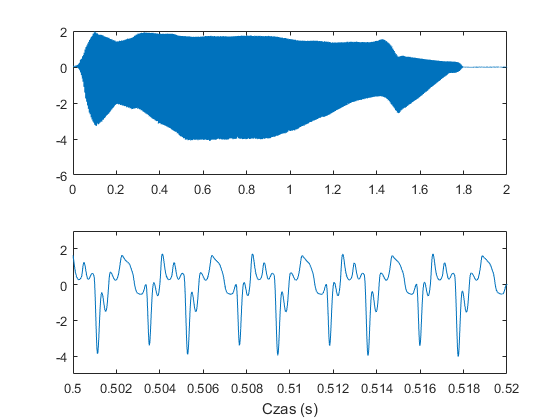
\includegraphics[width=12cm]{grafiki/model_violin_matlab}
	\captionsetup{justification=centering}
	\caption{Wygenerowany dźwięk skrzypiec. Ton o częstotliwości 240 Hz.}
	\label{rys:model_violin_matlab}
\end{figure}

	\section{Synteza dźwięku fletu}

W literaturze można znaleźć wiele różnych metod syntezy dźwięku instrumentów dętych drewnianych. Ich modele są przedstawione zazwyczaj za pomocą różniczkowych równań fizycznych lub w postaci falowodów cyfrowych. 
%klarnet: https://www.researchgate.net/publication/4333455_Representation_of_solo_clarinet_music_by_physical_modeling_synthesis
%gestures: https://www.researchgate.net/publication/5323798_Gesture_synthesis_basic_control_of_a_flute_physical_model
%slide-flute perry cook: https://quod.lib.umich.edu/cache//b/b/p/bbp2372.1992.072/bbp2372.1992.072.pdf#page=1;zoom=75
Przykładem takiej pracy naukowej jest artykuł na temat modelu fizycznego klarnetu, w którym autorzy opisują równaniami różniczkowymi interakcje poszczególnych elementów instrumentu dętego drewnianego \cite{flute_klarnet}. Inna praca naukowa porusza temat kontroli modelu fletu, w którym autorzy skupili się na opisaniu zależności fizycznych związanych głównie z grą flecisty \cite{flute_flecista}, takich jak: ciśnienie w ustach instumentalisty, odległość od fletu oraz szerokość otwarcia ust. Kolejnym przykładem artykułu opisującego model instrumentu dętego drewnianego jest praca P. Cooka przedstawiająca falowody cyfrowe fletu suwakowego (ang. slide flute) oraz klarnetu \cite{flute_cook}.

%o tym ze trudno jest zrobić wielootworowe --> ta ksiazka computer music costam


W niniejszym podrozdziale przedstawiono dwa podejścia do implementacji syntezy dźwięku drewnianego instrumentu dętego:
\begin{itemize}
	\setlength\itemsep{-3pt}
	\item za pomocą falowodu cyfrowego,
	\item za pomocą zidentyfikowanego modelu ARMA.
\end{itemize}
Na końcu podrozdziału przedstawiono porównanie wyników obu tych podejść do syntezy, na podstawie wygenerowanych dźwięków.

\subsection{Synteza falowodowa instrumentów dętych}
%https://ccrma.stanford.edu/~jos/pasp/Digital_Waveguide_Models.html
%https://quod.lib.umich.edu/cache//b/b/p/bbp2372.1992.072/bbp2372.1992.072.pdf#page=1;zoom=75

Synteza falowodowa instrumentów dętych drewnianych opiera się głównie na cyfrowych liniach opóźniających, które symulują odbicia fali w komorze dźwiękowej (ang. bore) tego rodzaju instrumentów. Komorę dźwiękową można uprościć do cylindra, w którym rozchodzi się fala. Jest to znaczna zaleta metody falowodowej, gdyż dowolny element instrumentu dętego może zostać zamodelowany za pomocą zestawu tub cylindrycznych.

\begin{equation} \label{equ:flute_row_falowe}
\frac{\partial^2 p}{\partial t^2} = c^{2}\frac{\partial^2 p}{\partial x^2}
\end{equation}
\begin{tabular}{ l l l l}
	gdzie: 	&	$p$ & - &  ciśnienie, \\
	&	$x$ & - &  długość korpusu instrumentu dętego,\\
	&	$c$ & - &  prędkość propagacji dźwięku w powietrzu,\\
	&	$t$ & - &  czas. \\
\end{tabular} \\

%https://sound.eti.pg.gda.pl/student/eim/synteza/macmal/
Jednowymiarowe równanie falowe (\ref{equ:flute_row_falowe}) przedstawia rozchodzenie się fali płaskiej w nieskończenie długim cylindrze. Rozwiązaniem równania jest superpozycja dwóch fal ciśnienia (fal dźwiękowych) rozchodzących się w przeciwnych kierunkach komory dźwiękowej instrumentu dętego.


\subsubsection{Model}
W niniejszej pracy, syntezę falowodową dźwięku instrumentu dętego drewnianego oparto o schemat blokowy przedstawiony przez P. Cooka w 1992 roku.

\begin{figure}[H]
	\centering
	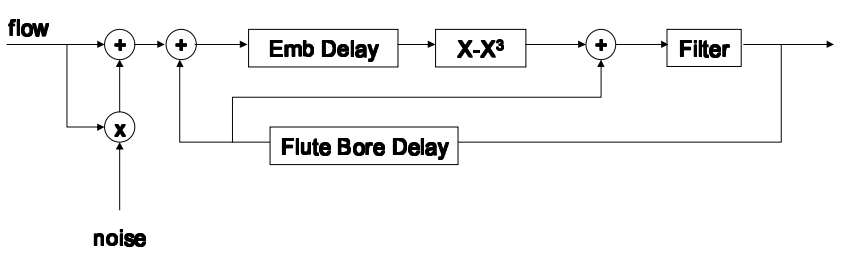
\includegraphics[width=14cm]{grafiki/flute_waveguide_mod}
	\captionsetup{justification=centering}
	\caption{Model falowodowy prostego instrumentu dętego drewnianego.}
	\label{rys:flute_cook}
\end{figure}

%https://courses.cs.washington.edu/courses/cse467/05wi/pdfs/lectures/15-waveguideInstruments.pdf
Wejściem systemu przedstawionego na rysunku \ref{rys:flute_cook} jest przepływ powietrza. Szum zostaje dodany w celu zasymulowania odgłosu wydechu flecisty. 
Interakcja między ustnikiem a komorą dźwiękową fletu przedstawiona została równaniem matematycznym $x-x^3$. Końcówka komory dźwiękowej odbija niskie częstotliwości - ta część została zasymulowana poprzez dodanie filtra dolnoprzepustowego przed wyjściem sygnału. Elementy "Emb Delay" oraz "Flute Bore Delay" to linie opóźniające, odpowiadające opóźnieniom fali w ustniku oraz w komorze dźwiękowej fletu. 
Obliczenie jednej próbki syntezowanego dźwieku na podstawie rysunku \ref{rys:flute_cook} wymaga 9 mnożeń oraz 6 operacji sumowania.

\subsubsection{Implementacja}
Implementację syntezy falowodowej w autorskim programie realizowanym na procesorze DSP,  wzorowano również na schemacie \ref{rys:flute_cook}. Przepływ powietrza (\emph{flow}) został zaimplementowany jako fala sinusoidalna o odpowiedniej obwiedni \cite{flute_prezka}. Szum dochodzący do utworzonego sygnału został zasymulowany funkcją rand(), a jego amplituda została przeskalowana. Sygnały sinusoidy i szumu są sumowane, a następnie trafiają do pętli zamkniętej, którą zaimplementowano w postaci pętli "for". Charakter brzmienia takiego modelu fletu zmienia się w zależności od parametrów wzmocnienia obu linii sprzężenia zwrotnego oraz wartości opóźnień "Emb Delay" i "Flute Bore Delay".

Jeden blok danych na procesorze DSP zawiera 1024 próbek. Linie opóźniające przesuwają próbki o kilkadziesiąt indeksów w tył. Oznacza to, iż pierwsza próbka nowego bloku danych, musi sięgnąć do poprzednio wygenerowanej tablicy. Do implementacji wykorzystano mechanizm tablicowy typu "ping-pong". Po wygenerowaniu pełnego bloku danych, pierwsza tablica przepisuje wszystkie wartości do drugiej. Następnie pierwsza tablica zostaje wyzerowana. Opóźnione próbki, do których należy się odnieść przy generowaniu nowego bloku danych, znajdują się w drugiej tablicy. Takim mechanizmem zapewniono ciągłość generowanego sygnału, bez błędów obliczeniowych.

\subsection{Synteza na podstawie modelu ARMA}
W tym punkcie przedstawiono identyfikację modelu matematycznego fletu, na podstawie którego przeprowadzono później syntezę dźwięku. Do rozpoznania modelu instrumentu użyto tonu "A" razkreślnego o częstotliwości 440 Hz. Dźwięk wygenerowany przez grę na flecie zmienia swoją charakterystykę w czasie. Oznacza to, iż jego model również zmienia się w trakcie nagranego przebiegu sygnału. Do identyfikacji wybrano te część nagrania, w której model instrumentu jest w stanie ustalonym.

\subsubsection{Identyfikacja modelu}
Identyfikacja modelu matematycznego instrumentu została przeprowadzona poprzez manualne dopasowanie zer i biegunów modelu do widma nagrania.
Proces identyfikacji przeprowadzono w środowisku symulacyjnym Matlab. Na nagranym fragmencie sygnału przeprowadzono dyskretną transformację Fouriera za pomocą algorytmu FFT.

Identyfikacja procesu modelem wysokiego rzędu za pomocą funkcji wbudowanych w środowisku Matlab dawała lepsze rezultaty niż manualne szukanie pików i dolin. Taki sposób nie pozwalał jednak na późniejszą parametryzację modelu dla różnej wysokości dźwięków. Z tego powodu, autorzy zrezygnowali w automatycznej identyfikacji modelu ARMA.

% WYKRESSSSS
\begin{figure}[H]
	\centering
	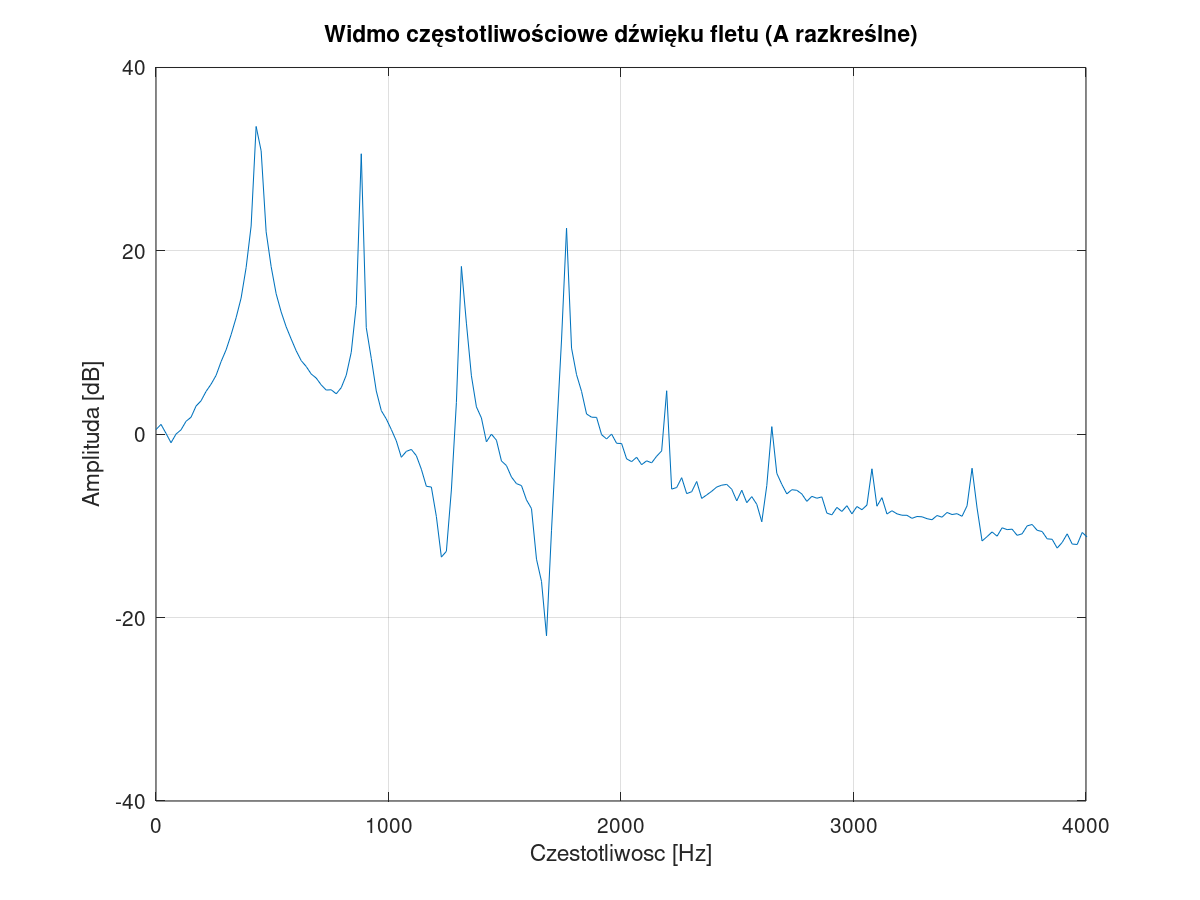
\includegraphics[width=12cm]{grafiki/flute_spectrum_orig}
	\captionsetup{justification=centering}
	\caption{Charakterystyka amplitudowa nagranego sygnału fletu.}
	\label{rys:flute_spectrum}
\end{figure}
% WYKRESSSS

Na rysunku \ref{rys:flute_spectrum} można zauważyć wyraźne piki oraz doliny charakterystyki częstotliwościowej nagranego sygnału. Siedem pierwszych pików charakterystyki zostało zinterpretowanych jako bieguny modelu, natomiast sześć pierwszych dolin zostały potraktowane jako jego zera. Liczba wybranych pików i dolin wziętych pod uwagę przy tworzeniu modelu, została dobrana na podstawie wzrokowej oceny ilości składowych harmonicznych mogących mieć znaczny wpływ na ukształtowanie brzmienia zsyntezowanego instrumentu. Częstotliwości rezonansowe przetworzono według zależności:
\begin{equation} \label{equ:flute_bieguny}
p = 1-\frac{0.05}{A_{p}}e^{jf_{p}2\pi/F_{s}}
\end{equation}
\begin{equation} \label{equ:flute_doliny}
q = 1-\frac{0.05}{A_{q}}e^{jf_{q}2\pi/F_{s}}
\end{equation}
\begin{tabular}{ l l l l}
	gdzie: & $p$ &  - & bieguny modelu, \\
	&	$q$ & - &  zera modelu, \\
	&	$F_{s}$ & - &  częstotliwość próbkowania nagranego dźwięku,\\
	&	$f_{p,q}$ & - &  częstotliwość rezonansowa biegunów i zer modelu, \\
	&	$A_{p,q}$ & - &  amplituda rezonansu zer i biegunów. \\
\end{tabular} \\

Każdy pik charakterystyki został przetworzony na dwa bieguny odbite lustrzanie względem osi rzeczywistej na płaszczyźnie Z, według wzoru (\ref{equ:flute_bieguny}). Każda z dolin została odwzorowana jako dwa zera odbite lustrzanie względem osi Z, według wzoru (\ref{equ:flute_doliny}).

Model ARMA zsyntezowanego fletu utworzono na podstawie wyznaczonych zer i biegunów. W celu wygenerowania dźwięku z modelu w środowisku symulacyjnym, pobudzono go szumem białym. Następnie znormalizowano otrzymany sygnał, aby uniknąć przesterowań. Dźwięk wygenerowany z modelu przypominał brzmienie instrumentu z rodziny instrumentów dętych drewnianych. Wysokość wygenerowanego dźwięku odpowiadała tej z oryginalnego nagrania (440 Hz).

\subsubsection{Parametryzacja zidentyfikowanego modelu}
Model powinien mieć możliwość generowania dźwięków o różnej wysokości. Model zidentyfikowany metodą z poprzedniego punktu ma charakter statyczny - po pobudzeniu go szumem, zostaje wygenerowany z niego dźwięk zawsze o tej samej częstotliwości podstawowej (ton "A" razkreślny, na podstawie którego, model był identyfikowany). W celu osiągnięcia innego tonu na podstawie utworzonego modelu, należało dokonać jego parametryzacji. Polegała ona utworzeniu zależności między każdym biegunem i zerem modelu a pożądanym tonem, w oparciu o zasady przyjęte w protokole MIDI.

\begin{equation} \label{equ:flute_param}
\openup\jot
\begin{aligned}[t]
f_{p} = f_{A^{1}}(\sqrt[12]{2})^{n-k} \\ 
\end{aligned}
\qquad\qquad % adjust to suit
\begin{aligned}[t]
k = 69, 57, 50, 45, 42, 38 \\
\end{aligned}
\end{equation}
\begin{tabular}{ l l l l}
	gdzie: & $f_{p}$ &  - & częstotliwość rezonansowa biegunu modelu, \\
	&	$f_{A^{1}}$ & - &  częstotliwość dźwięku A razkreślnego (440 Hz), \\
	&	$n$ & - &  numer aktualnie wciskanego klawisza w systemie MIDI.\\
\end{tabular} \\

Na podstawie wzoru (\ref{equ:wpr_dzwiek}), została utworzona zależność biegunu od częstotliwości podstawowej zidentyfikowanego modelu. Przedstawiono ją we wzorze (\ref{equ:flute_param}). Podobny mechanizm zastosowano dla zer modelu. 

\begin{figure}[H]
	\centering
	\includegraphics[width=11.5cm]{grafiki/Model_B_A}
	\label{rys:por_mod_flet}
	\captionsetup{justification=centering}
	\caption{Porównanie widma modeli ARMA fletu dla dzwieku "B" razkreślnego (wykres przesuniety w prawo) i "A" razkreślnego (wykres przesunięty w lewo).}
	\label{rys:por_mod_flet}
\end{figure}
Można zauważyć, iż na rysunku \ref{rys:por_mod_flet} wszystkie piki oraz doliny opisane zidentyfikowanym modelem przesuwają się w dziedzinie częstotliwości dla różnych tonów. Oznacza to, iż pobudzony model może wygenerować dźwięk o różnej wysokości, w zależności od parametru $n$ we wzorze (\ref{equ:flute_param}).


\subsubsection{Implementacja}
W autorskim programie na procesorze DSP, syntezę dźwięku za pomocą zidentyfikowanego modelu ARMA, zaimplementowano jako przetwarzanie szumu przez filtr IIR. Współczynniki filtru pobrano z przeprowadzonej wcześniej symulacji w środowisku Matlab. 
% O tym jak precyzja zmieniala wyniki!! Na floatach nie dziala.
W celu zmniejszenia złożoności obliczeniowej, do obliczania próbek zastosowano typ zmiennych o pojedynczej precyzji (float). Spowodowało to sytuację, w której wartości generowanego dźwięku fletu narastały do nieskończoności. Działo się to w skutek zbyt niskiej precyzji powodującej błędy numeryczne. Po zmianie typu zmiennych na takie o podwójnej precyzji (double), uzyskano pożądane rezultaty. Sygnałem wyjściowym był generowany dźwięk instrumentu dętego.

% opisac jak zaimplementowano filtr IIR ?? - tak
% przedstawic splot sygnału

Algorytm wystawiania kolejnych bloków danych z próbkami dźwięku jest taki sam, jak opisany w podrozdziale \ref{sec:fm_gen_przeb}. Z uwagi na dużą złożoność obliczeniową, w syntezie fletu za pomocą modelu ARMA nie zaimplementowano mechanizmu polifonii.
Interfejs użytkownika dla syntezy dźwięku fletu ogranicza się do włączenia jej na procesorze DSP, za pomocą przycisku "Enable". Nie ma możliwości zmiany parametrów syntezy przez użytkownika. Jest to spodowodowane bardzo dużą wrażliwością modelu na nawet najmniejsze zmiany.

\subsection{Wyniki}
Poniżej przedstawiono wyniki syntezy dźwięku fletu dla obu metod - falowodowej oraz  za pomocą modelu ARMA.

\begin{figure}[H]
	\centering
	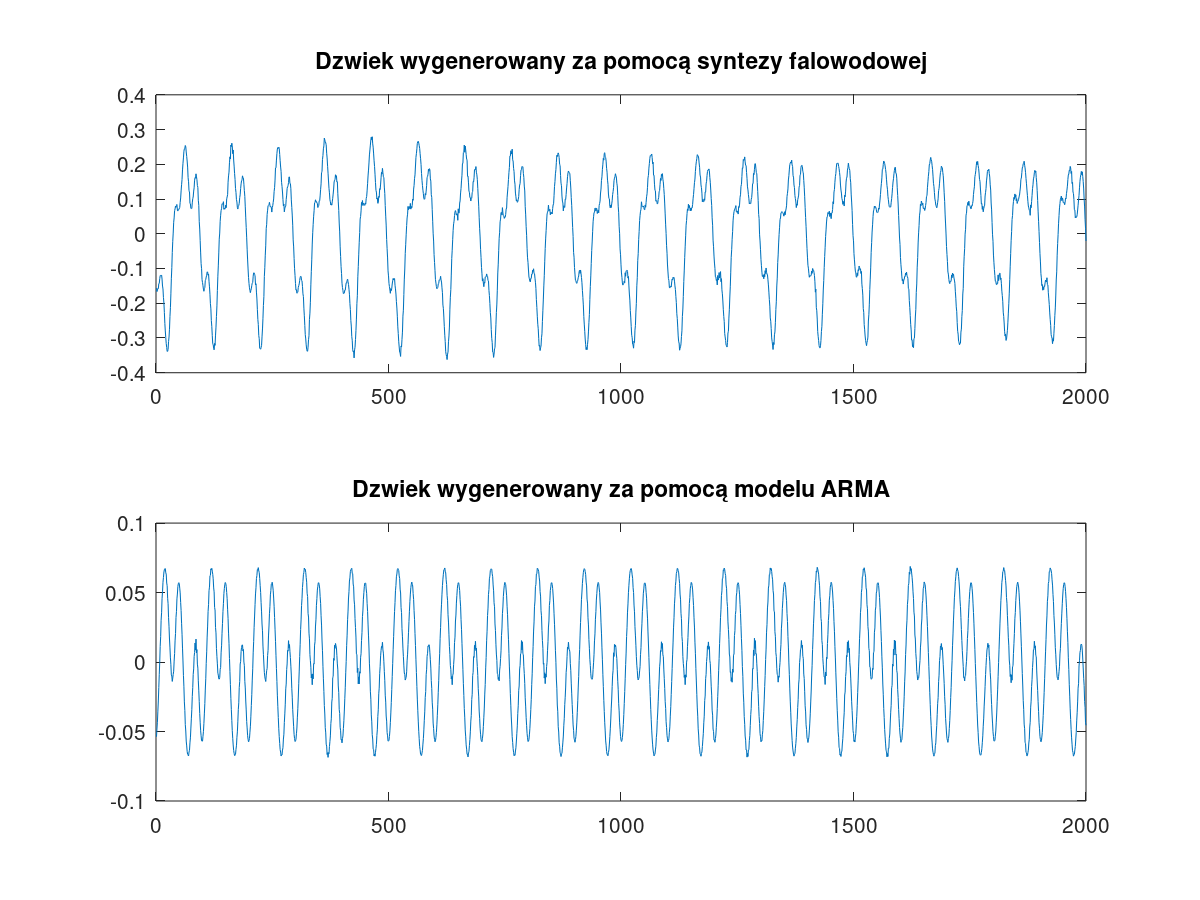
\includegraphics[width=12cm]{grafiki/flute_porownanie_syntez_symulacja}
	\captionsetup{justification=centering}
	\caption{Porównanie symulacji dzwieku fletu dla syntezy falowodowej i syntezy za pomocą modelu ARMA fletu.}
	\label{rys:por_synt_flet}
\end{figure}

Można zauważyć, iż porównanie syntezy instrumentu dętego, które zostało przedstawione na rysunku \ref{rys:por_synt_flet}, dało zupełnie różne wyniki dla obu metod. Po odpowiednim doborze parametrów modelu falowodowego, takich jak wzmocnienie sprzężenia pętli zamkniętej oraz wartość opóźnienia, uzyskane brzmienie jest bardziej zbliżone do barwy fletu. Jego barwa zmienia się w czasie. W celu otrzymania lepszych wyników syntezy za pomocą modelu ARMA, należałoby prawdopodobnie użyć modelu zmiennego w czasie (kilku modeli). Dodatkowo, aby generowany dźwięk był bardziej zbliżony do naturalnego, zidentyfikowany model powinien być wyższego rzędu.

%	\include{chapter6}
%	\chapter{Badanie układu sterowania}


Lorem ipsum dolor sit amet, consectetur adipiscing elit, sed do eiusmod tempor incididunt ut labore et dolore magna aliqua. Ut enim ad minim veniam, quis nostrud exercitation ullamco laboris nisi ut aliquip ex ea commodo consequat. Duis aute irure dolor in reprehenderit in voluptate velit esse cillum dolore eu fugiat nulla pariatur. Excepteur sint occaecat cupidatat non proident, sunt in culpa qui officia deserunt mollit anim id est laborum.


	\chapter{Podsumowanie}
% Czy udalo sie osiagnac cel pracy. Czy udalo sie spelnic te myslniki co mamy we wstepie

% Synteza subtraktywna - porownanie do normalnego instrumentu. Wypada spoko. Filtry faktycznie filtrują. Trzeba uwazac na efekt gibbsa.

% Synteza addytywna - organy Hammonda brzmia dobrze. Moznaby dorzucic jeszcze efekty dzwiekowe. Ogolnie synteza jest ograniczona przez to ze duza zlozonosc obliczeniowa. w przyszlosci moze sie uda prawdziwe nasladowac nią z szumem np

% Synteza FM -- Udalo sie zbadac algorytmy modulujace fale sinusoidalne, dzieki ktorym uzyskano ciekawe brzmienia. Udalo sie uzyskac dzwon. CD>>>> Pelka??

% Synteza matematyczna -- Porownano dwa instrumenty pod wzgledem syntezy falowodowej. Udalo sie uzyskac dzwieki w symulacji. Na procesorze jest ciezko, duza zlozonosc obliczeniowa dla skomplikowanych modeli. A skomplikowane modele potrzebne zeby brzmienie bylo mozliwe do osiagniecia instrumentow roznych. Duza precyzja -- nie dzialalo na floatach.

% TRUDNOSCI:
%	- skompilkowana architektura płyty PADK
%	- slabe wsparcie ze strony producenta - jeden z nich nie istnieje
%	- przenoszenie kodu na DSP, wymaga optymalizacji

% Czy ogolnie jakosc dzwiekow uzyskanych jest dobra
% Czy udalo sie zrobic lepszy syntezator niz rynkowy - no nie, bo to tylko prototyp.



	\listoffigures      % spis obrazków
	\listoftables

	\bibliographystyle{plain}                       % styl bibliografi
	\begin{thebibliography}{20}                      % pocz¹tek œrodowiska
		\small              % spisy i bibliografie sk³adamy mniejszym stopniem pisma
		% WSTEP
		\bibitem{historia_instr}
		Mlodytechnik.pl: \emph{https://mlodytechnik.pl/eksperymenty-i-zadania-szkolne/wynalazczosc/29983-historia-wynalazkow-instrumenty-muzyczne}, (data dostępu 09.09.2020 r.).
		
		% WPROWADZENIE
		\bibitem{dzwiek_pwn}
		Encyklopedia PWN, \emph{https://encyklopedia.pwn.pl/haslo/dzwiek}, (data dostępu 23.07.2020 r.)
		
		\bibitem{synth_brief_intro}
		Martinez-Zorrilla D.:\emph{Synthesizers: A Brief Introduction}, Universitat Oberta de Catalunya, January 2008.

		\bibitem{metody_syntezy}
		Rolonen T., Valimaki V., Karjalainen M.: \emph{Evaluation of Modern Sound Synthesis Methods}, ISSN 1239-1867, Espoo, 1998.

		\bibitem{bilbao}
		Bilbao S.: \emph{https://ccrma.stanford.edu/\textasciitilde bilbao/booktop/node12.html}, online book, (data dostępu 08.08.2020 r.).
		
		\bibitem{czyzewski_dzwiek_cyfrowy}
		Czyżewski A.:\emph{Dźwięk cyfrowy}, Akademicka Oficyna Wydawnicza EXIT, Warszawa 1998.
		 
 		\bibitem{misra_cook_przetw_syg}
		Misra A., Cook P. R.: \emph{Toward synthesized environments: A Survey Of Analysis And Synthesis Methods For Sound Designers And Composers}, Princeton University, Departament of Computer Science, 2009.
		
		\bibitem{synthtopia}
		Synthtopia: \emph{https://www.synthtopia.com/content/2019/01/11/analog-vs-digital-synthesizer-blind-test/}, (data dostępu 09.08.2020 r.).

		\bibitem{andertons}
		Blog Andertons Music CO.: \emph{https://www.synthtopia.com/content/2019/01/11/analog-vs-digital-synthesizer-blind-test/}, (data dostępu 09.08.2020 r.).
	
		\bibitem{dokumentacja_midi}
		The MIDI Manufacturers Association, \emph{The Complete MIDI 1.0 Detailed Specification}, wersja 96.1, Los Angeles, CA, 1996 r.
		
		\bibitem{dokumentacja_PADK}
		Lyrtech, \emph{Dokumentacja Professional Audio Development Kit, Technical Reference Guide}, Wrzesień 2007.
		
		\bibitem{dokumentacja_ti6727}
		Dokumentacja procesora TMS320C6727, \emph{www.ti.com}, maj 2005.
		
		\bibitem{dokumentacja_mcasp}
	    Texas Instruments, \emph{McASP Design Guide - Tips, Tricks and Practical Examples. (SPRACK0)}, Styczeń 2019 r.
		
		\bibitem{dokumentacja_dmax}
		Texas Instruments, \emph{TMS320C672x DSP Dual Data Movement Accelerator (dMAX) - Reference Guide (SPRS268E)}, maj 2005.
		
		% SUBTRACTIVE
		\bibitem{lesnicki}	% \bibitem{etykieta}
		Le\'snicki A., \emph{Technika Cyfrowego Przetwarzania Sygna\l{}\'ow }, Wydawnictwo Politechniki Gda\'nskiej, 2016.
		
		\bibitem{schafer}
		Oppenheim A. V., Schafer R. W., \emph{Cyfrowe przetwarzanie sygnałów}, 113-114, WYD. KOMUNIKACJI I ŁĄCZNOŚCI, 1979.
		
		\bibitem{alles}
		Alles H. G., \emph{Music Synthesis Using Real Time Digital Techniques}, Proc. IEEE, Vol. 68, No. 4, Apr. 1980, 439-440.

		% ADDITIVE
		\bibitem{add_defins}
		Wikipedia, The Free Encyclopedia: \emph{https://en.wikipedia.org/wiki/Additive\_synthesis\#Definitions}, (data dostępu 09.09.2020 r.).
		
		\bibitem{add_time_varying}
		Roads C. [et al.], \emph{The Computer Music Tutorial}, The MIT Press, Massachusetts Institute of Technology, 1996, Cambridge, s. 140-141.
		
		\bibitem{add_szum}
		Smith J. O., \emph{Spectral Audio Signal Processing}, \emph{https://ccrma.stanford.edu/\textasciitilde jos/sasp/S\_N\_Synthesis.html}, online book, 2011 edition, (data dostępu 09.09.2020 r.).
		
		\bibitem{add_imp_meth}
		Wikipedia, The Free Encyclopedia:
		\emph{https://en.wikipedia.org/wiki/Additive\_synthesis\#Implementation\_methods}, (data dostępu 09.09.2020 r.).
		
		\bibitem{add_ograniczenia}
		Smith J. O., \emph{Spectral Audio Signal Processing}, \emph{https://ccrma.stanford.edu/\textasciitilde jos/pasp/Additive\_Synthesis.html}, online book, 2011 edition, (data dostępu 09.09.2020 r.).
		
		\bibitem{add_wavetab_synt}
		Bristow-Johnson R., \emph{Wavetable Synthesis 101, A Fundamental Perspective}, Wave Mechanics Inc., Burnlington VT, USA, January 1996.
		
		\bibitem{add_ifft_orig}
		Rodet X., Depalle P., \emph{Synthese additive par FTT inverse}, Rapport Interne IRCAM, Paris 1990.
		
		\bibitem{add_ifft_method}
		Freed A., Rodet X., Depalle P., \emph{Synthesis and Control of Hundreds of Sinusoidal Partials on A Desktop Computer without Custom Hardware}, ICSPAT 92, San Jose, USA, 1992.
		
		\bibitem{add_hammond_soundonsound}
		Sound On Sound, \emph{https://www.soundonsound.com/techniques/synthesizing-tonewheel-organs-part-1}, (data dostępu 09.09.2020 r.).
		
		% FM
		\bibitem{chowning}
		John M. Chowning, \emph{The Synthesis of Complex Audio Spectra by Means of Frequency Modulation}, 526-534, 1973, https://web.eecs.umich.edu/\textasciitilde fessler/course/100/misc/chowning-73-tso.pdf, (data dostępu 25.08.2020 r.)
		
		\bibitem{oland}
		Anders Øland, Roger B. Dannenberg, \emph{FM Synthesis},	Carnegie Mellon University, http://www.cs.cmu.edu/\textasciitilde music/icm-online/readings/fm-synthesis/fm\_synthesis.pdf, (data dostępu 07.09.2020 r.)
		
		% VIOLIN
		\bibitem{bowed_smith}      % \bibitem{etykieta}
		Julius Orion Smith III \emph{Techniques for digital filter design and system identification with application to the violin}, June 1983.
		
		\bibitem{bowed_2}
		Mark Sterling, Mark Bocko \emph{Empirical physical modeling for bowed string instruments}
		
		\bibitem{bowed_3}
		Smith, J.O. \emph{Physical Audio Signal Processing}, https://ccrma.stanford.edu/\textasciitilde jos/pasp, książka internetowa, (data dostępu 30.05.2020r.).
		
		\bibitem{bowed_4}
		Jan Markus Holm, \emph{Modeling and modification of violin body modes for sound synthesis}
			
		\bibitem{allpass}
		Jukka Rauhala and Vesa Välimäki, \emph{Tunable Dispersion Filter Design for Piano Synthesis}, IEEE SIGNAL PROCESSING LETTERS, VOL. 13, NO. 5, MAY 2006, https://ieeexplore-1ieee-1org-1000007n7096b.han.bg.pg.edu.pl/stamp/stamp.jsp?tp=\&arnumber=1618690, data dostępu 14.09.2020 r.
		
		% FLUTE
		\bibitem{flute_klarnet}
		Sterling M., X. Dong, M. Bocko, \emph{Representation of solo clarinet music by physical modeling synthesis}, University of Rochester, Rochester NY, USA, March 2008.
		
		\bibitem{flute_flecista}
		Montgermont N., Fabre B., Cuadra P., \emph{Gesture synthesis: basic control of a flute physical model}, The Journal of the Acoustical Society of America, June 2008.
		
		\bibitem{flute_cook}
		Cook P. R., \emph{A meta-wind-instrument physical model, and a meta-controller for real time performance control}, Stanford CCRMA, Stanford, CA, USA, 1992.
		
		\bibitem{flute_prezka}
		Hemingway B., G. Charles, \emph{Lectures: 15 - Waveguide instruments}, University of Washington, Seattle, USA.
	\end{thebibliography}
	
\end{document}